\documentclass[10pt,journal,final,letterpaper]{./../Styles/IEEEtran}

\usepackage{amsmath,amssymb}
\usepackage{acronym,etoolbox}
\usepackage{graphicx,epstopdf}
\usepackage[ruled]{algorithm2e}
\usepackage[usenames,dvipsnames]{xcolor}
\usepackage[subrefformat=parens,labelformat=parens,labelseparator=period,caption=false,font=footnotesize]{subfig}
\usepackage{multirow,cite,setspace,fixltx2e,lineno,verbatim,mathtools,url,cases}

\graphicspath{{./../Figures/}{./../Figures/Linux/}{./../Figures/Review/}}
\DeclareGraphicsExtensions{.eps}

\setlength{\floatsep}{0.75\baselineskip}
\setlength{\textfloatsep}{0.75\baselineskip}

\ifCLASSINFOpdf
\epstopdfsetup{update,prepend,prefersuffix=false,suffix=}
\DeclareGraphicsRule{.eps}{pdf}{.pdf}{`epstopdf #1}
\pdfcompresslevel=9
\fi 

\newcommand{\mbf}[1]{\mathbf{#1}}
\newcommand{\me}[1]{\( #1 \)}
\newcommand{\mc}[1]{\mathcal{#1}}
\newcommand{\fall}{\forall}
\newcommand{\set}[1]{\left \lbrace #1 \right \rbrace }
\newcommand{\mvec}[2]{\mathbf{#1}_{#2}}
\newcommand{\ith}[1]{{#1}^\mathrm{th}}
\newcommand{\pr}[1]{{#1}^\prime}
\newcommand{\mbfa}[1]{{\boldsymbol{#1}}}
\newcommand{\herm}{\mathrm{H}}
\newcommand{\sset}[1]{\left [ #1 \right ]}
\newcommand{\rfrac}[2]{{}^{#1}/{}_{#2}}
\newcommand{\eqspace}{\IEEEeqnarraynumspace}
\newcommand{\enoise}{\widetilde{N}_0}
\newcommand{\eqsub}{\IEEEyessubnumber}
\newcommand{\eqsubn}{\IEEEyesnumber \IEEEyessubnumber*}
\newcommand{\neqsub}{\IEEEnosubnumber}
\newcommand{\review}[1]{{\textcolor[rgb]{0 0 0.6}{#1}}}
\newcommand{\trace}{\mathrm{tr}}
\newcommand{\tran}{\mathrm{T}}
\newcommand{\R}[1]{\label{#1}\linelabel{#1}}
\newcommand{\lr}[1]{page~\pageref{#1}, line~\lineref{#1}}
\newcommand{\eqn}[1]{\(#1\)}
\newcommand{\mx}{\mbf{m}}
\newcommand{\my}{\mbf{w}}
\newcommand{\mz}{\mbfa{\gamma}}
\newcommand{\mxb}{{{\mbf{m}}}}
\newcommand{\myb}{{{\mbf{w}}}}
\newcommand{\iterate}[2]{{#1}^{(#2)}}
\newcommand{\iter}[3]{{#1}_{#2}^{(#3)}}
\newcommand{\ma}{\mbf{x}}
\acrodef{MSE}{mean squared error}
\acrodef{IBC}{interference broadcast channel}
\acrodef{MC}{multi-cell}
\acrodef{BS}{base station}
\acrodef{MIMO}{multiple-input multiple-output}
\acrodef{SISO}{single-input single-output}
\acrodef{MU}{multiple-users}
\acrodef{OFDM}{orthogonal frequency division multiplexing}
\acrodef{WSRM}{weighted sum rate maximization}
\acrodef{QoS}{quality of service}
\acrodef{SCA}{successive convex approximation}
\acrodef{SNR}{signal-to-noise ratio}
\acrodef{MMSE}{minimum \acl{MSE}}
\acrodef{SIR}{signal-to-interference ratio}
\acrodef{SINR}{signal-to-interference-plus-noise ratio}
\acrodef{Q-WSRM}{queue \acl{WSRM}}
\acrodef{QM}{queue minimizing}
\acrodef{SRA}{spatial resource allocation}
\acrodef{JSFRA}{joint space-frequency resource allocation}
\acrodef{WMMSE}{weighted \acl{MMSE}}
\acrodef{KKT}{Karush-Kuhn-Tucker}
\acrodef{GP}{geometric programming}
\acrodef{SOC}{second-order cone}
\acrodef{BCDM}{block coordinate descent method}
\acrodef{ADMM}{alternating directions method of multipliers}
\acrodef{PD}{primal decomposition}
\acrodef{DD}{dual decomposition}
\acrodef{FFR}{fractional frequency reuse}
\acrodef{DC}{difference of convex}
\acrodef{Q-WSRME}{\ac{Q-WSRM} extended}

\newtoggle{includereview}
\newtoggle{enable_dist_fig}
\newtoggle{single_column}
\togglefalse{single_column}
\togglefalse{enable_dist_fig}

\iftoggle{single_column}{
	\doublespacing
}

\title{Traffic Aware Resource Allocation Schemes for Multi-Cell \acs{MIMO}-\acs{OFDM} Systems}
\author{
	\IEEEauthorblockN{Ganesh Venkatraman \IEEEmembership{Student Member,~IEEE}\thanks{This work has been supported by the Finnish Funding Agency for Innovation (Tekes), Nokia Networks, Xilinx, Elektrobit and the Academy of Finland. Part of this work is presented in ICASSP 2014.}, Antti T\"{o}lli \IEEEmembership{Senior Member,~IEEE}, Markku Juntti \IEEEmembership{Senior Member,~IEEE}, and Le-Nam Tran \IEEEmembership{Member,~IEEE}}\thanks{
	G. Venkatraman, A. T\"{o}lli and M. Juntti are with Centre for Wireless Communications (CWC), Department of Communications Engineering (DCE), University of Oulu, Oulu, FI-90014, (e-mail: \{ganesh.venkatraman, antti.tolli, markku.juntti\}@ee.oulu.fi)}\thanks{L.-N. Tran was with Centre for Wireless Communications (CWC), Oulu, FI-90014. He is now with the Department of Electronic Engineering, Maynooth University, Maynooth, Co. Kildare, Ireland, (e-mail:ltran@eeng.nuim.ie)}}

\begin{document}

\maketitle

\begin{abstract}
%We consider a downlink multi-cell \ac{MIMO} \ac{IBC} using \ac{OFDM} with \acl{MU} contending for space-frequency resources in a given scheduling instant. The problem is to determine the transmit precoders by the \acp{BS} in a coordinated approach to minimize the total number of backlogged packets in the \acp{BS}. The \ac{Q-WSRM} is a conventional design objective with the number of backlogged packets reflected in the corresponding weights, \textit{i.e}, the longer the queue size, the higher the priority. In contrast, we design the precoders jointly across the space-frequency resources by minimizing the total user queue deviations. The problem is nonconvex, and, therefore, we employ \ac{SCA} to solve the problem by a sequence of convex subproblems using the first order Taylor approximation. At first, we propose a centralized \ac{JSFRA} solution using two different formulations by employing the \ac{SCA} technique, namely the sum rate formulation and the \ac{MSE} reformulation. We then introduce distributed precoder designs using primal and \ac{ADMM} for the \ac{JSFRA} solutions. Finally, we propose a practical distributed iterative precoder design based on the \ac{MSE} reformulation approach by solving the \acl{KKT} conditions with closed form expressions. Numerical results are used to compare the proposed algorithms to the existing solutions.
%
%we address the queue minimizing downlink precoder design as a joint nonconvex optimization problem over space-frequency resources. We employ \ac{SCA} technique to solve the problem by a sequence of convex subproblems using inner approximations. Initially, we discuss the centralized \acl{JSFRA} solutions based on \ac{SCA} as well as by \acl{MSE} reformulation. Then we extend the distributed precoder design for the centralized schemes using primal and \ac{ADMM} method. Finally, we discuss the distributed precoder design problem by solving the \ac{KKT} expressions to obtain the closed form solutions for the transmit and the receive precoders. Numerical results are shown to compare them.
%
%We consider a downlink multi-cell \ac{MIMO} \ac{IBC} using \ac{OFDM} with \acl{MU} contending for space-frequency resources in a given scheduling instant. The problem is to design transmit precoders efficiently to minimize the total number of backlogged packets waiting at the coordinating \acp{BS}. Conventionally, the \ac{Q-WSRM} formulation with the number of backlogged packets as the corresponding weights is used to design the precoders. However, in the proposed \ac{JSFRA} scheme, the precoders are designed jointly across the space-frequency resources for all users by minimizing the total number of backlogged packets in each transmission instant, thereby performing user scheduling implicitly. Since the problem is nonconvex, we solve the \ac{JSFRA} formulation iteratively by solving an approximate convex subproblem in each iteration by updating the operating point. The \ac{JSFRA} formulation is solved using two different techniques, namely by the \ac{SINR} relaxation method and by the \ac{MSE} reformulation approach. We then discuss the distributed precoder designs using primal decomposition and the \ac{ADMM} for the proposed \ac{JSFRA} solutions. Finally, we propose a practical iterative precoder design by solving the \acl{KKT} expressions for the \ac{MSE} reformulation that requires minimal information exchange for each update. Numerical results are used to compare the proposed algorithms to the existing solutions.
We consider a downlink multi-cell \ac{MIMO} \ac{IBC} using \ac{OFDM} with \acl{MU} contending for space-frequency resources in a given scheduling instant. The problem is to design precoders efficiently to minimize the number of backlogged packets queuing in the coordinating \acp{BS}. Conventionally, the \ac{Q-WSRM} formulation with the number of backlogged packets as the corresponding weights is used to design the precoders. In contrast, we propose \ac{JSFRA} formulation, in which the precoders are designed jointly across the space-frequency resources for all users by minimizing the total number of backlogged packets in each transmission instant, thereby performing user scheduling implicitly. Since the problem is nonconvex, we use the combination of \ac{SCA} and \ac{AO} to handle nonconvex constraints in the \ac{JSFRA} formulation. In the first method, we approximate the \ac{SINR} by convex relaxations, while in the second approach, the equivalence between the \ac{SINR} and the \ac{MSE} is exploited. We then discuss the distributed approaches for the centralized algorithms using primal decomposition and \ac{ADMM}. Finally, we propose a practical iterative precoder design by solving the \acl{KKT} expressions for the \ac{MSE} reformulation that requires minimal information exchange for each update. Numerical results are used to compare the proposed algorithms to the existing solutions.
%We consider a downlink multi-cell \ac{MIMO} \ac{IBC} using \ac{OFDM} with \acl{MU} contending for space-frequency resources in a given scheduling instant. The problem is to design transmit precoders efficiently to minimize the total number of backlogged packets queuing at the coordinating \acp{BS}. Conventionally, the \ac{Q-WSRM} formulation with the number of backlogged packets as the corresponding weights is used to design the precoders. Alternatively, we propose the \ac{JSFRA} scheme, which design the precoders jointly across the space-frequency resources for all users to minimize the number of backlogged packets in each transmission instant, thereby performing scheduling implicitly. Since the \ac{JSFRA} problem is nonconvex, we first propose two centralized iterative algorithms based on the combination of \ac{SCA} and the \ac{AO}. The proposed algorithms solve a sequence of convex problems obtained by fixing a subset of otpimization variables or by approximating the nonconvex constraints by the convex ones. In the first method we directly aprroximate the signal-to-interferenceplus-noise ratio (SINR) by convex formulations, while in the second one the equivalcen between rate function and mean squre error is exploited. Based on the centralized algorithms we then discuss the distributed precoder designs using primal decomposition and the alternating directions method of multipliers (ADMM). Finally, we also propose a more practical iterative precoder design by directly solving the Karush-Kuhn-Tucker system of equations for the MSE reformulation that is numerically shown to require minimal information exchange for each update. Numerical results are provided to demonstrate the superior performance of the proposed methods over the existing solutions.


%Since the problem is nonconvex, we solve the \ac{JSFRA} formulation iteratively by solving an approximate convex subproblem in each iteration by updating the operating point. The \ac{JSFRA} formulation is solved using two different techniques, namely by the \ac{SINR} relaxation method and by the \ac{MSE} reformulation approach. We then discuss the distributed precoder designs using primal decomposition and the \ac{ADMM} for the proposed \ac{JSFRA} solutions. Finally, we propose a practical iterative precoder design by solving the \acl{KKT} expressions for the \ac{MSE} reformulation that requires minimal information exchange for each update. Numerical results are used to compare the proposed algorithms to the existing solutions.


%Since the considered JSFRA  problem is nonconvex, we first propose two centralized iterative algorithms based on a combination of successive convex approximation and alternating optimization. The proposed algorithms solve a sequence of convex problems obtained by fixing a subset of otpimization variables or by approximating the nonconvex constraints by the convex ones. In the first method we directly aprroximate the signal-to-interferenceplus-noise ratio (SINR) by convex formulations, while in the second one the equivalcen between rate function and mean squre error is exploited. Based on the centralized algorithms we then discuss the distributed precoder designs using primal decomposition and the alternating directions method of multipliers (ADMM). Finally, we also propose a more practical iterative precoder design by directly solving the Karush-Kuhn-Tucker system of equations for the MSE reformulation that is numerically shown to require minimal information exchange for each update. Numerical results are provided to demonstrate the superior performance of the proposed methods over the existing solutions.
\end{abstract}

\begin{IEEEkeywords}
Convex approximations, \ac{MIMO}-\acs{IBC}, \ac{MIMO}-\ac{OFDM}, precoder design, \acs{SCA}, \acs{WSRM}.
\end{IEEEkeywords}

\acresetall 
\acused{MU}

\section{Introduction} \label{sec-1}

The last mile wireless connectivity poses significant bottleneck in the overall data traffic for the interconnected networks. The main challenges in the wireless networks are due to the scarcity of the available resources either in terms of power or spectrum usage and the complexity of the receiver algorithms which impacts the mobile battery consumption. In order to overcome the receiver complexity, \ac{OFDM} is introduced for the wide band transmissions. To improve data rate, multiple antennas are installed at \acp{BS} and/or at user terminals to avail additional freedom in the form of spatial dimension. The inclusion of \ac{MIMO} technique in wireless networks provides higher data rate or lower outage for the same transmission power and bandwidth.

In a network with multiple \acp{BS} serving multiple users (\acs{MU}), the main driving factor for the transmission are the packets waiting at each \ac{BS} corresponding to the different users present in the network. These available packets are transmitted over the shared wireless resources subject to certain system limitations and constraints. We consider the problem of transmit design over the space-frequency resources provided by the \acs{MIMO}-\ac{OFDM} framework in the downlink broadcast transmission to minimize the number of queued packets. Since the space-frequency resources are shared by multiple users associated with different \acp{BS}, the problem of interest can be viewed as a resource allocation to minimize the total number of backlogged packets of all \acp{BS}.

In general, the resource allocation problems are solved by assigning a binary variable to each user indicating the presence or the absence on a particular resource. In contrast to that, we use the transmit beamformers, which are the complex vectors, as a decision variable in determining the presence or the absence of a user on a particular resource. The purpose of using the transmit beamformers for the scheduling is two fold. Firstly, it determines the transmission rate on a certain resource and secondly, by making the transmit beamformer to be a zero vector, the corresponding user will not be scheduled on a certain resource.

In order to reduce the complexity involved in the precoder design problem, linear precoding are assumed at the \acp{BS} and detection is used at users. The queue minimizing network optimization objective is used to design the beamformers across the coordinating \acp{BS}, since the transmissions are guided by the available backlogged packets. To achieve the best performance, we propose a joint resource allocation scheme over the space and frequency dimensions among the coordinating \acp{BS} to minimize the time that the packets stay in the queues prior to the transmission, and, hence, to avoid packet drops as an indirect objective.

The queue minimizing precoder designs are closely related to the \ac{WSRM} problem with additional rate constraints determined by the number of backlogged packets for each user in the system. The topics on \ac{MIMO} \ac{IBC} precoder design have been studied extensively with different performance criteria in the literature. Due to the nonconvex nature of the \ac{MIMO} \ac{IBC} precoder design problems, the \ac{SCA} method has become a powerful tool to deal with these problems. For example, in \cite{sin_algorithm}, the nonconvex part of the objective is linearized around an operating point in order to solve the \ac{WSRM} problem in an iterative manner. Similar approach of solving the \ac{WSRM} problem via arithmetic-geometric inequality is proposed in \cite{tran2012fast}.

The connection between the achievable capacity and the \ac{MSE} for the received symbol by using the fixed \ac{MMSE} receivers as shown in \cite{viswanath1999optimal,mse_duality} can also be used to solve the \ac{WSRM} problem. In \cite{christensen2008weighted,wmmse_shi}, the \ac{WSRM} problem is reformulated via \ac{MSE}, casting the problem as a convex one for fixed linearization coefficients. In this way, the original problem is expressed in terms of the \ac{MSE} weight, precoders, and decoders. Then the problem is solved using an alternating optimization method, i.e., finding a set of variables while the remaining others are fixed. The \ac{MSE} reformulation for the \ac{WSRM} problem is also studied in \cite{hong2012decomposition} by using the \ac{SCA} to solve the problem in an iterative manner. Additional rate constraints based on the \ac{QoS} requirements are included in the \ac{WSRM} problem and solved via \ac{MSE} reformulation in \cite{kaleva2013primal,kaleva2013decentralized}.

The problem of precoder design for the \ac{MIMO} \ac{IBC} system are solved either by using a centralized controller or by using decentralized algorithms where all \acp{BS} handles their own subproblems and exchange limited information via backhaul. The distributed approaches are based on primal, dual or \ac{ADMM} decomposition, which are discussed in a detailed manner in \cite{palomar2006tutorial,boyd2011distributed}. In the  primal decomposition, the so-called coupling interference variables are fixed for the subproblem at each \ac{BS} to find the optimal precoders. The fixed interference are then updated by using the subgradient method as discussed in \cite{pennanen2011decentralized}. The dual and \ac{ADMM} approach controls the distributed subproblems by fixing the \emph{`interference price'} for each \ac{BS} as detailed in \cite{tolli2011decentralized}.

By adjusting the weights in the \ac{WSRM} objective properly, we can find arbitrary rate-tuple in the rate region that maximizes the suitable objective measures. For example, if the weight of each user is set to be inversely proportional to his/her average data rate, the corresponding problem guarantees fairness on an average among the users. As an approximate method, we may assign weights based on the current queue size of users. More specifically, the queue states can be incorporated to traditional weighted sum rate objective $\sum_k w_k R_k$ by replacing the weight $w_k$ with the corresponding queue state $Q_k$ or a function of it,  which is the outcome of minimizing the Lyapunov drift between the current and the future queue states \cite{tassiulas,neely2010stochastic}. In backpressure algorithm, the differential queues between the source and the destination nodes are used as the weights scaling the transmission rate \cite{georgiadis2006resource}.

Earlier studies on the queue minimization problem was summarized in the survey paper \cite{berry2004cross}. In particular, the problem of power allocation to minimize the number of backlogged packets was considered in \cite{qps_cioffi} using geometric programming. Since the problem addressed in \cite{qps_cioffi} assumed single antenna transmitters and receivers, the queue minimizing problem reduces to the optimal power allocation problem. In the context of wireless networks, the backpressure algorithm mentioned above was extended in \cite{weeraddana2011resource} by formulating the corresponding user queues as the weights in the \ac{WSRM} problem.

In this paper, we consider the problem of precoder design across the space-frequency resources to minimize the total number of queued packets of all \acp{BS}. For this highly nonconvex problem, we first propose two centralized methods. In the first method, we relax the nonconvex constraint by the first order Taylor approximation around an operating point, which is updated in an iterative manner until convergence or to a certain accuracy. In the second method, we reformulate the \ac{JSFRA} problem using the \ac{MSE} equivalence with the rate expression to solve for the optimal precoders. For distributed implementation, we further proposed decentralized approaches based on primal and \ac{ADMM} scheme to identify the precoders independently across the \acp{BS} by exchanging limited information via back-haul. We also proposed an iterative algorithm by solving the \ac{KKT} equations, which can be implemented easily in a distributed manner.

The remainder of this paper is organized as follows. In Section \ref{sec-2-3.2}, we introduce the system model and the problem formulation for the queue minimizing precoder design. Existing and the proposed precoder designs for the \ac{JSFRA} problem are presented in Section \ref{sec-3}. The distributed solutions are provided in Section \ref{sec-4} followed by the simulation results in Section \ref{sec-5}. Conclusions are drawn in Section \ref{sec-6}.

\section{System Model and Problem Formulation} \label{sec-2-3.2}
\subsection{System Model} \label{sec-2}
We consider a downlink \ac{MIMO} \ac{BC} scenario in an \ac{OFDM} framework with \me{N} sub-channels and \me{N_B} \acp{BS} each equipped with \me{N_T} transmit antennas, serving \me{K} users each with \me{N_R} receive antennas. The set of users associated with \ac{BS} \me{b} is denoted by \me{\mathcal{U}_b} and the set \me{\mathcal{U}} represents all users in the system, i.e., \me{\mathcal{U} =\underset{b\in \mathcal{B}}{\cup }\mathcal{U}_b}, where the set \me{\mathcal{B}} holds the coordinating \acp{BS}. The serving \ac{BS} of user \me{k} is denoted by \me{b_k\in \mathcal{B}}. We denote by \me{\mathcal{C} = \set{1,2,\dotsc,N}} the set of all sub-channel indices available in the system.

In this paper we adopt linear beamforming technique at \acp{BS}. Specifically, the data symbols \me{d_{l,k,n}} for  user \me{k} on the \me{l^\mathrm{th}} spatial stream over the sub-channel \me{n} is multiplied with the beamformer \me{\mvec{m}{l,k,n} \in \mathbb{C}^{N_T \times 1}} for transmission.   In order to detect  multiple spatial streams at the receiver, a receive beamforming vector \me{\mvec{w}{l,k,n}} is employed at each user. Consequently, the received data symbol corresponding to the \me{l^\mathrm{th}} spatial stream over sub-channel \me{n^\mathrm{th}} at user $k$ is given by
\begin{equation}\label{eqn-1}
\hat{d}_{l,k,n} = \mvec{w}{l,k,n}^\herm \mvec{H}{b_k,k,n} \,\mvec{m}{l,k,n} d_{l,k,n} + \mvec{w}{l,k,n}^\herm \sum_{i \in \mc{U} \backslash \set{k}} \mvec{H}{b_i,k,n} \sum_{j = 1}^L \mvec{m}{j,i,n}d_{j,i,n} + \mvec{w}{l,k,n}^\herm \mvec{n}{k,n}
\end{equation}
where \me{\mvec{H}{b,k,n} \in \mathbb{C}^{N_R \times N_T}} with rank \me{L = \min(N_R,N_T)} is the channel between the \ac{BS} \me{b} and  user \me{k} on the sub-channel \me{n}, and \me{\mvec{n}{k,n}} \me{\sim \mc{CN}(0,N_0)} is the additive noise vector for the user \me{k} on the \me{n^\mathrm{th}} sub-channel and \me{l^\mathrm{th}} spatial stream. Assuming  \me{||\mvec{w}{l,k,n}||_{2}^{2} = 1} and independent detection of data streams, we can write the signal-to-interference-plus-noise ratio (SINR) as
\begin{equation}\label{eq:SINR}
\gamma_{l,k,n} = \dfrac{\left |\mvec{w}{l,k,n}^\herm \, \mvec{H}{b_k,k,n} \, \mvec{m}{l,k,n} \right |^2}{N_0 + \sum_{(j,i) \neq (l,k)} |\mvec{w}{l,k,n}^\herm \mvec{H}{b_i,k,n} \mvec{m}{j,i,n} |^2}.
\end{equation}
With the infinite buffer model assumption, let \me{Q_k} be the number of backlogged packets which are destined for the user \me{k} at a given scheduling instant. The queue dynamics of the user \me{k} are modeled using the Poisson arrival process with the average packet arrivals of \me{A_k = \mathbf{E}_i\{\lambda_k\}} packets/bits, where \me{\lambda_k(i) \sim \mathrm{Pois}(A_k)} represents the instantaneous number of packets or bits arriving for the user \me{k} at the \me{{i}^\mathrm{th}} instant. The total number of queued packets at the \me{{(i+1)}^\mathrm{th}} instant for the user \me{k}, represented by \me{Q_k(i+1)}, follows
\begin{equation}
Q_k(i+1) = \Big [ Q_k(i) - t_k(i) \Big ]^+ + \lambda_k(i),
\label{eqn-2a}
\end{equation}
where \me{[x]^+ \equiv \max{ \lbrace x,0  \rbrace}} and \me{t_k} denotes the transmission in bits for user \me{k}. For a \ac{MIMO} \ac{OFDM} system,
\begin{equation}
t_k(i) = \sum_{n = 1}^N \, \sum_{l = 1}^L \, t_{l,k,n}(i),
\end{equation}
where \me{t_{l,k,n}} denotes the transmitted bits over \me{\ith{l}} spatial stream on the \me{\ith{n}} sub-channel. The maximum rate achieved over the \me{(l,n)} space-frequency resource is given by \me{\log_2(1 + \gamma_{l,k,n})}\footnote{assuming Gaussian signaling} for a given \ac{SINR} of \me{\gamma_{l,k,n}}. Note that the units of \me{t_k} and \me{Q_k} are in bits defined per channel use.
\subsection{Problem Formulation} \label{sec-3.2}
To minimize the total number of backlogged packets, we consider minimizing the weighted \me{\ell_{q}}-norm of the queue deviation given by
\begin{equation}
v_k =  Q_k - t_k = Q_k - \sum_{n = 1}^N \sum_{l = 1}^{L} \log_2(1+\gamma_{l,k,n}).
\label{eqn-4.2}
\end{equation}

Explicitly, the objective of the problem considered is given by \me{\sum_{k \in \mc{U}} \, a_k | v_k |^q}. With this objective function, the weighted queued packet minimization formulation is given by
\begin{IEEEeqnarray}{rCl}\label{eqn-3}
\underset{\substack{\mvec{M}{k,n},\mvec{W}{k,n}}}{\text{minimize}} &\quad& \|  \tilde{\mbf{v}}  \|_q\IEEEyessubnumber \\
\text{subject to} & \quad&\sum_{n = 1}^N \sum_{k \in \mathcal{U}_b} \text{tr} \, (\mvec{M}{k,n} \mvec{M}{k,n}^\herm) \leq P_{{\max}}, \fall b, \IEEEyessubnumber \label{eqn-4.3}
\end{IEEEeqnarray}
where \me{\tilde{v}_k \triangleq a_k^{1/{q}}v_k} is the element of vector \me{\tilde{\mbf{v}}}, and \me{a_k} is the weighting factor which is incorporated to control user priority based on their respective \ac{QoS}, \me{\mbf{M}_{k,n} \triangleq [ \, \mvec{m}{1,k,n} \, \mvec{m}{2,k,n} \dotsc \mvec{m}{L,k,n} \,]} comprises the beamformers associated with user \me{k} for \me{n^\mathrm{th}} sub-channel transmission, and \me{\mbf{W}_{k,n} \triangleq [ \, \mvec{w}{1,k,n} \, \mvec{w}{2,k,n} \dotsc \mvec{w}{L,k,n} \,]} stacks the receive beamformers respectively\footnote{It can be easily extended for user specific streams \me{L_{k,n}} instead of using the common \me{L} streams for all users}. In \eqref{eqn-4.3}, we consider a \ac{BS} specific sum power constraint for each \ac{BS} across all sub-channels.

For practical reasons, we may impose a constraint that the maximum number of transmitted bits for the user \me{k} is limited by the total number of backlogged packets available at the transmitter. As a result, the number of backlogged packets \me{v_k} for user \me{k} remaining in the system is given by
\begin{equation} \label{rate_constraint_a}
v_k =  Q_k - \sum_{n = 1}^N \sum_{l = 1}^{L} \log_2(1+\gamma_{l,k,n}) \geq 0.
\end{equation}
The above positivity constraint need to be satisfied by \me{v_k} to avoid the excessive allocation of the resources.

Before proceeding further, we show that the constraint in \eqref{rate_constraint_a} is handled implicitly by the definition of norm \me{\ell_q} in the objective of \eqref{eqn-3}. Suppose that \me{t_k>Q_k} for certain \me{k} at the optimum, i.e., \me{-{v}_k=t_k-Q_k>0}. Then there exists \me{\delta_k>0} such that \me{-{v}^{\prime}_k=t^{\prime}_k-Q_k<-{v}_k} where \me{t^{\prime}_k=t_k-\delta_k}. Since \me{\|\tilde{\mbf{v}}\|_q=\| |\tilde{\mbf{v}}| \|_q=\||-\tilde{\mbf{v}}|\|_q}, this means that the newly created vector \me{\mbf{t}^{\prime}} achieves a smaller objective which contradicts with the fact that the optimal solution has been obtained. The choice of the norm \me{\ell_q} used in the objective function \cite{berry2004cross,qps_cioffi} alters the priorities for the queue deviation function as follows
\begin{itemize}
\item \me{\ell_{1}} results in greedy allocation \textit{i.e}, emptying the queue of users with good channel conditions before considering the users with worse channel conditions. As a special case, it is easy to see that \eqref{eqn-3} reduces to the \ac{WSRM} problem when the queue size is large enough for all users.
\item \me{\ell_{2}} prioritizes users with higher number of queued packets before considering the users with a smaller number of backlogged packets. For example, it could be more ideal for the delay limited scenario when the packet arrival rates of the users are similar, since the number of backlogged packets is proportional to the delay in the transmission following the Little's law \cite{neely2010stochastic}.
\item \(\ell_{\infty} \) minimizes the maximum number of queued packets among users with the current transmission, thereby providing queue fairness by allocating the resources proportional to the number of backlogged packets.
\end{itemize} 

\section{Proposed Queue Minimizing Precoder Designs} \label{sec-3}

% To begin with, we discuss the existing solution and its extension to solve the problem of resource allocation over multiple sub-channels. Then, we provide two approaches to solve the \ac{JSFRA} precoder design problem to minimize the total number of backlogged packets. At the end, we discuss a low complex solution for the \ac{JSFRA} problem by limiting the precoder design over each sub-channel at a given instant.

In general, the precoder design for the \ac{MIMO} \ac{OFDM} problem is highly difficult due to the combinatorial and the nonconvex nature of the problem. In addition to that, the objective of minimizing the number of the queued packets over the spatial and the sub-channel dimensions adds further complexity to the existing problem. Since the scheduling of users in each sub-channel can be made by allocating zero transmit power over certain sub-channels, the solutions provided in the paper performs both precoder design and the scheduling of users in a joint manner.

\subsection{Queue Weighted Sum Rate Maximization (\acs{Q-WSRM})} \label{sec-3.1} %\acused{Q-WSRM}
The queue minimizing algorithms have been studied extensively in the networking context to provide congestion-free routing between any two nodes in the network. One such is the \emph{backpressure algorithm} \cite{georgiadis2006resource,neely2010stochastic}. It finds an optimal control policy in the form of rate or resource allocation by considering differential backlogged packets between any two entities. %Even though the algorithm is primarily designed for the wired infrastructure, it can be extended to the wireless networks by designing the user rate variable \me{t_k} in accordance to the wireless network.

The \ac{Q-WSRM} formulation extends the \emph{backpressure algorithm} to the downlink \ac{MIMO}-\ac{OFDM} framework, in which the \acp{BS} act as the source nodes and the users as the receivers. The control policy in the form of transmit precoders aims at minimizing the number of queued packets waiting in the \acp{BS}. To find an optimal strategy, we resort to the Lyapunov theory, which is predominantly used in control theory to achieve system stability. Since at each time slot, the system is described by the channel conditions and the number of backlogged packets for each user, the Lyapunov function is used to provide a scalar measure, which grows large when the system moves towards an undesirable state \cite{neely2010stochastic}. The scalar measure for queue stability is given by
\begin{equation}
\mathrm{L}\sset{\mbf{Q}(i)} = \frac{1}{2} \, \sum_{k \in \mc{U}} Q_k^2(i)
\end{equation}
where \me{\mbf{Q}(i) = \sset{Q_1(i),Q_2(i),\dotsc,Q_K(i)}^\mathrm{T}}. It provides a scalar measure of congestion in the system \cite[Ch. 3]{neely2010stochastic}. 

To minimize the total number of backlogged packets for time instant \me{i}, the optimal transmission rate of all users is obtained by minimizing the Lyapunov drift expressed as  
\iftoggle{single_column}{
\begin{equation} \label{eqn-3.1}
\mathrm{L}\sset{\mbf{Q}(i+1)} - \mathrm{L}\sset{\mbf{Q}(i)} = \frac{1}{2} \Big [ \sum_{k \in \mc{U}} \, \Big ( \left [ Q_k(i) - t_k(i) \right ]^+ + \lambda_k(i) \Big )^2 - Q^2_k(i) \Big ].
\end{equation}}{
\begin{multline} \label{eqn-3.1}
\mathrm{L}\sset{\mbf{Q}(i+1)} - \mathrm{L}\sset{\mbf{Q}(i)} = \\ \frac{1}{2} \Big [ \sum_{k \in \mc{U}} \, \Big ( \left [ Q_k(i) - t_k(i) \right ]^+ + \lambda_k(i) \Big )^2 - Q^2_k(i) \Big ].
\end{multline}}
To eliminate the nonlinear operator \me{[x]^+}, we bound \eqref{eqn-3.1} as
\begin{equation}
\leq \sum_{k \in \mc{U}} \, \frac{\lambda^2_k(i) + t_k^2(i)}{2} + \sum_{k \in \mc{U}} Q_k(i) \set{ \lambda_k(i) - t_k(i) }
\label{drift-exp}
\end{equation}
by using the following inequality 
\begin{equation}
\sset{\max(Q-t,0) + \lambda}^2 \leq Q^2 + t^2 + \lambda^2 + 2 Q (\lambda - t).
\end{equation}
The total number of backlogged packets at any given instant \me{i} is reduced by minimizing the conditional expectation of the Lyapunov drift expression \eqref{drift-exp} given the current number of queued packets \me{\mbfa{Q}(i)} waiting in the system. The expectation is taken over all possible arrival and transmission rates of the users to obtain the optimal rate allocation strategy. 

Now, the conditional Lyapunov drift, denoted by \me{\Delta{(\mbfa{Q}(i))}}, is given by the infimum over the transmission rate as
\iftoggle{single_column}{
\begin{IEEEeqnarray}{rCl} \label{backpressure-approx} \neqsub
	\underset{\mbf{t}}{\text{inf}} &\quad& \Delta(\mbf{Q}(i)) \triangleq \mathbb{E}_{\mbfa{\lambda},\mbf{t}} \set{\mathrm{L}\sset{\mbf{Q}(i+1)} - \mathrm{L}\sset{\mbf{Q}(i)} \vert \mbf{Q}(i)} \IEEEyessubnumber \\
	&\leq& \underbrace{\mathbb{E}_{\mbfa{\lambda},\mbf{t}} \set {\sum_{k \in \mc{U}} \, \frac{\lambda^2_k(i) + t_k^2(i)}{2} \vert \mbf{Q}(i)}}_{\le B} + \sum_{k \in \mc{U}} Q_k(i) A_k(i) - \mathbb{E}_{\mbfa{\lambda},\mbf{t}}\set{\sum_{k \in \mc{U}} Q_k(i) t_k(i)  \vert \mbf{Q}(i)}, \eqsub \label{backpressure-approx-1b}
\end{IEEEeqnarray}}{
\begin{IEEEeqnarray}{CL} \label{backpressure-approx} \neqsub
	\underset{\mbf{t}}{\text{inf}} \quad & \mathbb{E}_{\mbfa{\lambda},\mbf{t}} \set{\mathrm{L}\sset{\mbf{Q}(i+1)} - \mathrm{L}\sset{\mbf{Q}(i)} \vert \mbf{Q}(i)} \eqsub \\
	\leq & \underbrace{\mathbb{E}_{\mbfa{\lambda},\mbf{t}} \Big \lbrace \sum_{k \in \mc{U}} \frac{\lambda^2_k(i) + t_k^2(i)}{2} \vert \mbf{Q}(i) \Big \rbrace }_{\le B} + \sum_{k \in \mc{U}} Q_k(i) A_k(i) \nonumber \\
	& \qquad \qquad {} - \mathbb{E}_{\mbfa{\lambda},\mbf{t}}\Big \lbrace \sum_{k \in \mc{U}} Q_k(i) t_k(i)  \vert \mbf{Q}(i) \Big \rbrace, \eqsub \label{backpressure-approx-1b}
\end{IEEEeqnarray}}
where \me{\mbf{t}} and \me{\mbfa{\lambda}} are the vectors formed by stacking the transmission and the arrival rate of all users. Since they are bounded, the second order moments on the first term in \eqref{backpressure-approx-1b} can be bounded by a constant \me{B} without affecting the optimal solution \cite{neely2010stochastic}. The second term in \eqref{backpressure-approx-1b} follows the Poisson arrivals.

The expression in \eqref{backpressure-approx} looks similar to the \ac{WSRM} formulation if the weights in the \ac{WSRM} problem are replaced by the numbers of backlogged packets of the corresponding users. The above approach was extended to the wireless networks in \cite{weeraddana2011resource}, in which the queues were used as weights in the \ac{WSRM} formulation to determine the transmit precoders. Since the expectation is minimized by minimizing the function inside, the \ac{Q-WSRM} formulation is given by 
\begin{IEEEeqnarray}{LCl} \label{q_gen_sum} \neqsub
\underset{\substack{\mvec{m}{l,k,n},\\ \mvec{w}{l,k,n}}}{\text{maximize}} &\quad& \sum_{k \in \mc{U}} \, Q_k \Big ( \sum_{n = 1}^N \sum_{l=1}^L \log_2(1 + \gamma_{l,k,n}) \Big ) \IEEEyessubnumber \label{eqn-3.1.1} \\
\text{subject to.} & \quad & \sum_{n = 1}^N \sum_{k \in \mathcal{U}_b} \sum_{l=1}^L \trace \, (\mvec{m}{l,k,n} \mvec{m}{l,k,n}^\herm) \leq P_{{\max}} \fall b. \IEEEyessubnumber \eqspace \label{eqn-3.1.3}
\end{IEEEeqnarray}

To avoid excessive allocation of the resources, we include an additional rate constraint \me{t_k \leq Q_k} to address \me{[x]^+} operation in \eqref{eqn-2a}. The rate constrained version of the \ac{Q-WSRM}, denoted by \ac{Q-WSRME} problem for a cellular system, is given by \label{q_gen_sum-1} with the additional constraints as
\begin{IEEEeqnarray}{rCl} \label{eqn-3.1.4}
\sum_{n=1}^N \sum_{l = 1}^L \log_2(1 + \gamma_{l,k,n}) \leq Q_k \: \fall k \in \mc{U}
\end{IEEEeqnarray}
where the precoders are associated with \me{\gamma_{l,k,n}} defined in \eqref{eq:SINR}. By using the number of queued packets as the weights, the resources can be allocated to the user with more backlogged packets; this essentially results in greedy allocation.

%As a special case of the problem defined in \eqref{q_gen_sum}, we can formulate the sum rate maximization problem by setting the weights in \eqref{eqn-3.1.1} as unity, leading to the problem as in \eqref{q_gen_sum} with \me{Q_k = 1, \forall k \in \mc{U}}. This approach provides a greedy queue minimizing allocation as compared to \ac{Q-WSRME}, since the resource allocation is driven by the channel conditions in comparison to the number of queued packets as in \ac{Q-WSRME}. Note that in both formulations, the resources allocated to the users are limited by the number of backlogged packets with an explicit maximum rate constraint defined by \eqref{eqn-3.1.4}.


\subsection{\acs{JSFRA} Scheme via \ac{SINR} Relaxation} \label{sec-3.2.1}

The problem defined in \eqref{q_gen_sum} ignores the second order term arising from the Lyapunov drift minimization objective by the limiting it to a constant value. Eq. \eqref{eqn-4.2} provides similar expression when the exponent is set to be \me{\ell_{q=2}} as
\begin{equation}\label{pf-1}
\underset{t_k}{\text{minimize}} \, \sum_k \, v_k^2 = \underset{t_k}{\text{minimize}} \, \sum_k \, Q_k^2 - 2 \, Q_k t_k + t_k^2
\end{equation}
It is evident that \eqref{pf-1} is equivalent to \eqref{backpreassure-approx} if the second order terms are ignored. Limiting \me{t_k^2} by a constant value, the \ac{Q-WSRM} formulation requires the explicit rate constraint \eqref{eqn-3.1.4} to avoid the resource wastage in the form of over allocation. In the current queue deviation formulation, the explicit rate constraint is not needed, since it is handled by the objective function itself. In contrast to the \ac{WSRM} formulation, the \ac{JSFRA} and the \ac{Q-WSRM} problems include the sub-channels jointly to achive an efficient allocation by identifying the optimal space-frequency resource for each user in the system. The queue deviation objective provides an alternate and a more efficient way to perform the resource allocation as compared to the \ac{Q-WSRM} approach.


In this approach, we present an algorithm to solve \eqref{eqn-3} for the transmit precoders in a centralized way by using the idea of alternating optimization and successive convex approximation. Using \eqref{eq:SINR}, we can reformulate the problem defined in \eqref{eqn-3} as
\iftoggle{single_column}{
\begin{IEEEeqnarray}{CCl}\label{eqn-6}
\underset{\substack{\gamma_{l,k,n},\mvec{m}{l,k,n},\\\beta_{l,k,n},\mvec{w}{l,k,n}}}{\text{minimize}} & \quad & \|  \tilde{\mbf{v}}  \|_q \label{eqn-obj} \IEEEyessubnumber \\
\text{subject to}& \quad &\gamma_{l,k,n} \leq \frac{ | \mvec{w}{l,k,n}^\herm \mvec{H}{l,k,n} \mvec{m}{l,k,n}  |^2}{\beta_{l,k,n}} \triangleq f(\tilde{\mbf{u}}_{l,k,n}) \IEEEyessubnumber \label{eqn-6.2} \\
  & \quad & \beta_{l,k,n} \geq  \tilde{N}_0 + \hspace{-0.75em} \sum_{(j,i) \neq (l,k)} \hspace{-0.75em} |\mvec{w}{l,k,n}^\herm \mvec{H}{b_i,k,n} \mvec{m}{j,i,n} |^2 \IEEEyessubnumber \label{eqn-6.3} \\
  & \quad &\eqref{eqn-4.3} \IEEEyessubnumber
\end{IEEEeqnarray}
}{
\begin{IEEEeqnarray}{CCl}\label{eqn-6}
	\underset{\substack{\gamma_{l,k,n},\mvec{m}{l,k,n},\\\beta_{l,k,n},\mvec{w}{l,k,n}}}{\text{minimize}} &\quad& \|  \tilde{\mbf{v}}  \|_q \label{eqn-obj} \IEEEyessubnumber \vspace{-0.25cm}\\
	\text{subject to} &\quad& \gamma_{l,k,n} \leq \frac{ | \mvec{w}{l,k,n}^\herm \mvec{H}{l,k,n} \mvec{m}{l,k,n}|^2}{\beta_{l,k,n}} \triangleq f(\tilde{\mbf{u}}_{l,k,n}) \IEEEyessubnumber \eqspace \label{eqn-6.2} \\
	&\quad& \beta_{l,k,n} \geq \tilde{N}_0 + \sum_{\mathclap{(j,i) \neq (l,k)}} |\mvec{w}{l,k,n}^\herm \mvec{H}{b_i,k,n} \mvec{m}{j,i,n} |^2 \IEEEyessubnumber \eqspace \label{eqn-6.3} \\
	&\quad& \text{and } \eqref{eqn-4.3} \IEEEyessubnumber
\end{IEEEeqnarray}
}
where \me{\tilde{\mbf{u}}_{l,k,n} \triangleq \{\mvec{w}{l,k,n}^\herm, \mvec{H}{b_k,k,n}, \mvec{m}{l,k,n},\beta_{l,k,n}\}} be the vector which needs to be identified for the optimal allocation and \me{\tilde{N}_0 = N_0\|\mvec{w}{l,k,n}\|^2} be the effective noise variance. In this formulation, we relaxed the equality constraint in \eqref{eq:SINR} by the inequalities in \eqref{eqn-6.2} and \eqref{eqn-6.3}. However, this step without loss of optimality leads to the same solution, since the inequalities in \eqref{eqn-6.2} and \eqref{eqn-6.3} are active for an optimal solution, following the same arguments as those in \cite{tran2012fast}. Intuitively, \eqref{eqn-6.2} denotes the \ac{SINR} constraint for \me{\gamma_{l,k,n}}, and \eqref{eqn-6.3} gives an upper bound for the total interference seen by the user \me{k \in \mathcal{U}_b}, denoted by the variable \me{\beta_{l,k,n}}. Similar to the \ac{WSRM} problem in \cite{tran2012fast}, the problem can be shown to be NP-hard even for the single antenna case. The reformulation in \eqref{eqn-6} allows a tractable solution as presented below. First, we note that the constraints \eqref{eqn-4.3} are convex with involved variables. Thus, we only need to deal with \eqref{eqn-6.2} and \eqref{eqn-6.3}. Towards this end, we resort to the traditional coordinate descent technique by fixing the linear receivers, and finding the optimal transmit beamformers. Recall the original coordinate descent method assumes that the optimization variables belong to disjoint sets (Cartesian product of sets, to be precise) \cite{xu2013block}.

By fixing the receivers, the problem now is to find optimal transmit beamformers for a given set of linear receivers which is still a challenging task. We note that for fixed \me{\mvec{w}{l,k,n}}, \eqref{eqn-6.3} can be written as a \ac{SOC} constraint. Thus, the difficulty is due to the non-convexity in \eqref{eqn-6.2}. To arrive at a tractable formulation, we adopt the \ac{SCA} method to handle \eqref{eqn-6.2} by replacing the original non-convex constraint by the series of convex constraints. Note that the function \me{f(\tilde{\mbf{u}}_{l,k,n})} in \eqref{eqn-6.2} is convex for fixed \me{\mvec{w}{l,k,n}} since it is in fact the ratio between a quadratic form (of \me{\mvec{m}{l,k,n}}) over an affine function (of \me{\beta_{l,k,n}}) \cite{boyd2004convex}. According to the \ac{SCA} method, we relax \eqref{eqn-6.2} to a convex constraint in each iteration of the iterative procedure. Since \me{f(\tilde{\mbf{u}}_{l,k,n})} is convex, a concave approximation of \eqref{eqn-6.2} can be easily found by considering the first order approximation of \me{f(\tilde{\mbf{u}}_{l,k,n})} around the current operation point. For this purpose, let the real and imaginary component of the complex number \me{\mvec{w}{l,k,n}^\herm \mvec{H}{b_k,k,n} \mvec{m}{l,k,n}} be represented by
\begin{subeqnarray} \label{eqn-wsrm-expr}
p_{l,k,n} &\triangleq& \Re \set{{\mvec{w}{l,k,n}^\herm \mvec{H}{b_k,k,n} \mvec{m}{l,k,n}}} \\
q_{l,k,n} &\triangleq& \Im \set{{\mvec{w}{l,k,n}^\herm \mvec{H}{b_k,k,n} \mvec{m}{l,k,n}}}
\end{subeqnarray}
and hence \me{f(\tilde{\mbf{u}}_{l,k,n})=(p_{l,k,n}^2 + q_{l,k,n}^2)/\beta_{l,k,n}}. Note that \me{p_{l,k,n}} and \me{q_{l,k,n}} are just symbolic notation and not the newly introduced optimization variables. In CVX \cite{grant2008cvx}, for example,  we declare \me{p_{l,k,n}} and \me{q_{l,k,n}} with the `\emph{expression}' qualifier. Suppose that the current value of \me{p_{l,k,n}} and \me{q_{l,k,n}} at a specific iteration are \me{\tilde{p}_{l,k,n}} and \me{\tilde{q}_{l,k,n}}, respectively. Using the first order Taylor approximation around the local point \me{ [ \, \tilde{p}_{l,k,n},\tilde{q}_{l,k,n},\tilde{\beta}_{l,k,n} \, ]^T}, we can approximate \eqref{eqn-6.2} by the following linear inequality constraint as
\iftoggle{single_column}{
\begin{equation}\label{eqn-8}
	2 \frac{\tilde{p}_{l,k,n}}{\tilde{\beta}_{l,k,n}} \left ( p_{l,k,n} - \tilde{p}_{l,k,n} \right ) + 2 \frac{\tilde{q}_{l,k,n}}{\tilde{\beta}_{l,k,n}} \left ( q_{l,k,n} - \tilde{q}_{l,k,n} \right ) + \frac{\tilde{p}_{l,k,n}^2 + \tilde{q}^2_{l,k,n}}{\tilde{\beta}_{l,k,n}} \left (1 - \frac{\beta_{l,k,n} - \tilde{\beta}_{l,k,n}}{\tilde{\beta}_{l,k,n}} \right ) \geq \gamma_{l,k,n}
\end{equation}
}{
\begin{multline}\label{eqn-8}
2 \frac{\tilde{p}_{l,k,n}}{\tilde{\beta}_{l,k,n}} \left ( p_{l,k,n} - \tilde{p}_{l,k,n} \right ) + 2 \frac{\tilde{q}_{l,k,n}}{\tilde{\beta}_{l,k,n}} \left ( q_{l,k,n} - \tilde{q}_{l,k,n} \right ) \\
+ \frac{\tilde{p}_{l,k,n}^2 + \tilde{q}^2_{l,k,n}}{\tilde{\beta}_{l,k,n}} \left (1 - \frac{\beta_{l,k,n} - \tilde{\beta}_{l,k,n}}{\tilde{\beta}_{l,k,n}} \right ) \geq \gamma_{l,k,n}
\end{multline}
}
In summary, for the fixed linear receivers, the \ac{JSFRA} problem to find transmit beamformers is shown by
\begin{IEEEeqnarray}{CCl}\label{eqn-9}
\underset{\substack{\mvec{m}{l,k,n},\\ \gamma_{l,k,n},,\beta_{l,k,n}}}{\text{minimize}} &\quad & \| \tilde{\mbf{v}} \|_q \IEEEyessubnumber\label{eqn-9.1a} \vspace{-0.15cm} \\
\text{subject to} & \quad & \beta_{l,k,n} \geq  \tilde{N}_0 + \hspace{-0.75em} \sum_{(j,i) \neq (l,k)} \hspace{-0.75em} |\mvec{w}{l,k,n}^\herm \mvec{H}{b_i,k,n} \mvec{m}{j,i,n} |^2 \IEEEyessubnumber \eqspace \label{eqn-9.1c} \\
& \quad&\sum_{n = 1}^N \sum_{k \in \mathcal{U}_b} \text{tr} \, (\mvec{M}{k,n} \mvec{M}{k,n}^\herm) \leq P_{{\max}}, \fall b \IEEEyessubnumber \label{eqn-9.1d} \\
& \quad & \text{and } \eqref{eqn-8} \IEEEyessubnumber \label{eqn-9.1e}
\end{IEEEeqnarray}

Now, the optimal linear receivers for the fixed transmit precoders \me{\mbf{m}_{j,i,n} \, \forall i \in \mc{U}, \, \forall n \in \mc{C}} are obtained by minimizing \eqref{eqn-3} w.r.t \me{\mbf{w}_{l,k,n}} as
\begin{IEEEeqnarray}{CCl}\label{eqn-9--1}
\underset{\substack{\gamma_{l,k,n},\mvec{w}{l,k,n},\beta_{l,k,n}}}{\text{minimize}} &\quad & \| \tilde{\mbf{v}} \|_q \IEEEyessubnumber\label{eqn-9--1.1a} \\
\text{subject to} & \quad & \eqref{eqn-9.1c}, \eqref{eqn-9.1d}, \eqref{eqn-9.1e}, \text{ and } \eqref{eqn-8} \IEEEyessubnumber \label{eqn-9--1.1b}
\end{IEEEeqnarray}
Solving \eqref{eqn-9--1} using \ac{KKT} conditions, we obtain the following iterative expression for the receive beamformer \me{\mvec{w}{l,k,n}} as
\begin{IEEEeqnarray}{rCl} \label{opt-rx}
\mvec{\widetilde{R}}{l,k,n} &=& \displaystyle \sum_{\mathclap{(j,i)\neq (l,k)}} \mvec{H}{b_i,k,n} {\mbf{m}}_{j,i,n} {\mbf{m}}_{j,i,n}^\herm \mvec{H}{b_i,k,n}^\herm + N_0 \, \mathbf{I}_{N_R} \IEEEyessubnumber \\
\mvec{w}{l,k,n}^{(i)} &=& \left ( \tfrac{\tilde{\beta}_{l,k,n} {\mbf{m}}_{l,k,n}^\herm \mvec{H}{b_k,k,n}^\herm \mbf{w}_{l,k,n}^{(i-1)} }{\|\mvec{w}{l,k,n}^{(i-1)} \mvec{H}{b_k,k,n} {\mbf{m}}_{l,k,n} \|^2} \right )\mvec{\widetilde{R}}{l,k,n}^{-1}\mvec{H}{b_k,k,n} {\mbf{m}}_{l,k,n} \IEEEyessubnumber \eqspace
\end{IEEEeqnarray}
where \me{\mvec{w}{l,k,n}^{(i-1)}} is the receive beamformer from the earlier iteration, upon which the linear relaxation is performed for the nonconvex constraint in \eqref{eqn-9--1}. Note that \eqref{opt-rx} is obtained by iterating over the fixed \me{\mvec{w}{l,k,n}^{(i-1)}} at each \ac{SCA} iteration until convergence or for fixed number of iterations. It can be seen that the optimal receiver expression in \eqref{opt-rx} is in fact a scaled version of the \ac{MMSE} receiver, which is given by
\begin{IEEEeqnarray}{rCl}\label{eqn-10}
\mvec{R}{l,k,n} &=& \displaystyle \sum_{i\in \mc{U}} \sum_{j=1}^L \mvec{H}{b_i,k,n} \mvec{m}{j,i,n} \mvec{m}{j,i,n}^\herm \mvec{H}{b_i,k,n}^\herm + N_0 \, \mathbf{I}_{N_R} \IEEEyessubnumber \eqspace \\
\mvec{w}{l,k,n} &=& \mathbf{R}^{-1}_{l,k,n} \; \mvec{H}{b_k,k,n} \; \mvec{m}{l,k,n} \IEEEyessubnumber
\end{IEEEeqnarray}

The proposed algorithm is referred as \acl{QM} \ac{JSFRA} scheme with a per \ac{BS} power constraint which is outlined in Algorithm \ref{algo-1}. The iterative procedure repeats until the improvement on the objective is less than a predetermined tolerance parameter or the maximum number of iterations is reached. Instead of initializing \me{\tilde{\mbf{u}}_{l,k,n}} arbitrarily to a feasible point, transmit precoders can also be initialized with any feasible point \me{\tilde{\mbf{m}}_{l,k,n}}, which is then used to find \me{\tilde{\mbf{u}}_{l,k,n}} in an efficient manner as briefed in Algorithm \ref{algo-1}. For a fixed receive beamformer \me{\mvec{w}{l,k,n}}, the \ac{SCA} iteration is carried out until convergence or for the predefined iterations, say \me{J_{\max}} for the optimal transmit precoders \me{\mvec{m}{l,k,n}}. Next, the receive beamformers are updated based on either \eqref{opt-rx} or \eqref{eqn-10} using the fixed transmit precoders \me{\mvec{m}{l,k,n}}. This procedure is carried out until convergence of the queue deviation or for fixed number of iterations defined by \me{I_{\max}} as outlined in Algorithm \ref{algo-1}.
{\allowdisplaybreaks
\begin{algorithm}
 \SetAlgoLined
 \DontPrintSemicolon
 \BlankLine
 \SetKwInput{KwInit}{Initialize}
 \KwIn{\me{a_k, \, Q_k, \, \mvec{H}{b,k,n},\; \fall b \in \mathcal{B}, \, \fall k \in \mathcal{U}, \fall n \in \mathcal{N}}}
 \KwOut{\me{\mvec{m}{l,k,n}} and \me{\mvec{w}{l,k,n} \fall l \in \set{1,2,\dotsc,L}}}
 \KwInit{\me{i=0} and transmit precoders \me{\tilde{\mbf{M}}_{k,n}} randomly satisfying the total power constraint \eqref{eqn-4.3}}
 update \me{\mvec{W}{k,n}} and \me{\tilde{\mbf{u}}_{l,k,n}} using \eqref{eqn-10} and \eqref{eqn-8} using \me{\tilde{\mbf{M}}_{k,n}}\;
 \Repeat{Queue convergence or \me{i \geq I_{\max}}}{
 initialize \me{j = 0}\;
 \Repeat{\ac{SCA} convergence or \me{j \geq J_{\max}}}{
 solve for the transmit precoders \me{\mvec{m}{l,k,n}} using \eqref{eqn-9}\;
 update the constraint set \eqref{eqn-8} with \me{\tilde{\mbf{u}}_{l,k,n}} and \me{\mvec{m}{l,k,n}} using \eqref{eqn-wsrm-expr}\;
 $j = j + 1$\;
 }
 update the receive beamformers \me{\mvec{w}{l,k,n}} using \eqref{eqn-9--1} or \eqref{eqn-10} with the updated precoders \me{\mvec{m}{l,k,n}}\;
 $i = i + 1$\;
 }
 \caption{Algorithm of \acs{JSFRA} scheme}
 \label{algo-1}
\end{algorithm}
}
\subsubsection*{Convergence}

In order to prove the convergence of the proposed iterative algorithm, we require the following conditions to be satisfied at each step \cite{scutari}
\begin{itemize}
	\item convergence of the \ac{SCA} subproblem	
	\item uniqueness of the transmit and the receive beamformers
	\item monotonic convergence of the objective function
\end{itemize}
In the proposed solution, we replaced \eqref{eqn-6.2} by a convex constraint using the first order approximation, which is majorized by the quadratic-over-linear function in \eqref{eqn-6.2} from below around a fixed point \me{\tilde{\mbf{u}}^{(i)}_{l,k,n}}. Since the \ac{SCA} method is adopted in the proposed algorithm, the constraint approximation satisfies the following conditions as in \cite{marks1978technical}
\begin{subeqnarray} \label{sca-req}
	f(\tilde{\mbf{u}}_{l,k,n}) &\leq& \bar{f}(\tilde{\mbf{u}}_{l,k,n},\tilde{\mbf{u}}^{(i)}_{l,k,n}) \\
	f(\tilde{\mbf{u}}^{(i)}_{l,k,n}) &=& \bar{f}(\tilde{\mbf{u}}^{(i)}_{l,k,n},\tilde{\mbf{u}}^{(i)}_{l,k,n}) \\
	\nabla f(\tilde{\mbf{u}}^{(i)}_{l,k,n}) &=& \nabla \bar{f}(\tilde{\mbf{u}}^{(i)}_{l,k,n},\tilde{\mbf{u}}^{(i)}_{l,k,n})
\end{subeqnarray}
where \me{\bar{f}(\mbf{x},\mbf{x}^{(i)})} is the approximate function of \me{f(\mbf{x})} around the point \me{\mbf{x}^{\ast(i)}}. The stationary point of the relaxed convex problem satisfies the \ac{KKT} conditions of the original nonconvex problem, which can be obtained by using conditions in \eqref{sca-req}. It can be seen that the  \ac{SCA} relaxed formulation converges to a local stationary point at each iteration.

The uniqueness of the transmit and the receive beamformers can be justified by forcing one antenna to be real valued to exclude the phase ambiguity arising from the complex precoders. The monotonic convergence of the objective function can be justified by the following arguments. At each \ac{SCA} iteration, the relaxed subproblem is solved for the locally optimal transmit precoders to minimize the objective function. Since the \ac{SCA} subproblem is relaxed around the \me{\ith{i-1}} optimal point,\textit{i.e} \me{\mbf{x}^{\ast(i-1)}}, for the \me{\ith{i}} iteration, the domain of the problem in the \me{\ith{i}} step includes optimal point from the  \me{\ith{i-1}} iteration as well. Therefore, at each \ac{SCA} steps, the objective function can either be equal to or smaller than the previous value, thereby leading to the monotonic convergence of the objective function.

Once the problem is converged to a stationary transmit precoders, the receive beamformers are updated based on the receivers mentioned in \eqref{opt-rx} or \eqref{eqn-10}. The monotonic nature of the objective function is preserved by the receive beamformer update, since the receiver minimizes the objective value for the fixed transmit precoders, and hence the proposed \ac{JSFRA} scheme guarantees to converge to a stationary point of the original nonconvex problem.


\subsection{\ac{JSFRA} Scheme via \ac{MSE} Reformulation} \label{sec-3.3}
In the second method, we solve the \ac{JSFRA} problem by exploiting the relation between the \ac{MSE} and the achievable \ac{SINR} when the \ac{MMSE} receivers are used at the user terminals \cite{mse_duality,christensen2008weighted}. The \ac{MSE} \me{\epsilon_{l,k,n}}, for a data symbol \me{d_{l,k,n}} is given by
\iftoggle{single_column}{
\begin{equation} \label{mse-error}
	\mathbb{E} \big [ ( d_{l,k,n} - \hat{d}_{l,k,n} )^2 \big ] = \left | 1 - \mvec{w}{l,k,n}^\herm \mvec{H}{b_k,k,n} \mvec{m}{l,k,n} \right |^2 + \sum_{\mathclap{(j,i) \neq (l,k)}} \left | \mvec{w}{l,k,n}^\herm \mvec{H}{b_i,k,n} \mvec{m}{j,i,n} \right |^2 + \enoise = \epsilon_{l,k,n}
\end{equation}}{\allowdisplaybreaks
\begin{multline} \label{mse-error}
 \mathbb{E} \big [ ( d_{l,k,n} - \hat{d}_{l,k,n} )^2 \big ] = \left | 1 - \mvec{w}{l,k,n}^\herm \mvec{H}{b_k,k,n} \mvec{m}{l,k,n} \right |^2 \\
 + \sum_{\mathclap{(j,i) \neq (l,k)}} \left | \mvec{w}{l,k,n}^\herm \mvec{H}{b_i,k,n} \mvec{m}{j,i,n} \right |^2 + \enoise = \epsilon_{l,k,n}
\end{multline}}
where \me{\hat{d}_{l,k,n}} is the estimate of the transmitted symbol. Using the \ac{MMSE} receive beamformer \eqref{eqn-10} in the \ac{MSE} expression \eqref{mse-error} and in the \ac{SINR} expression \eqref{eq:SINR}, we can arrive at the following relation between the \ac{MSE} and the \ac{SINR} as
\begin{equation} \label{eqn-mse-eq}
\epsilon_{l,k,n} = (1 + \gamma_{l,k,n})^{-1}.
\end{equation}
The above equivalence is valid only if the receivers are based on the \ac{MMSE} criterion. Using the equivalence in \eqref{eqn-mse-eq}, the \ac{WSRM} objective can be reformulated as the \ac{WMMSE} equivalent to obtain the precoders for the \acs{MU}-\acs{MIMO} scenario as discussed in \cite{christensen2008weighted,wmmse_shi,hong2012decomposition}. Note that the receiver is invariably based on the \ac{MMSE} criterion irrespective of the \me{\ell_q} norm used in the objective function to obtain the optimal transmit precoders \me{\mvec{m}{l,k,n}}.

Let \me{{v}^{\prime}_k = Q_k - \sum_{n=1}^N \sum_{l=1}^L t_{l,k,n}} denote the queue deviation corresponding to user \me{k} and \me{\tilde{{v}}^{\prime}_k \triangleq a_k^{1/{q}}v^{\prime}_k} represents the weighted equivalent. By using the relaxed \ac{MSE} expression in \eqref{mse-error}, the problem in \eqref{eqn-3} can be expressed as
\iftoggle{single_column}{
\begin{IEEEeqnarray}{rCl}\label{eqn-mse-1}
\underset{\substack{t_{l,k,n},\mvec{m}{l,k,n},\\ \epsilon_{l,k,n},\mvec{w}{l,k,n}}} {\text{minimize}} & \quad & \|  \tilde{\mbf{v}}^{\prime}  \|_q \IEEEyessubnumber \label{eqn-mse-1.1} \\
\text{subject to} & \quad & t_{l,k,n} \leq -\log_2(\epsilon_{l,k,n}) \IEEEyessubnumber \label{eqn-mse-1.2} \\
 & \quad & \epsilon_{l,k,n} \geq  \left | 1 - \mvec{w}{l,k,n}^\herm \mvec{H}{b_k,k,n} \mvec{m}{l,k,n} \right |^2 + \sum_{\mathclap{(j,i) \neq (l,k)}} \left | \mvec{w}{l,k,n}^\herm \mvec{H}{b_i,k,n} \mvec{m}{j,i,n} \right |^2 + \enoise \eqspace \IEEEyessubnumber \label{eqn-mse-1.3} \\
& \quad & \sum_{n = 1}^N \sum_{k \in \mathcal{U}_b} \sum_{l=1}^L \trace \, (\mvec{m}{l,k,n} \mvec{m}{l,k,n}^\herm) \leq P_{{\max}} \; \fall b. \IEEEyessubnumber  \eqspace \label{eqn-mse-1.4}
\end{IEEEeqnarray}
}{\allowdisplaybreaks
\begin{IEEEeqnarray}{CL}\label{eqn-mse-1}
	\underset{\substack{t_{l,k,n},\mvec{m}{l,k,n},\\ \epsilon_{l,k,n},\mvec{w}{l,k,n}}} {\text{minimize}} & \quad \|  \tilde{\mbf{v}}^{\prime}  \|_q \IEEEyessubnumber \label{eqn-mse-1.1} \\
	\text{subject to} & t_{l,k,n} \leq -\log_2(\epsilon_{l,k,n}) \IEEEyessubnumber \label{eqn-mse-1.2} \\
	& \sum_{{(j,i) \neq (l,k)}} \left | \mvec{w}{l,k,n}^\herm \mvec{H}{b_i,k,n} \mvec{m}{j,i,n} \right |^2 + \enoise \nonumber \\	
	& \qquad + \left | 1 - \mvec{w}{l,k,n}^\herm \mvec{H}{b_k,k,n} \mvec{m}{l,k,n} \right |^2 \leq \epsilon_{l,k,n}\IEEEyessubnumber \label{eqn-mse-1.3} \\
	& \quad \sum_{n = 1}^N \sum_{k \in \mathcal{U}_b} \sum_{l=1}^L \trace \, (\mvec{m}{l,k,n} \mvec{m}{l,k,n}^\herm) \leq P_{{\max}} \; \fall b. \IEEEyessubnumber  \eqspace \label{eqn-mse-1.4}
\end{IEEEeqnarray}}

The alternative \ac{MSE} formulation given by \eqref{eqn-mse-1} is non-convex even for the fixed \me{\mvec{w}{l,k,n}} due to the constraint \eqref{eqn-mse-1.2}, which is in fact a \ac{DC} constraint. We resort to the \ac{SCA} approach \cite{marks1978technical} by relaxing the constraint by a sequence of convex subsets using first order Taylor series approximation around a fixed \ac{MSE} point \me{\tilde{\epsilon}_{l,k,n}} as
\begin{IEEEeqnarray}{rCl}
- \log_2(\tilde{\epsilon}_{l,k,n}) - \frac{\left ( {\epsilon}_{l,k,n} - \tilde{\epsilon}_{l,k,n} \right ) }{\log(2) \, \tilde{\epsilon}_{l,k,n}} &\geq& t_{l,k,n}
\label{mse-lin}
\end{IEEEeqnarray}

Using the above approximation for the rate constraint, the problem defined in \eqref{eqn-mse-1} is solved for optimal transmit precoders \me{\mvec{m}{l,k,n}}, \acp{MSE} \me{\epsilon_{l,k,n}}, and the user rates over each sub-channel \review{\me{t_{l,k,n}}} for a fixed receive beamformer. The optimization subproblem to find the transmit precoders for a fixed receive beamformer \me{\mvec{w}{l,k,n}} is given by
\begin{IEEEeqnarray}{CCl}\label{eqn-mse-2}
\underset{\substack{t_{l,k,n},\mvec{m}{l,k,n},\epsilon_{l,k,n}}}{\text{minimize}} &\quad& \|  \tilde{\mbf{v}}^{\prime}  \|_q \IEEEyessubnumber \label{eqn-mse-2.1} \\
\text{subject to} & \quad & \eqref{eqn-mse-1.3},\eqref{eqn-mse-1.4},\,\text{and} \:\eqref{mse-lin}. \IEEEyessubnumber \label{eqn-mse-2.2}
\end{IEEEeqnarray}
The optimal transmit precoders for a fixed receiver are obtained by solving the subproblem \eqref{eqn-mse-2} iteratively by updating the fixed \ac{MSE} point \me{\tilde{\epsilon}_{l,k,n}} with \me{{\epsilon}_{l,k,n}} from the previous iteration until termination as discussed in Section \ref{sec-3.2.1}. The convergence analysis follows the discussions in Appendix \ref{sec-3.5}.

\begin{comment}
\subsubsection*{Convergence}
Following similar approach as in Section \ref{sec-3.2.1}, at each iteration, the \ac{SCA} subproblems converge to a stationary point of the original nonconvex problem. The uniqueness of the precoders are justified if there is no phase ambiguity in the stationary solution. By reorganizing \eqref{eqn-mse-1.3} as
\iftoggle{single_column}{
\begin{equation}
\epsilon_{l,k,n} \geq  1 - 2 \Re{ \left \lbrace \mvec{w}{l,k,n}^\herm \mvec{H}{b_k,k,n} \mvec{m}{l,k,n} \right \rbrace} + \sum_{\mathclap{\forall (j,i)}} \left | \mvec{w}{l,k,n}^\herm \mvec{H}{b_i,k,n} \mvec{m}{j,i,n} \right |^2 + N_0 \, \|\mvec{w}{l,k,n}\|^2,
\end{equation}
}{
\begin{multline}
	\epsilon_{l,k,n} \geq  1 - 2 \Re{ \left \lbrace \mvec{w}{l,k,n}^\herm \mvec{H}{b_k,k,n} \mvec{m}{l,k,n} \right \rbrace} \\ 
	+ \sum_{\mathclap{\forall (j,i)}} \left | \mvec{w}{l,k,n}^\herm \mvec{H}{b_i,k,n} \mvec{m}{j,i,n} \right |^2 + N_0 \, \|\mvec{w}{l,k,n}\|^2,
\end{multline}
}
we can see that the ambiguity in the phase rotations for the transmit and the receive beamformers are eliminated by the presence of real component in the \ac{MSE} expression. 

At each \ac{SCA} update, the transmit precoders are obtained uniquely by minimizing \eqref{eqn-mse-1} due to the convex nature of the relaxed problem. For a fixed transmit precoders, the \ac{MMSE} receiver improves the objective value \cite{christensen2008weighted,wmmse_shi}, leading to the monotonic convergence of the objective function. At each \ac{SCA} step, the optimal value of the previous iteration is also included in the domain of the problem, and the objective value can either decrease or stays the same after each iteration. Note that the objective function improves at each iteration, whereas the sum rate need not follow the same behavior.

\end{comment}

\subsection{Reduced Complexity Spatial Resource Allocation (\acs{SRA})} \label{sec-3.4}
{
The complexity of the \ac{JSFRA} algorithm scales quickly with the number of sub-channels, since the complexity of the interior point method, which is used to solve the problem, increases quickly with the problem size. Thus, we can use the decomposition methods presented in \cite{palomar2006tutorial,boyd2011distributed} to overcome this complexity by designing precoders for each sub-channels independently with minimal information exchange.

As an alternative sub-optimal solution, we present \acl{QM} \ac{SRA}, which solves for the precoders using \ac{JSFRA} formulation only for a specific sub-channel \me{i} with a fixed transmit power \me{P_{\max,i}}. The sharing of power can be equal or based on a predetermined pattern as in partial frequency reuse for the sub-channels as given by
\begin{equation}
\sum_{i=1}^N P_{\max,i} = P_{\max}.
\end{equation}
Even though \me{N} sub-channels are present at any given scheduling instant, precoders are computed for each sub-channel in a sequential manner with the sub-channel specific total power constraint \me{P_{\max,i}} and the backlogged packets. Let \me{Q_{k,i}} be the number of backlogged packets associated with user \me{k} before solving for the precoders specific to the sub-channel \me{i}. Since the precoder design is sequential, \textit{i.e}, the precoders are designed for sub-channels \me{[0,i-1]} before \me{\ith{i}} sub-channel, the number of backlogged packets for the initial sub-channel is initialized as \me{Q_{k,1} = Q_k}. The queues associated with the consecutive sub-channels are given by
\begin{equation}	\label{eqn-weight}
	Q_{k,i+1} = \max \Big ( Q_k - \sum_{j = 1}^{i} \, \sum_{l = 1}^{L} \, t_{l,k,j} ,0 \Big ) \; \forall \; k \in \mathcal{U}
\end{equation}
where \me{t_{l,k,j}} denotes the rate corresponding to the user \me{k} on the \me{\ith{j}} sub-channel and \me{\ith{l}} spatial stream. Note that the proposed scheme is sensitive to the order of the sub-channel selection due to the sequential precoder design for each sub-channel. However, the \ac{SRA} approach provides faster convergence in contrast to the \ac{JSFRA} formulation due to the substantial reduction in the optimization variables for each sub-channel problem. As the user count increases, the \ac{SRA} formulation will be insusceptible to the sub-channel ordering due to the multi-user diversity.
%The algorithmic representation of the \ac{SRA} scheme is shown in Algorithm \ref{algo-5}
%\begin{algorithm}
% \SetAlgoLined
% \DontPrintSemicolon
% \BlankLine
% \SetKwInput{KwInit}{Initialize}
% \KwIn{\me{a_k, \, Q_k, \, \mvec{H}{b,k,n},\; \fall b \in \mathcal{B}, \, \fall k \in \mathcal{U}}}
% \KwIn{permute \me{\mathcal{N} \rightarrow \tilde{\mathcal{N}}}}
% \For{\me{n \leftarrow 1 } \KwTo \me{N}}{
% update \me{Q_{k,n}} using \eqref{eqn-weight} and let \me{\hat{n} = \tilde{\mathcal{N}}(n)}\;
% \KwOut{\me{\mvec{m}{l,k,\hat{n}}} and \me{\mvec{w}{l,k,\hat{n}} \fall l \in \set{1,2,\dotsc,L}}}
% \KwInit{\me{i=0} and \me{\tilde{\mbf{m}}_{l,k,\hat{n}}} randomly satisfying per sub-channel power constraint \me{P_{\max,\hat{n}}}}
% update \me{\mvec{w}{l,k,\hat{n}}} and \me{\tilde{\mbf{u}}_{l,k,\hat{n}}} using \eqref{eqn-10} and \eqref{eqn-8}\;
% \Repeat{Queue convergence or \me{i \geq I_{\max}}}{
% initialize \me{j = 0}\;
% \Repeat{\ac{SCA} convergence or \me{j \geq J_{\max}}}{
% solve for \me{\mvec{m}{l,k,\hat{n}}} using \eqref{eqn-9} with per sub-channel power constraint \me{P_{\max,\hat{n}}}\;
% update the constraint set \eqref{eqn-8} with \me{\tilde{u}_{l,k,\hat{n}}} and \me{\mvec{m}{l,k,\hat{n}}} using \eqref{eqn-wsrm-expr}\;
% $j = j + 1$\;
% }
% update \me{\mvec{w}{l,k,n}} using \eqref{eqn-10} with the updated precoders \me{\mvec{m}{l,k,n}}\;
% $i = i + 1$\;
% }
% }
% \caption{Algorithm of \acs{SRA} scheme}
% \label{algo-5}
%\end{algorithm}
%


\section{Distributed Solutions} \label{sec-4}
This section addresses the distributed precoder designs for the proposed \ac{JSFRA} scheme. The formulation in \eqref{eqn-9} or \eqref{eqn-mse-2} requires a centralized controller to perform the precoder design for all users belonging to the coordinating \acp{BS}. In order to design the precoders independently at each \ac{BS} with the minimal information exchange via backhaul, iterative decentralization methods are considered. In particular, the \ac{PD} and the \ac{ADMM} based \ac{DD} approaches are addressed.

To begin with, let \me{\bar{\mc{B}}_b} denote the set \me{\mc{B} \backslash \{b\}} and \me{\bar{\mc{U}}_b} represents the set \me{\mc{U} \backslash \mc{U}_b}. The centralized problem\footnote{\eqref{eqn-9} for the \ac{SCA} approach and \eqref{eqn-mse-2} for \ac{MSE} reformulation approach} can be equivalently written as
\begin{IEEEeqnarray}{rCl} \label{eqn-decent-1}
\underset{\substack{\gamma_{l,k,n},p_{l,k,n},q_{l,k,n} \\ \mvec{m}{l,k,n}, \beta_{l,k,n}}}{\text{minimize}} &\quad & \sum_{b \in \mc{B}} \| \tilde{\mbf{v}}_b \|_q \IEEEyessubnumber \label{eqn-decent-1a} \\
\text{subject to}&\quad& \eqref{eqn-9.1c} - \eqref{eqn-9.1e} \IEEEyessubnumber,
\end{IEEEeqnarray}
where \me{\tilde{\mbf{v}}_b} denote the vector of of weighted queue deviation corresponding to the users \me{k \in \mc{U}_b}.

Following the similar approach as in \cite{pennanen2011decentralized,tolli2011decentralized}, the coupling constraint\footnote{coupling constraint in \ac{MSE} scheme is given by  \eqref{eqn-mse-2.3}} given by \eqref{eqn-9.1c} can be expressed by grouping the interference contribution from each \acp{BS} in the system as
\begin{IEEEeqnarray}{rCl}\label{eqn-decent-3}
\beta_{l,k,n} & \geq & \sum_{\substack{j = 1\\j \neq l}}^L |\mvec{w}{l,k,n}^\herm \mvec{H}{b_k,k,n} \mvec{m}{j,k,n} |^2 \nonumber \\
&\quad& + \sum_{i \in \mc{U}_{b_k} \backslash \{k\}} \sum_{j = 1}^L |\mvec{w}{l,k,n}^\herm \mvec{H}{b_k,k,n} \mvec{m}{j,i,n} |^2 + \sum_{b \in \bar{\mc{B}}_{b_k}} \zeta_{l,k,n,b} \; + \; N_0\|\mvec{w}{l,k,n}\|^2, \label{eqn-decent-3a}
\end{IEEEeqnarray}
where \me{\zeta_{l,k,n,b}}, which is the total interference caused by the \ac{BS} \me{b} to the \me{\ith{l}} stream of user \me{k \in \mc{U}_{b_k}} on the \me{\ith{n}} sub-channel, is upper bounded by
\begin{equation}
\zeta_{l,k,n,b} \geq \sum_{i \in \mc{U}_b} \sum_{j = 1}^L |\mvec{w}{l,k,n}^\herm \mvec{H}{b_i,k,n} \mvec{m}{j,i,n} |^2, \forall b \in \bar{\mc{B}}_{b_k}.
\end{equation}

The coupling variable \me{\beta_{l,k,n}} can be decoupled using the variable \me{\zeta_{l,k,n,b}}, which limits the interference caused by the transmission from \ac{BS} \me{b} to the user \me{\ith{k}} corresponding data stream. In order the solve for the global optimal precoders, we need to find the optimal coupling variables \me{\zeta_{l,k,n,b}} by either using \ac{PD} or by using \ac{DD} method. In both approaches, the coupling constraint \eqref{eqn-9.1c} for the \ac{SCA} scheme and \eqref{eqn-mse-2.3} for the \ac{MSE} relaxation scheme are decoupled to perform the distributed precoder design problem.

%\subsection{Decomposition based Approaches} \label{sec-4a}

\subsection{Primal Decomposition} \label{sec-4.1}

The \acl{PD} approach decomposes the problem by fixing the interference variables \me{\zeta_{l,k,n,b} \forall k,b} in order to perform the precoder design independently across each \ac{BS}. Once the optimal precoders are designed at each \ac{BS} with the fixed interference constraints \eqref{eqn-decent-3}, the dual variables corresponding to the interference constraints are exchanged between the cooperating \acp{BS} in \me{\mc{B}} to update the interference variables \me{\zeta_{l,k,n,b}} for the next iteration until convergence. The primal approach is discussed extensively for the min-power problem in \cite{pennanen2011decentralized} and much of the current work follows similar approach. 
%Much of the details are provided in the Appendix \ref{a-2}.

\begin{comment}
\subsubsection*{Convergence}
The convergence of the primal decomposition is similar to that of the centralized problem if the interference variables \me{\zeta_{l,k,n,b}} are allowed to converge to a stationary point. In practice, we can limit the number of exchanges to \me{J_{\max}} after which the \ac{SCA} update is performed until convergence or for \me{I_{\max}} times. The update of \me{\tilde{p}_{l,k,n}, \tilde{q}_{l,k,n}} and \me{\tilde{\beta}_{l,k,n}} can be made in conjunction with the receiver update \me{\mvec{W}{k,n}}. The receiver update can be made by using the precoded pilot transmission from each user as in \cite{komulainen2013effective}. 
\end{comment}
%The primal decomposition approach is modeled by having a master controller, which controls the resources allocated to each \acp{BS} based on which the optimization is carried out locally at each \ac{BS}. In this scheme, the problem described in \eqref{eqn-9} is decomposed in a way that the precoders intended for the users associated with each \ac{BS} are designed locally with the additional constraint on the interference caused by the transmission to the neighbouring \ac{BS} users. The interference thresholds are set by the centralized controller for each data stream of the users in the system, which needs to be satisfied by the neighbouring \acp{BS} while designing the precoders.

Let \me{\tilde{\mc{B}}_{b}} represent the coordinating \acp{BS} set \me{\{\mc{B} \backslash b \}}. In order to design the precoders for the users \me{\mc{U}_b} belonging to the \ac{BS} \me{b} locally, the precoders related to the neighbouring users \me{\pr{k} \notin \mc{U}_b} are to be removed from the \ac{SINR} expression \eqref{eq:SINR}. To decouple the precoder design, the total interference caused by a \ac{BS} \me{\pr{b} \in \tilde{\mc{B}}_b} is replaced by a fixed interference level \me{\chi_{l,\pr{b},k,n}} associated with the \me{\ith{l}} spatial stream of the user \me{k \in \mc{U}_b}. The interference constraint used in the precoder design problem of the \ac{BS} \me{b} is given by
\begin{equation}
\sum_{\pr{k} \in \mc{U}_b} \text{tr} \left ( \mvec{w}{l,k,n}^H \mvec{H}{b,k,n} \mvec{M}{\pr{k},n} \mvec{M}{\pr{k},n}^H \mvec{H}{b,k,n}^H \mvec{w}{l,k,n} \, \right ) \leq \chi_{l,b,k,n}, \forall k \notin \mc{U}_b
\label{eq-primal-constr}
\end{equation}
Now, the \ac{SINR} expression for the spatial stream \me{l} of a user \me{k \in \mc{U}_b} is given by
\begin{equation}\label{eq:SINR-primal}
\bar{\gamma}_{l,k,n} = \frac{\left | \mvec{w}{l,k,n}^H \mvec{H}{b,k,n} \mvec{m}{l,k,n} \right |^2}{\displaystyle \sum_{\pr{b} \in \tilde{\mc{B}}_{b} } \chi_{l,\pr{b},k,n} + \rho_{l,k,n} + N_0} \leq \gamma_{l,k,n},
\end{equation}
where the inter-cell interference component \me{\rho_{l,k,n}} is given by
\begin{equation}
\rho_{l,k,n} = \sum_{\substack{\pr{l} = 1 ,\\ \pr{l} \neq l}}^L \left | \mvec{w}{l,k,n}^H \mvec{H}{b,k,n} \mvec{m}{\pr{l},k,n} \right |^2 + \sum_{\pr{k} \in \{\mc{U}_{b} \backslash k \}} \sum_{\pr{l}=1}^L \left | \mvec{w}{l,k,n}^H \mvec{H}{b,k,n} \mvec{m}{\pr{l},\pr{k},n} \right |^2.
\label{eqn-rho}
\end{equation}

In order to decouple the precoder design, \acp{BS} use the fixed interference levels set by the centralized controller in the \ac{SINR} expression \eqref{eq:SINR-primal} and additional interference constraints to limit the interference caused by the \ac{BS} \me{b} to the neighbouring users \me{\pr{k} \notin \mc{U}_b} is given by \eqref{eq-primal-constr}. Using the above constraints and approximations, the precoder design problem for a \ac{BS} \me{b} using the fixed interference level is given by
\begin{IEEEeqnarray}{rCl}\label{primal-problem}
\underset{\substack{\mvec{m}{l,k,n},p_{l,k,n},\\q_{l,k,n},\beta_{l,k,n}}}{\text{minimize}} & \quad & \| \tilde{\mbf{v}}_{b} \|_q \IEEEyessubnumber \\
\text{subject to} & \quad & \bar{\gamma}_{l,k,n} \leq \dfrac{p_{l,k,n}^2 + q_{l,k,n}^2}{\beta_{l,k,n}} \IEEEyessubnumber \label{eqn-sg-b} \\
& \quad & N_0 + \rho_{l,k,n} + \sum_{\pr{b} \in \tilde{\mc{B}}_{b}} \chi_{l,\pr{b},k,n} \leq \beta_{l,k,n} \IEEEyessubnumber \label{eqn-sg-d} \\
& \quad & \eqref{eqn-4.3}, \eqref{eqn-8}, \text{ and } \eqref{eq-primal-constr}, \IEEEyessubnumber
\end{IEEEeqnarray}
where \me{p_{l,k,n}, q_{l,k,n}, \bar{\gamma}_{l,k,n}}, and \me{\rho_{l,k,n}} are as defined in \eqref{eqn-wsrm-expr}, \eqref{eq:SINR-primal} and \eqref{eqn-rho} respectively. The weighted deviation vector \me{\tilde{\mbf{v}}_{b}} stack the weighted deviation metric of users belonging to the \ac{BS} \me{b} as the component elements as discussed earlier.

The local optimization problem solved at the \acp{BS} are coordinated by exchanging minimal information through the backhaul link across the coordinating \acp{BS} to design the optimum set of precoders at each \ac{BS}. The master problem, which determines the interference level for each \ac{BS} is obtained by solving the subgradient of the original problem \cite{palomar2006tutorial} and \cite{pennanen2011decentralized}. In order to obtain the dual variables corresponding to the coupling constraints, partial Lagrangian of the decentralized problem involving the coupling variable \me{\chi_{l,b,\pr{k},n}} is solved. The Lagrangian of the problem outlined in \eqref{primal-problem} is given by
\begin{IEEEeqnarray}{rCl}\label{lagr-primal}
\underset{\substack{\mvec{m}{l,k,n},p_{l,k,n},\\q_{l,k,n},\beta_{l,k,n},\mbfa{\mu}^{(b)}}}{\text{minimize}} &\quad& \|\tilde{\mbf{v}}_{b}\|_q + \sum_{k \in \mc{U}_{b}} \sum_{l = 1}^L \mu^{(b)}_{l,k,n} \left ( \beta_{l,k,n} - N_0 - \rho_{l,k,n} - \sum_{\pr{b} \in \tilde{\mc{B}}_{b}} \chi_{l,\pr{b},k,n} \right ) \nonumber \\
&\quad& + \sum_{\pr{k} \notin \mc{U}_b} \sum_{\pr{l} = 1}^L \mu^{(b)}_{\pr{l},\pr{k},n} \left ( \chi_{\pr{l},b,\pr{k},n} - \sum_{k \in \mc{U}_{b}} \text{tr} \left ( \mvec{w}{\pr{l},\pr{k},n}^H \mvec{H}{b,\pr{k},n} \mvec{M}{k,n} \mvec{M}{k,n}^H \mvec{H}{b,\pr{k},n}^H \mvec{w}{\pr{l},\pr{k},n} \, \right ) \right ) \IEEEyessubnumber \\
\text{subject to}&\quad& \eqref{eqn-4.3}, \eqref{eqn-8}, \text{and} \, \eqref{eqn-sg-b} \IEEEyessubnumber
\end{IEEEeqnarray}
where \me{\mu^{(b)}_{l,k,n}} represent the dual variable for the constraint \eqref{eqn-sg-d} and \me{\mu^{(b)}_{\pr{l},\pr{k},n}} denote the dual variable for the constraint \eqref{eq-primal-constr} respectively. In order to solve the master problem, the dual variables of the \acp{BS}, which are linked by the interference constraint, need to be exchanged between the \acp{BS} \me{b} and \me{\pr{b}} only. For example, in order to find the interference threshold \me{\chi_{l,\pr{b},k,n}} for the \me{\ith{(i+1)}} iteration, the dual variables and the interference threshold levels of the \me{\ith{(i)}} iteration are exchanged to update \me{\chi_{l,\pr{b},k,n}}. The subgradient update for \me{\chi_{l,\pr{b},k,n}} is given by
\begin{equation}
\chi_{l,\pr{b},k,n}(i + 1) = \left [ \; \chi_{l,\pr{b},k,n}(i) - \sigma(i) \, s^{(\pr{b})}_{l,k,n}(i) \; \right ]^+, \; \forall \pr{b} \in \mc{B}, \forall k \notin \mc{U}_{b}
\label{eqn-primal-sg}
\end{equation}
where \me{\sigma} is the positive step-size which determines the convergence behaviour, and \me{s^{(\pr{b})}_{l,k,n}} is the global subgradient evaluated at the point \me{\chi_{l,\pr{b},k,n}}. Since the inter-cell interference term \me{\chi_{l,\pr{b},k,n}} couples exactly two \acp{BS}, \me{b} and \me{\pr{b}}, the global subgradient can be expressed as \me{s^{(\pr{b})}_{l,k,n}(i) = \mu^{(b)}_{l,k,n}(i) - \mu^{(\pr{b})}_{l,k,n}(i), \, \forall \pr{b} \in \tilde{\mc{B}}_b, \forall k \notin \mc{U}_{b}}.

\begin{algorithm}
 \SetAlgoLined
 \DontPrintSemicolon
 \BlankLine
 \SetKwInput{KwInit}{Initialize}
 \KwIn{\me{a_k, \, Q_k, \, \mvec{H}{b,k,n},\; \fall b \in \mathcal{B}, \, \fall k \in \mathcal{U}, \fall n \in \mathcal{C}}}
 \KwOut{\me{\mvec{m}{l,k,n}} and \me{\mvec{w}{l,k,n} \fall l \in \set{1,2,\dotsc,L}}}
 \KwInit{\me{i=0} and the transmit precoders \me{\tilde{\mbf{m}}_{l,k,n}} randomly satisfying the total power constraint \eqref{eqn-4.3}}
 update \me{\mvec{w}{l,k,n}} with \eqref{eqn-10} and \me{\tilde{\mbf{u}}_{l,k,n}} with \eqref{eqn-8} using \me{\tilde{\mbf{m}}_{l,k,n}} \;
 initialize the interference threshold \me{\chi_{l,b,k,n} \forall b \in \mc{B}, \forall k \in \tilde{\mc{U}}_{b_k}, \forall l,n} \;
 \Repeat{convergence or \me{i \geq I_{\max}}}{
    initialize \me{j=0} \;
    \Repeat{convergence or \me{j \geq J_{\max}}}{
        solve for the transmit precoders \me{\mvec{m}{l,k,n}} and dual variables \me{\mu^{(b)}_{l,k,n}} using \eqref{lagr-primal} \;
        update \me{\chi_{l,b,k,n}} using \eqref{eqn-primal-sg} \;
        \me{j = j + 1} \;
    }
    update \me{\tilde{\mbf{u}}_{l,k,n}} with the current update of \me{{\mbf{u}}_{l,k,n}} using \eqref{eqn-8}\;
    update the receive beamformers \me{\mvec{w}{l,k,n}} using \eqref{eqn-10} with the recent precoders \me{\mvec{m}{l,k,n}} \;
    $i = i + 1$ \;
  }
 \caption{Algorithm of \acs{JSFRA} Primal scheme}
  \label{algo-2}
\end{algorithm}


\subsection{Alternating Directions Method of Multipliers (ADMM)} \label{sec-4.2}

In this section, we discuss the \ac{ADMM} decomposition method, which is basically based on the \acl{DD}, but shows better convergence properties. In contrast to the \acl{PD} problem, the \ac{ADMM} method relaxes the interference constraints by including it in the objective function of each subproblem with a penalty pricing \cite{palomar2006tutorial,boyd2011distributed}. In order to decouple the problem \eqref{eqn-decent-1}, the coupling variables \me{\zeta_{l,k,n,b}} in \eqref{eqn-decent-3} are replaced by the respective local copies \me{\mbfa{\zeta}^{\set{b}}, \forall b \in \mc{B}}, which are then solved for an optimal solution. Now the sub problems are coupled by the global consensus vector \me{\mbfa{\zeta}} maintaining the complete stacked  interference profile of all users in the system as
\begin{IEEEeqnarray}{rCl}
\mbfa{\zeta} &=& \left [ \zeta_{1,\bar{\mc{U}}_{1}(1),1,1}, \dotsc, \zeta_{L,\bar{\mc{U}}_{1}(1),1,1}, \dotsc, \zeta_{L,\bar{\mc{U}}_{1}(|\bar{\mc{U}}_{1}|),1,1},  \right. \nonumber \\
&\quad& \left . \dotsc, \zeta_{L,\bar{\mc{U}}_{N_B}(|\bar{\mc{U}}_{N_B}|),1,N_B}, \dotsc, \zeta_{L,\bar{\mc{U}}_{N_B}(|\bar{\mc{U}}_{N_B}|),N,N_B} \right ] \IEEEyessubnumber \\
n_{b_k} &=& |\mbfa{\zeta}^{\set{b_k}}| = N L \sum_{b \in \mc{B}} \left | \bar{\mc{U}}_b\right | \IEEEyessubnumber
\end{IEEEeqnarray}

Let \me{\mbfa{\zeta}(b_k)} denotes the consensus entries corresponding to the \ac{BS} \me{b_k}. Let \me{\mbfa{\nu}^{\set{b_k}}} represents the stacked dual variables corresponding to the equality condition \me{\mbfa{\zeta}^{\set{b_k}} = \mbfa{\zeta}(b_k)} used in the subproblems. In order to limit the local interference assumptions \me{\zeta^{\set{b_k}}_{l,k,n,b}} at the \acp{BS} \me{b_k}, the \ac{ADMM} method augments a scaled quadratic penalty of the interference deviation between the local and consensus value for the interference from the \ac{BS} \me{b} as \me{\zeta_{l,k,n,b}} in the objective function. At optimality, the locally assumed and the consensus interference values will be equal,  providing no contribution to the objective function. The optimal step size used to update the dual variables is the scaling factor \me{\rho} used to scale the penalty term in the objective function \cite{boyd2011distributed,bertsekas1999nonlinear}. The equality constraint for the local and the consensus interference vector \me{\mbfa{\zeta}^{\set{b_k}} = \mbfa{\zeta}(b_k)} present in each subproblem is relaxed by the taking the partial Lagrangian. Now, the subproblem at the \ac{BS} \me{b} for the \me{\ith{i}} iteration is given by
\begin{IEEEeqnarray}{rCl} \label{eqn-dual-3}
\underset{\substack{\gamma_{l,k,n}, \mvec{W}{k,n},\mvec{M}{k,n} \\ \beta_{l,k,n}, \mbfa{\zeta}^{\set{b}(i)}}}{\text{minimize}} &\quad & \| \tilde{\mbf{v}}_{b} \|_q + \mbfa{\nu}^{{\set{b}(i-1)}T} \left ( \mbfa{\zeta}^{\set{b}(i)} - \mbfa{\zeta}^{(i-1)}(b) \right ) + \frac{\rho}{2} \Big \| \, \underbrace{\mbfa{\zeta}^{\set{b}(i)}}_{\text{local}} - \underbrace{\mbfa{\zeta}^{(i-1)}(b)}_{\text{consensus}} \, \Big \|^2_2 \IEEEyessubnumber \label{eqn-dual-3a} \\
\text{subject to} && \beta_{l,k,n} \geq \sum_{\substack{j = 1\\j \neq l}}^L |\mvec{w}{l,k,n}^\herm \mvec{H}{{b},k,n} \mvec{m}{j,k,n} |^2 + \sum_{{\hat{b}} \in \bar{\mc{B}}_{b}} \zeta^{\set{b}(i-1)}_{l,k,n,{\hat{b}}} \nonumber \\
&& \qquad {} \qquad {} + \sum_{i \in \mc{U}_{b} \backslash \{k\}} \sum_{j = 1}^L |\mvec{w}{l,k,n}^\herm \mvec{H}{{b},k,n} \mvec{m}{j,i,n} |^2 + N_0\|\mvec{w}{l,k,n}\|^2 \IEEEyessubnumber \label{eqn-dual-1d} \\
&& \zeta^{\set{b}(i)}_{\pr{l},\pr{k},n,{b}} \geq \sum_{k \in \mc{U}_{\hat{b}}} \sum_{l = 1}^L |\mvec{w}{\pr{l},\pr{k},n}^\herm \mvec{H}{b,\pr{k},n} \mvec{m}{l,k,n} |^2, \; \forall \pr{k} \in \bar{\mc{U}}_{b}, \; \forall n \in \mc{C} \IEEEyessubnumber \label{eqn-dual-1e} \\
&\quad& \eqref{eqn-8} \; \text{and} \; \eqref{eqn-4.3} \IEEEyessubnumber \label{eqn-dual-1f}
\end{IEEEeqnarray}
where the superscript \me{i} represents the current iteration or the information exchange index and \me{\mbfa{\zeta}^{(i-1)}} denotes the updated global interference level from the \me{\ith{(i-1)}} information exchange of the local interference vector \me{\mbfa{\zeta}^{\set{b}(i-1)}, \forall b \in \mc{B}}.

Now, the local problem \eqref{eqn-dual-3} at each \ac{BS} \me{b} is solved either by the \ac{SCA} approach discussed in Section \ref{sec-3.2.1} or by using the \ac{MSE} reformulation approach outlined in Section \ref{sec-3.3}. Once the local problems are solved at each \ac{BS}, the new update for the global interference vector \me{\mbfa{\zeta}^{(i)}} and the dual variables \me{\mbfa{\nu}^{\set{b}(i)}} are performed at each \ac{BS} independently by exchanging the corresponding local copies of the interference vector \me{\mbfa{\zeta}^{\set{b}(i)}, \forall b \in \mc{B}}. Since the entries in \me{\mbfa{\zeta}^{(i)}} relates exactly two \acp{BS} only, each entry in the \me{\mbfa{\zeta}^{(i)}} can be updated by exchanging the local copies from the corresponding two \acp{BS} only. For instance, the entry \me{\zeta^{(i)}_{l,\mc{U}_{b_k}(1),n,b}} depends on the local interference value \me{\zeta^{\set{b_k}(i)}_{l,\mc{U}_{b_k}(1),n,b}} assumed by the \ac{BS} \me{b_k} and the actual interference caused by the \ac{BS} \me{b} as in \me{\zeta^{\set{b}(i)}_{l,\mc{U}_{b_k}(1),n,b}} as
\begin{equation}
\zeta_{l,\mc{U}_{b_k}(1),n,b}^{(i)} = \frac{1}{2} \, \left ( \, \zeta^{\set{b}(i)}_{l,\mc{U}_{b_k}(1),n,b} + \zeta^{\set{b_k}(i)}_{l,\mc{U}_{b_k}(1),n,b} \, \right )
\label{zeta_update}
\end{equation}
The dual variable entries in the vector \me{\mbfa{\nu}^{\set{b_k}}}, which is the stacked dual variables corresponding to the interference equality constraint at the \ac{BS} \me{b_k}, are updated using the subgradient as
\begin{equation}\label{dual-sg-update}
\nu^{\set{b_k}(i)}_{l,k,n,b} = \nu^{\set{b_k}(i-1)}_{l,k,n,b} + \rho \, \left (\zeta^{\set{b_k}(i)}_{l,k,n,b} - \zeta^{(i)}_{l,k,n,b} \right ), \forall b,b_k \in \mc{B}, \forall k \in \bar{\mc{U}}_{b}
\end{equation}

\subsubsection*{Convergence}
The convergence of the \ac{ADMM} method follows the same argument as the centralized algorithm if each distributed algorithm is allowed to converge to a stationary value for the fixed \ac{SCA} point. Since subproblem solved at each \ac{BS} is convex, the \ac{ADMM} method converges to a stationary value \cite{boyd2011distributed} for the fixed \ac{SCA} point. 
The receive beamformers are updated along with the \ac{SCA} update of the tuple \me{\tilde{p}_{l,k,n}, \tilde{q}_{l,k,n}} and \me{\tilde{\beta}_{l,k,n}}. Combining the receiver update with the \ac{SCA} update improves the convergence speed due to the fact that the \ac{MMSE} receivers are optimal for the fixed transmit beamformers, providing monotonic  increase in the objective function. The algorithmic representation of the \ac{ADMM} based approach for decentralization is given in Algorithm \ref{algo-3}.
\begin{algorithm}
 \SetAlgoLined
 \DontPrintSemicolon
 \BlankLine
 \SetKwInput{KwInit}{Initialize}
 \KwIn{\me{a_k, \, Q_k, \, \mvec{H}{b,k,n},\; \fall b \in \mathcal{B}, \, \fall k \in \mathcal{U}, \fall n \in \mathcal{N}}}
 \KwOut{\me{\mvec{m}{l,k,n}} and \me{\mvec{w}{l,k,n} \fall l \in \set{1,2,\dotsc,L}}}
 \KwInit{\me{i=0} and the transmit precoders \me{\tilde{\mbf{m}}_{l,k,n}} randomly satisfying the total power constraint \eqref{eqn-4.3}}
 update \me{\mvec{w}{l,k,n}} with \eqref{eqn-10} and \me{\tilde{\mbf{u}}_{l,k,n}} with \eqref{eqn-8} using \me{\tilde{\mbf{m}}_{l,k,n}} \;
 initialize the global interference vectors \me{\mbfa{\zeta}^{(0)} = \mbfa{0}^{\mathrm{T}}} \;
 initialize the interference threshold \me{\mbfa{\nu}^{\set{b}(0)} \forall b \in \mc{B} = 0} \;
 \ForEach{\ac{BS} \me{b \in \mc{B}}}{
 \Repeat{convergence or \me{i \geq I_{\max}}}{
    initialize \me{j=0} \;
    \Repeat{convergence or \me{j \geq J_{\max}}}{
        solve for the transmit precoders \me{\mvec{M}{k,n}} and the local interference \me{\mbfa{\zeta}^{\set{b}}} using \eqref{eqn-dual-3} \;
        exchange \me{\mbfa{\zeta}^{\set{b}(j)}} across the coordinating \acp{BS} in \me{\mc{B}} \;
		update the dual variables in \me{\mbfa{\nu}^{\set{b}(j+1)}} using \eqref{dual-sg-update} \;
        update the global interference vector \me{\mbfa{\zeta}^{(j+1)}} using \eqref{zeta_update} \;
		\me{j = j + 1} \;
    }
    updated \me{\mvec{W}{k,n}} is notified to all \acp{BS} in \me{\mc{B}} by uplink precoded pilots as in \cite{komulainen2013effective},\;
    update \me{\tilde{p}_{l,k,n}}, \me{\tilde{q}_{l,k,n}} and \me{\tilde{\beta}_{l,k,n}} with the recent precoders using \eqref{eqn-wsrm-expr} and \eqref{eqn-6.3} for the \ac{SCA} approach (or)\;
    update \me{\tilde{\epsilon}_{l,k,n}} with the recent precoders using \eqref{eqn-mse-2.3} with equality for the \ac{MSE} formulation approach \;
    $i = i + 1$ \;
  }
 }
 \caption{Decentralization via \ac{ADMM} for \acs{JSFRA} scheme}
  \label{algo-3}
\end{algorithm}



%In this section, we discuss the alternative approach of decentralizing the precoder design problem using the dual decomposition approach. It differs from the primal approach by fixing the interference price instead of fixing the interference level, which is the case in the primal design. As in the primal approach, in order to decentralize the precoder design problem, the interference terms present in the \ac{SINR} expression \eqref{eq:SINR} using the precoders of the neighboring \acp{BS} \me{\tilde{\mc{B}}_b} are to be decoupled from the \ac{BS} \me{b}.

In contrast to the primal approach, which decouples the interference by a fixed threshold level as in \eqref{eq-primal-constr}, the dual decomposition decouples the interference by fixing the interference price for all \ac{BS} \me{b} to a user \me{k \in \tilde{\mc{U}_b}} at each iteration. The interference constraint limit as in primal approach is given by
\begin{equation}
\sum_{\pr{k} \in \mc{U}_b} \text{tr} \left ( \mvec{w}{l,k,n}^H \mvec{H}{b,k,n} \mvec{M}{\pr{k},n} \mvec{M}{\pr{k},n}^H \mvec{H}{b,k,n}^H \mvec{w}{l,k,n} \, \right ) \leq \zeta_{l,b,k,n}, \forall k \notin \mc{U}_b
\end{equation}
In order to relax the interference constraint, the dual decomposition approach replaces the interference threshold level \me{\zeta_{l,b,k,n}} by a local copy \me{\zeta^{(b)}_{l,b,k,n}} for each \ac{BS} \me{b \in \mc{B}}. The additional constraint relating the local interference copies to the global interference thresholds are added as
\begin{IEEEeqnarray}{rCl}\label{eq-dual-constr}
\zeta_{l,b,k,n} & \geq & \sum_{\pr{k} \in \mc{U}_b} \text{tr} \left ( \mvec{w}{l,k,n}^H \mvec{H}{b,k,n} \mvec{M}{\pr{k},n} \mvec{M}{\pr{k},n}^H \mvec{H}{b,k,n}^H \mvec{w}{l,k,n} \, \right ), \forall k \notin \mc{U}_b \IEEEyessubnumber \\
\zeta^{(b)}_{l,b,k,n} & = & \zeta_{l,b,k,n}, \forall b. \IEEEyessubnumber \label{eqn-dual-x}
\end{IEEEeqnarray}

The equivalent problem with the local interference variable is written as
\begin{IEEEeqnarray}{rCl}\label{dual-problem}
\underset{\substack{\mvec{m}{l,k,n},p_{l,k,n},\\q_{l,k,n},\beta_{l,k,n},\mbfa{\zeta}^{(b)}}}{\text{minimize}} & \quad & \| \tilde{\mbf{v}}_{b} \|_q \IEEEyessubnumber \\
\text{subject to} & \quad & \bar{\gamma}_{l,k,n} \leq \dfrac{p_{l,k,n}^2 + q_{l,k,n}^2}{\beta_{l,k,n}} \IEEEyessubnumber \label{eqn-dual-1} \\
& \quad & N_0 + \rho_{l,k,n} + \sum_{\pr{b} \in \tilde{\mc{B}}_{b}} \zeta^{(b)}_{l,\pr{b},k,n} \leq \beta_{l,k,n} \IEEEyessubnumber \label{eqn-dual-2} \\
& \quad & \eqref{eqn-4.3}, \eqref{eqn-8}, \text{ and } \eqref{eq-dual-constr}, \IEEEyessubnumber
\end{IEEEeqnarray}
where \me{\bar{\gamma}_{l,k,n}} is given by
\begin{equation}\label{eq:SINR-dual}
\bar{\gamma}_{l,k,n} = \frac{\left | \mvec{w}{l,k,n}^H \mvec{H}{b,k,n} \mvec{m}{l,k,n} \right |^2}{\displaystyle \sum_{\pr{b} \in \tilde{\mc{B}}_{b} } \zeta^{(b)}_{l,\pr{b},k,n} + \rho_{l,k,n} + N_0},
\end{equation}
where \me{p_{l,k,n}, q_{l,k,n}, \bar{\gamma}_{l,k,n}}, and \me{\rho_{l,k,n}} are as defined in \eqref{eqn-wsrm-expr}, \eqref{eq:SINR-dual} and \eqref{eqn-rho} respectively. In order to obtain the distributed algorithm, dual decomposition approach \cite{tolli2011decentralized}, \cite{palomar2006tutorial} is used for the equality constraint given by \eqref{eqn-dual-x}.


\subsection{Decomposition via \ac{KKT} Conditions for \ac{MSE} Formulation} \label{sec-4.3}

The distributed solutions via primal and \ac{ADMM} approaches depend on the subgradient update by using a step size parameter for the coupling variables, which affects the speed of convergence to the optimal value.
In this method, we provide an alternative approach to decentralize the \ac{MSE} equivalent problem considered in \cite{christensen2008weighted,wmmse_shi} by solving the \ac{KKT} conditions. Similar work has been considered for the \ac{WSRM} problem with the rate constraints in \cite{kaleva2012weighted}. When the queues are involved, the maximum rate constraint imposed by the number of queued packets at the \ac{BS} includes a nonconvex constraint, which makes the problem difficult to solve in an iterative approach as in \cite{kaleva2012weighted}.

Even though the rate constraints are implicitly present in the objective function, we cannot formulate the \ac{KKT} conditions readily due to the non-differentiable objective function. The non-differentiability of the objective function is due to the absolute operator present in the norm function. In order to make the objective function differentiable, we consider the following case for which the absolute operator can be ignored without affecting the optimal solution, namely,
\begin{itemize}
\item when the exponent \me{q} is even or,
\item when the number of backlogged packets of each user is large enough \me{Q_k \gg \sum_{n=1}^N \sum_{l=1}^L {t}_{l,k,n}} to ignore the absolute operator.
\end{itemize}

With the assumption of either one of the above conditions to be true, the problem in \eqref{eqn-mse-2} can be written as
\begin{IEEEeqnarray}{rCl}\label{kkt-mse-1}
\underset{\substack{t_{l,k,n},\mvec{M}{k,n}, \alpha_{l,k,n}, \\ \delta_{b},\sigma_{l,k,n},\mvec{W}{k,n}}}{\text{minimize}} &\hspace{0.5cm}& \sum_{b \in \mc{B}} \sum_{k \in \mc{U}_b} \, a_k \, \Big ( Q_k - \sum_{n = 1}^N \sum_{l = 1}^{L} t_{l,k,n} \Big )^q \IEEEyessubnumber \label{kkt-mse-1.1} \\
\text{subject to} & \hspace{0.5cm} & \nonumber \\
\alpha_{l,k,n} : & \hspace{0.5cm} & \epsilon_{l,k,n} = \left | 1 - \mvec{w}{l,k,n}^\herm \mvec{H}{b_k,k,n} \mvec{m}{l,k,n} \right |^2 + \sum_{\mathclap{(x,y) \neq (l,k)}} \left | \mvec{w}{l,k,n}^\herm \mvec{H}{b_y,y,n} \mvec{m}{x,y,n} \right |^2 \\ \nonumber
&\hspace{0.5cm}& \quad {} + N_0 \, \|\mvec{w}{l,k,n}\|^2 \IEEEyessubnumber \label{kkt-mse-1.2} \\
\sigma_{l,k,n} : & \hspace{0.5cm} & - \log(\tilde{\epsilon}_{l,k,n}) - \frac{\left ( {\epsilon}_{l,k,n} - \tilde{\epsilon}_{l,k,n} \right ) }{\tilde{\epsilon}_{l,k,n}} \geq t_{l,k,n} \, \log(2) \IEEEyessubnumber \label{kkt-mse-1.3} \\
\delta_b : & \hspace{0.5cm} & \sum_{n = 1}^N \sum_{k \in \mathcal{U}_b} \text{tr} \, (\mvec{M}{k,n} \mvec{M}{k,n}^\herm) \leq P_{{\max}}, \fall b, \IEEEyessubnumber \label{kkt-mse-1.4}
\end{IEEEeqnarray}
where \me{\alpha_{l,k,n},\sigma_{l,k,n}} and \me{\delta_b} are the dual variables corresponding to the constraints defined in \eqref{kkt-mse-1.2}, \eqref{kkt-mse-1.3} and \eqref{kkt-mse-1.4}. The equality of \eqref{kkt-mse-1.2} is due to the equivalence of the \ac{MSE} expression with the transmit and the receive precoders.

By forming the Lagrangian of \eqref{kkt-mse-1} with the corresponding dual variables as shown in \eqref{kkt-mse-1}, we can obtain the \ac{KKT} expressions by differentiating with respect to the variables present in the problem as detailed in Appendix \ref{a-1}. Upon solving the \ac{KKT} expressions, the iterative solution \me{\forall k \in \mc{U}}, \me{\forall n \in \set{1,\ldots,N}} and \me{\forall l \in \set{1,\ldots,L}} is given by
\begin{IEEEeqnarray}{rCl} \label{kkt-mse-4}
\mvec{m}{l,k,n}^{(i)} &=& \Big ( \sum_{x \in \mc{U}} \sum_{y=1}^L \alpha_{y,x,n}^{(i-1)} \mvec{H}{b_k,x,n}^\herm \mvec{w}{y,x,n}^{(i-1)} \mvec{w}{y,x,n}^{\herm \, {(i-1)}} \mvec{H}{b_k,x,n} + \delta_b \mbf{I}_{N_T} \Big )^{-1} \alpha^{(i-1)}_{l,k,n} \mvec{H}{b_k,k,n}^\herm \mvec{w}{l,k,n}^{(i-1)} \IEEEyessubnumber \label{kkt-mse-4.3} \\
\mvec{w}{l,k,n}^{(i)} &=& \Big ( \sum_{x\in\mc{U}}\sum_{y=1}^L \mvec{H}{b_x,k,n} \mvec{m}{y,x,n}^{(i)} \mvec{m}{y,x,n}^{\herm \, (i)} \mvec{H}{b_{x},k,n}^\herm + \mathbf{I}_{N_R} \Big ) ^{-1} \; \mvec{H}{b_k,k,n} \; \mvec{m}{l,k,n}^{(i)}, \IEEEyessubnumber \label{kkt-mse-4.6} \\
\epsilon_{l,k,n}^{(i)} &=& \left | 1 - \mvec{w}{l,k,n}^{\herm \, (i)} \mvec{H}{b_k,k,n} \mvec{m}{l,k,n}^{(i)} \right |^2 + \sum_{\mathclap{(x,y) \neq (l,k)}} \left | \mvec{w}{l,k,n}^{\mathrm{H} \, (i)} \mvec{H}{b_y,y,n} \mvec{m}{x,y,n}^{(i)} \right |^2 + N_0 \, \|\mvec{w}{l,k,n}^{(i)}\|^2, \IEEEyessubnumber \label{kkt-mse-4.4} \\
t_{l,k,n}^{(i)} &=&  -\log_2(\epsilon_{l,k,n}^{(i-1)}) - \frac{\left ( \epsilon_{l,k,n}^{(i)} - \epsilon_{l,k,n}^{(i-1)} \right ) }{\log(2) \, \epsilon_{l,k,n}^{(i-1)}}, \IEEEyessubnumber \label{kkt-mse-4.5} \\
\sigma_{l,k,n}^{(i)} &=& \frac{a_k \, q}{\log(2)}  \, \Big (Q_k - \sum_{n = 1}^N \sum_{l=1}^L t_{l,k,n}^{(i)} \Big )^{(q-1)}, \IEEEyessubnumber \label{kkt-mse-4.2} \\
\alpha^{(i)}_{l,k,n} &=& \alpha^{(i-1)}_{l,k,n} + \rho \Big ( \rfrac{\sigma_{l,k,n}^{(i)}}{\epsilon_{l,k,n}^{(i)}} - \alpha^{(i-1)}_{l,k,n} \Big ). \IEEEyessubnumber \label{kkt-mse-4.1}
\end{IEEEeqnarray}
The dual variable \me{\alpha^{(i)}} is updated with memory as in \eqref{kkt-mse-4.1} to avoid abrupt oscillations due to \me{\sigma < 0} from \eqref{kkt-mse-4.2} when \me{Q_k < \sum_{n=1}^N \sum_{l=1}^L {t}_{l,k,n}}. The parameter \me{\rho \in [0,1]} provides a linear combination of the previous to the current value of the dual variable, dictating system reaction for the excess allocation.

The \ac{KKT} solutions provided in \eqref{kkt-mse-4} are solved in an iterative manner by initializing the transmit and the receive precoders \me{\mvec{M}{k,n},\mvec{W}{k,n}} with the single user beamforming and the \ac{MMSE} vectors. The dual variable \me{\alpha}'s corresponding to precoder weights are initialized with ones to provide equal priorities to all streams. Now, the closed form expressions in \eqref{kkt-mse-4} are evaluated sequentially until convergence or to a certain accuracy. In \eqref{kkt-mse-4}, all expressions are in closed form except the transmit precoders \eqref{kkt-mse-4.3}, which depends on the \ac{BS} specific dual variable \me{\delta_b}. It can be solved efficiently by the bisection method satisfying the power constraint \eqref{kkt-mse-1.4}. After each iteration instant, the transmit and the receive precoders are exchanged across the coordinating \acp{BS} in \me{\mc{B}} to obtain the next operating point.

The receive beamformers from the users can be informed to the coordinating \acp{BS} by using the precoded uplink pilot signaling, where the precoders used for the uplink pilots are the receive beamformers \me{\mvec{W}{k,n}} evaluated at the receivers. Upon receiving the uplink precoded pilots by the \ac{BS}, the effective channel \me{\mvec{W}{k,n}^{\herm \, (i-1)} \mvec{H}{b,k,n}} can be used in the expression \eqref{kkt-mse-4.3} to update the transmit precoders at the respective \acp{BS} \cite{komulainen2013effective}. The algorithmic representation of the \ac{KKT} based scheme is shown in Algorithm. \ref{algo-4}.
\begin{algorithm}
 \SetAlgoLined
 \DontPrintSemicolon
 \BlankLine
 \SetKwInput{KwInit}{Initialize}
 \KwIn{\me{a_k, \, Q_k, \, \mvec{H}{b,k,n},\; \fall b \in \mathcal{B}, \, \fall k \in \mathcal{U}, \fall n \in \mathcal{C}}}
 \KwOut{\me{\mvec{m}{l,k,n}} and \me{\mvec{w}{l,k,n} \fall l \in \set{1,2,\dotsc,L}}}
 \KwInit{\me{i=1} and the receive beamformers \me{\mbf{w}^{(0)}_{l,k,n}} randomly}
 \KwInit{\me{\epsilon_{l,k,n}^{(0)}} randomly and the dual variables \me{{\alpha}_{l,k,n}^{(0)} = 1}}
 set the maximum iteration counter \me{I_{\max}} to a valid number \;
 for each \ac{BS} \me{b \in \mc{B}}, perform the following procedure \;
 \Repeat{convergence or \me{i \geq I_{\max}}}{
	update the transmit precoders \me{\mvec{M}{k,n}^{(i)}} with \me{\delta_b} using \eqref{kkt-mse-4.3} by the bisection method satisfying \eqref{kkt-mse-1.4} \;
	evaluate the receive beamforming vector \me{\mvec{W}{k,n}^{(i)}} by \eqref{kkt-mse-4.6} \;
	update the \ac{MSE} variable \me{\epsilon_{l,k,n}^{(i)}} and the throughput variable \me{t_{l,k,n}^{(i)}} using \eqref{kkt-mse-4.4} and \eqref{kkt-mse-4.5} \;
	solve for the dual variables \me{\alpha_{l,k,n}^{(i)}} and \me{\sigma_{l,k,n}^{(i)}} using \eqref{kkt-mse-4.1} and \eqref{kkt-mse-4.2} \;
	exchange the transmit and the receive precoders \me{\mvec{M}{k,n}^{(i)}, \mvec{W}{k,n}^{(i)}} across the coordinating \acp{BS} in \me{\mc{B}} \;
	$i = i + 1$ \;
  }
 \caption{\ac{KKT} approach for the \ac{JSFRA} scheme}
  \label{algo-4}
\end{algorithm}



\section{Simulation Results} \label{sec-5}

The simulations carried out in this work consider the path loss varying uniformly across all users in the system with the channels drawn from the \textit{i.i.d.} samples. The queues are generated based on the Poisson process with the average values specified in each section presented. 

\subsection{Centralized Solutions}

In this section, we discuss the performance of the centralized algorithms from Section \ref{sec-3} for a few system configurations. To begin with, we consider a single cell \ac{SISO} model operating at \me{10} dB \ac{SNR} with \me{K = 3} users sharing \me{N = 3} sub-channel resources. The number of packets waiting at the transmitter for each user is given by \me{Q_k = 5,8} and \me{6} bits respectively. 

Fig. \ref{tbl-1} plots the sub-channel wise channel seen by the users followed by the assigned rates over each sub-channel by three different algorithms, \ac{Q-WSRME} allocation, \ac{JSFRA} approach and the band-wise \ac{Q-WSRM} scheme using \ac{WMMSE} precoder design proposed in \cite{wmmse_shi}. The performance metric used for the comparison of different algorithms is the total number of backlogged bits left over at each slot after the allocation, which is denoted by \me{\chi = \sum_{k = 1}^K \; [ Q_k - t_k ]^+}. It can be seen from Fig. \ref{tbl-1}, the \ac{Q-WSRME} scheme provides more priority to the third user with \me{Q_{3} = 6} bits as compared to the first user with \me{Q_{1} = 5} bits while allocating the first sub-channel. In contrast to the \ac{Q-WSRME} scheme, the \ac{JSFRA} approach assigns the first user on the first sub-channel thereby reducing the total number of backlogged packets waiting at the transmitter.
\begin{table*}
\centering
\renewcommand{\arraystretch}{1.25} \scriptsize
\begin{tabular}{|*{14}{c|}}
\hline
\multirow{2}{*}{Users} & \multirow{2}{*}{Queued} & \multicolumn{3}{c|}{\multirow{2}{*}{Channel Gains}} & \multicolumn{3}{c|}{Q-WSRME approach} & \multicolumn{3}{c|}{\multirow{2}{*}{JSFRA Scheme}} & \multicolumn{3}{c|}{Q-WSRM band} \\
\multirow{2}{*}{} & \multirow{2}{*}{Packets} & \multicolumn{3}{c|}{} & \multicolumn{3}{c|}{(modified \emph{backpreassure})} & \multicolumn{3}{c|}{} & \multicolumn{3}{c|}{Alloc Scheme} \\
\cline{3-14}
 && Sch-\me{1} & Sch-\me{2} & Sch-\me{3} & Sch-\me{1} & Sch-\me{2} & Sch-\me{3} & Sch-\me{1} & Sch-\me{2} & Sch-\me{3} & Sch-\me{1} & Sch-\me{2} & Sch-\me{3} \\
\hline
\me{1} & \me{5} & \me{1.71} &  \me{0.53}  &  \me{0.56} & \me{0} &  \me{0}  &  \me{0} & \me{4.91} &  \me{0}  &  \me{0} & \me{0} &  \me{0}  &  \me{0} \\
\me{2} & \me{8} & \me{0.39} &  \me{1.41}  &  \me{1.03} & \me{0} &  \me{4.46}  &  \me{3.54} & \me{0} &  \me{4.36}  &  \me{0} & \me{0} &  \me{4.39}  &  \me{3.53} \\
\me{3} & \me{6} & \me{2.34} &  \me{1.26}  &  \me{2.32} & \me{5.72} &  \me{0}  &  \me{0} & \me{0} &  \me{0}  &  \me{5.79} & \me{5.81} &  \me{0}  &  \me{0} \\
\hline
\multicolumn{5}{|c|}{Remaining backlogged packets (\me{\chi})} & \multicolumn{3}{c|}{\me{5.28} bits} & \multicolumn{3}{c|}{\me{3.91} bits} & \multicolumn{3}{c|}{\me{5.28} bits} \\
\hline
\end{tabular}
\caption{Sub channel wise allocation for a scheduling instant}
\label{tbl-1}
\end{table*}
%\begin{figure}
%\centering
%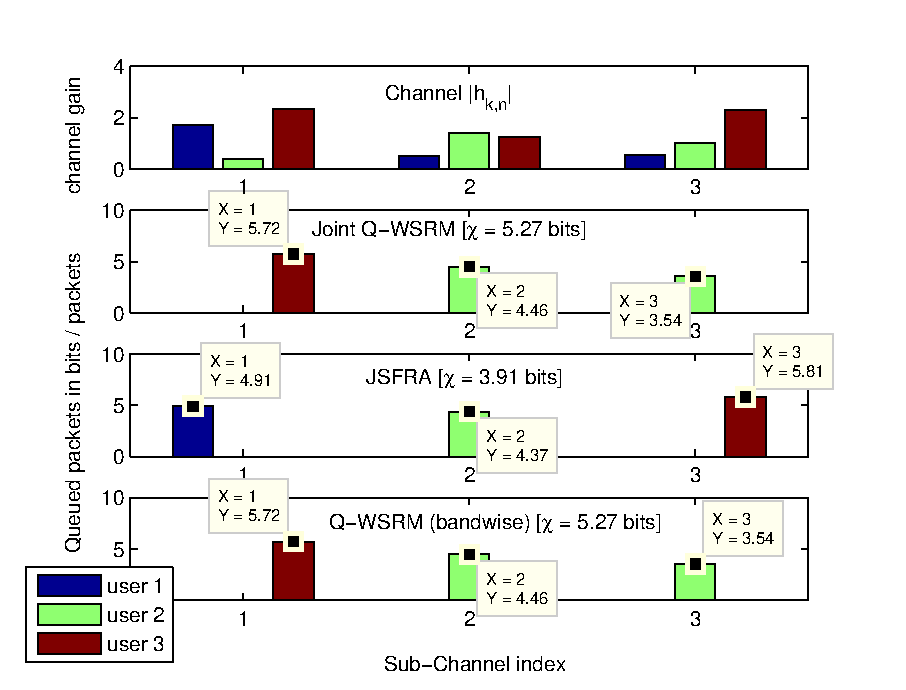
\includegraphics[width=\columnwidth]{tbl-1}
%\caption{Allocation for a \ac{SISO} Model comparing different Algorithms}
%\label{tbl-1}
%\end{figure}

In order to understand the behavior in a \ac{MIMO} framework, we consider a system with \me{N=3} sub-channels and \me{N_B = 3} \acp{BS}, each equipped with \me{N_T = 4} transmit antennas operating at \me{10}dB \ac{SNR}, serving \me{|\mc{U}_b| = 3} users each. The path loss between the \acp{BS} and the users are uniformly generated from \me{[0,-3]} dB and the association is made by selecting the \ac{BS} with lower path loss. Fig. \ref{fig-1} shows the performance of the centralized schemes for a single receive antenna system. It compares the total number of \ac{SCA} updates required by the \ac{JSFRA}, \ac{SRA} and the \ac{Q-WSRME} schemes to perform the optimal allocations to minimize the total number of backlogged packets.
\begin{figure*}
\centering
\subfloat[][System \me{\lbrace N,N_B,K,N_T,N_R \rbrace = \lbrace 4,3,9,4,1\rbrace}]{
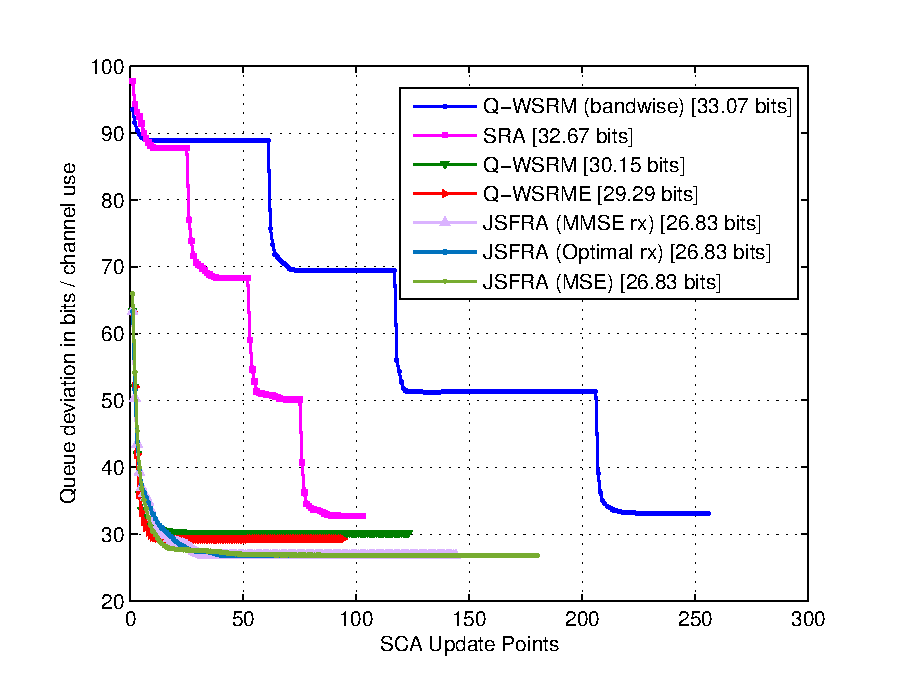
\includegraphics[width=0.48\textwidth]{fig-1-3}
\label{fig-1}}
\hfill
\subfloat[][System \me{\lbrace N,N_B,K,N_T,N_R \rbrace = \lbrace 3,3,9,4,2\rbrace}]{
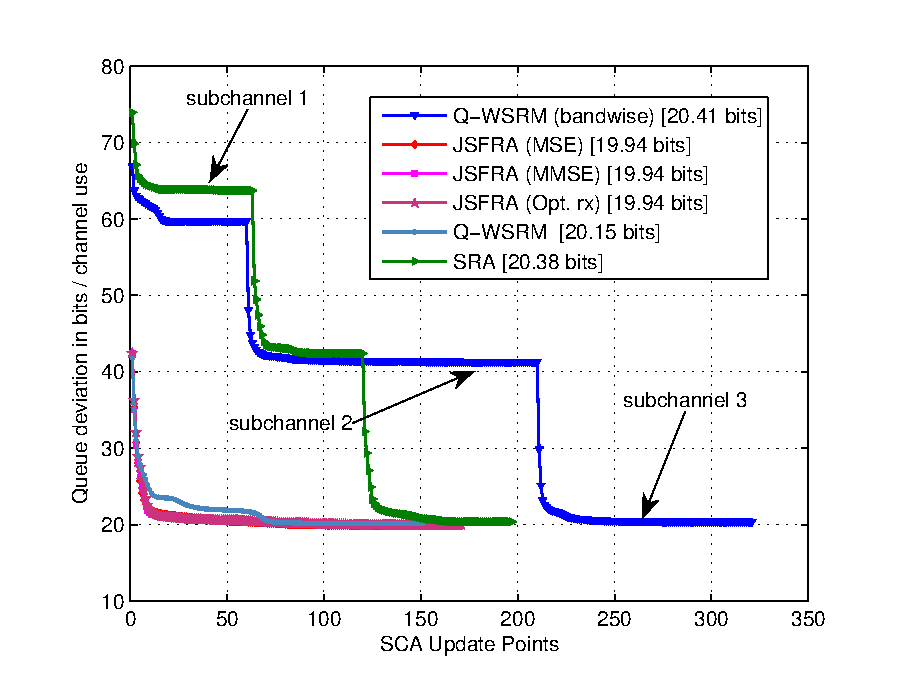
\includegraphics[width=0.48\textwidth]{fig-2-2}
\label{fig-2}}
\caption{Number of backlogged packets at the \ac{SCA} update points}
\label{fig-a}
\end{figure*}

In the sub-channel wise allocations, where the total transmit power is shared equally among the sub-channels, the precoders are designed for each sub-channels independently. In this approach, the precoders are coupled via the number of queued bits which are updated using \eqref{eqn-weight} before designing the precoders for the sub-channels. At each \ac{SCA} points, the number of queued bits are reduced significantly with the introduction of a new sub-channel since the algorithm starts with a random initial point before it converges to an optimal\footnote{due to the nonconvex nature of the original problem} precoders. The total number of backlogged bits at each \ac{SCA} update instant are plotted in Fig. \ref{fig-1} for the discussed centralized schemes and the convergence point are marked with the data tips. Fig. \ref{fig-2} compares the performance of the centralized algorithms for the \me{N_R = 2} receive antennas. In all the schemes, the receive beamformers are updated at the \ac{SCA} update points instead of updating after the \ac{SCA} convergence as in Algorithm. \ref{algo-1}. Since the receiver minimizes the objective for the fixed transmit precoders, the convergence is monotonic as can be seen from the figures.
\begin{table}
\centering
\renewcommand{\arraystretch}{1.25} \scriptsize
\begin{tabular}{|c|*{8}{c}|c|}
\hline
\me{q} & \multicolumn{8}{c|}{user indices} & \me{\chi} \\
\hline
\me{1} & 15.00 & 3.95 & 5.26 & 8.95 & 7.03 & 11.90 & 12.00 & 9.73 & 25.15 \\
\me{2} & 11.23 & 3.93 & 10.76 & 10.65 & 10.27 & 9.68 & 8.77 & 5.90 & 27.77 \\
\me{\infty} & 11.41 & 4.41 & 10.41 & 10.41 & 10.41 & 8.41 &  8.41 &  6.41 & 28.68 \\
\hline
\me{Q_k}  & 15.0 &  8.0 &  14.0 & 14.0 &  14.0 & 12.0 & 12.0 & 10.0  \\
\cline{1-9}
\end{tabular}
\caption{Queue information for the system \me{\lbrace N,N_B,K,N_R \rbrace = \lbrace 5,2,8,1 \rbrace}}
\label{tbl-3}
\end{table}
%\begin{figure}
%\centering
%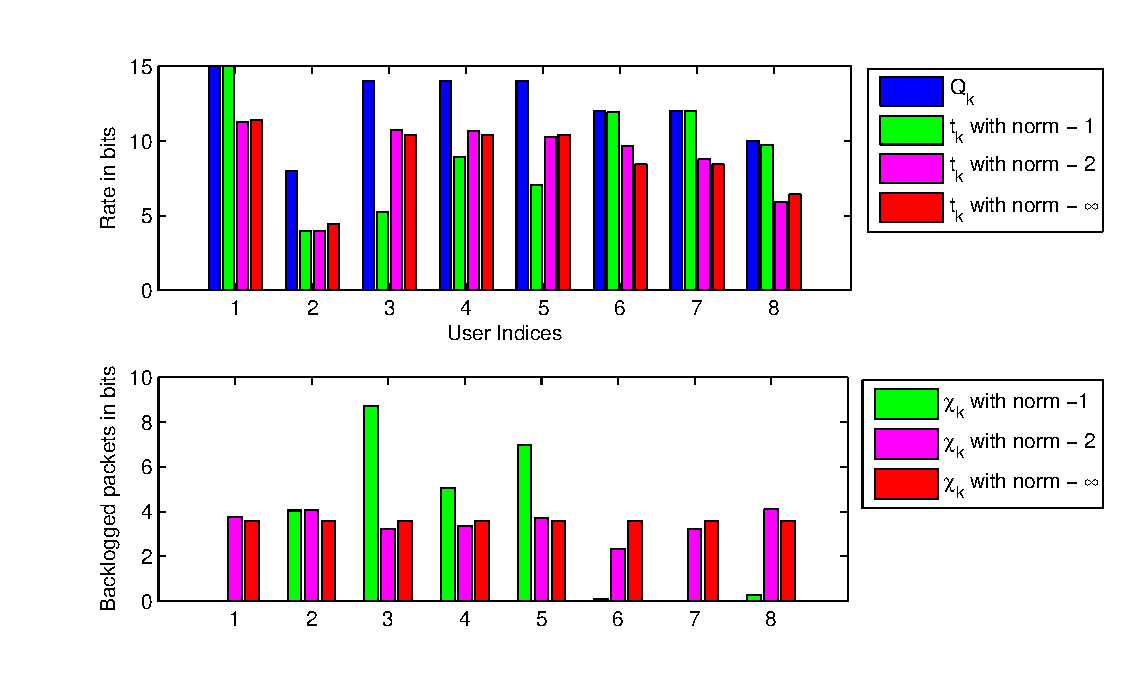
\includegraphics[width=\columnwidth]{tbl-2}
%\caption{Queue information for the system \me{\lbrace N,N_B,K,N_R \rbrace = \lbrace 5,2,8,1 \rbrace}}
%\label{tbl-3}
%\end{figure}

The behavior of the \ac{JSFRA} algorithm for different exponents \me{q} are outlined in the Table. \ref{tbl-3} for the users located at the cell-edge of the system employing \me{N_T = 4} transmit antennas. The configuration is mentioned in the caption of Table. \ref{tbl-3} along with the number of queued bits for each user. It is evident that the algorithm minimizes the queued bits for the \me{\ell_1} norm compared to the \me{\ell_2} norm, which is shown in the column displaying the total number of left over packets \me{\chi} in bits. The \me{\ell_{\infty}} norm provides fair allocation of the resources by making the left over packets to be equal for all users to \me{\chi_k = 3.58} bits. The \me{\ell_{\infty}} norm provides the fair allocation by making the queued deviation equal for all the users after the current allocation irrespective of their channel gains.


\subsection{Distributed Solutions} \label{sec-5.2}
The performance of the distributed algorithms are compared using the total number of backlogged packets after each \ac{SCA} update points. Fig. \ref{fig-d} compares the performance of the algorithms for the system configuration \me{\lbrace N,N_B,K,N_R \rbrace = \lbrace 3,2,8,1 \rbrace} with \me{N_T = 4} transmit antennas at the \acp{BS}. Each \ac{BS} serves \me{|\mc{U}_b| = 4} users in a coordinated manner to reduce the total number of backlogged packets at each \ac{BS}. The total number of queued packets assumed for both figures is \me{Q_k = [5,7,9,11,8,12,5,4]} bits. As pointed out in Section \ref{sec-4}, the performance and the convergence speed of the distributed algorithms are susceptible to the step size used in the subgradient update. Due to the fixed interference levels in the primal approach, it may lead to infeasible solutions if the initial or any intermediate update is not feasible.

Fig. \ref{fig-d} plots the performance of the primal and the \ac{ADMM} solutions for the \ac{JSFRA} scheme using the \ac{SCA} and by \ac{MSE} relaxation at each \ac{SCA} point. In between the \ac{SCA} updates, the primal or the \ac{ADMM} scheme is performed for \me{J_{\max} = 20} iterations to exchange the respective coupling variables. In Fig. \ref{fig-d}, the total number of backlogged packets at each \ac{SCA} points are plotted without the inner loop iterations of \me{J_{\max}} times for the primal or the dual variables convergence. It can be seen from Fig. \ref{fig-d} that the distributed algorithms approach the centralized performance by exchanging minimal information between the coordinating \acp{BS}.

\iftoggle{enable_dist_fig}
{	
In Fig. \ref{fig-d-2}, the performance of the distributed algorithms are studied for \me{K = 12} users utilizing \me{N = 6} sub-channels. The system considers \me{N_B = 3} \acp{BS}, each having \me{N_T = 4} transmit antennas serving \me{|\mc{U}_b| = 4} users equipped with \me{N_R = 2} antennas respectively. The users are assumed to have the path loss following the uniform distribution between \me{[0,-6]} dB from all \acp{BS}. The performance of the algorithms are similar to the \me{N_B = 2} \ac{BS} scenario discussed earlier.

Fig. \ref{fig-d-2} plots the performance of the centralized and the distributed algorithms at each \ac{SCA} update. In case of the distributed approaches, in between each \ac{SCA} update, the primal or the \ac{ADMM} exchanges are performed for \me{J_{\max} = 20} iterations. In practice, \me{J_{\max} = 1} can be set to perform the \ac{SCA} update, \ac{ADMM} or primal update, and the receive beamformers \me{\mvec{W}{k,n}} update at the same instant, which affects the convergence rate and the stationary point of the final solution. The data tips are used to highlight the convergent points of various algorithms. The performance of the \ac{JSFRA} schemes using the primal decomposition are notably inferior compared to the \ac{ADMM} approach for the same schemes. It is mainly attributed to the difficulty in selecting the step size for the system employing \me{N_B \geq 3} \acp{BS}.
\begin{figure*}[h]
	\centering
	\subfloat[][System \me{\lbrace N,N_B,K,N_R \rbrace = \lbrace 3,2,8,1 \rbrace}]{
		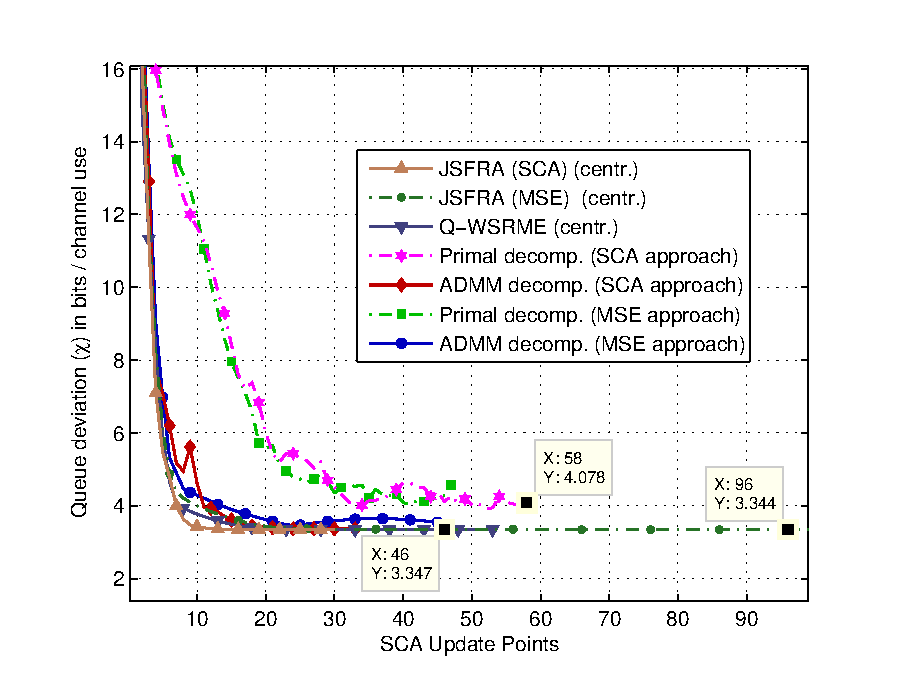
\includegraphics[width=0.48\textwidth]{fig-3-2}
		\label{fig-d-1}
	}
	\hfill
	\subfloat[][System \me{\lbrace N,N_B,K,N_R \rbrace = \lbrace 6,3,12,2 \rbrace}]{
		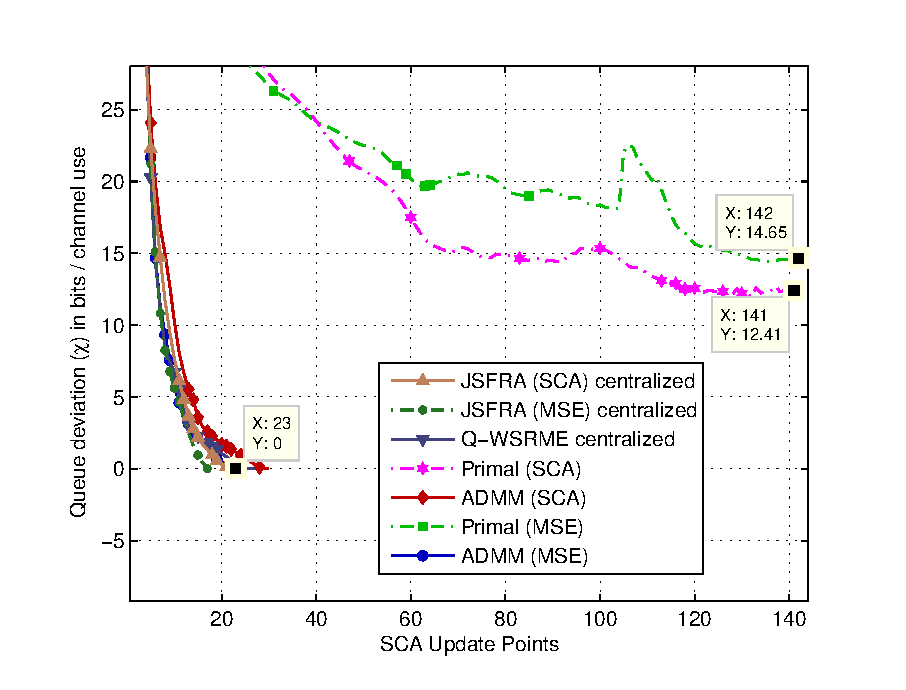
\includegraphics[width=0.48\textwidth]{fig-5-1}
		\label{fig-d-2}
	}
	\caption{Number of backlogged packets at each \ac{SCA} points}
	\label{fig-d}
\end{figure*}
% \begin{figure*}
% \centering
% \begin{subfigure}{0.49\textwidth}
% 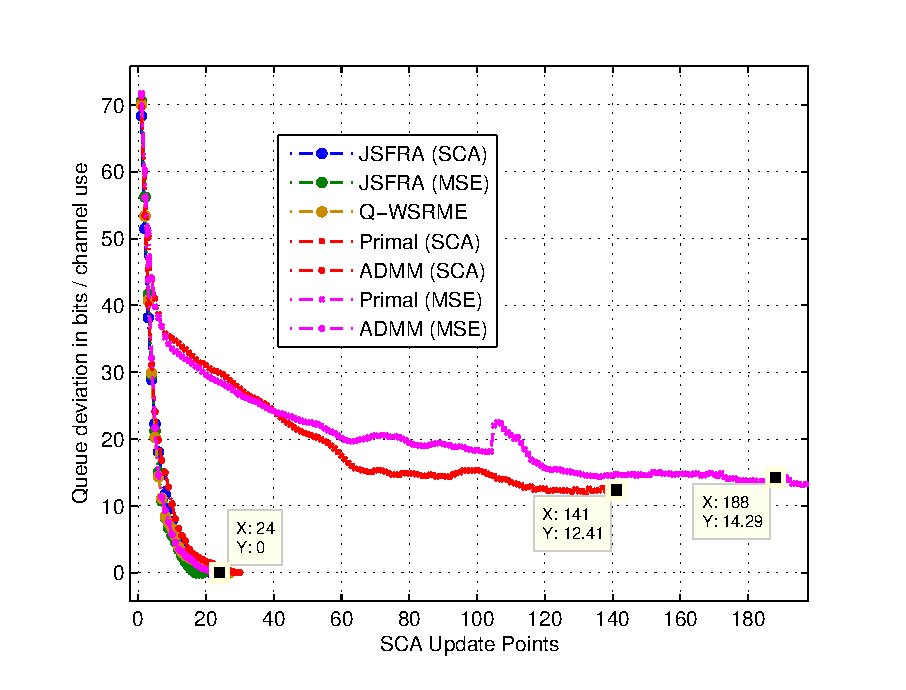
\includegraphics[width=\textwidth]{fig-5}
% \caption{Queue deviation}
% \end{subfigure}
% \hfill
% \begin{subfigure}{0.49\textwidth}
% 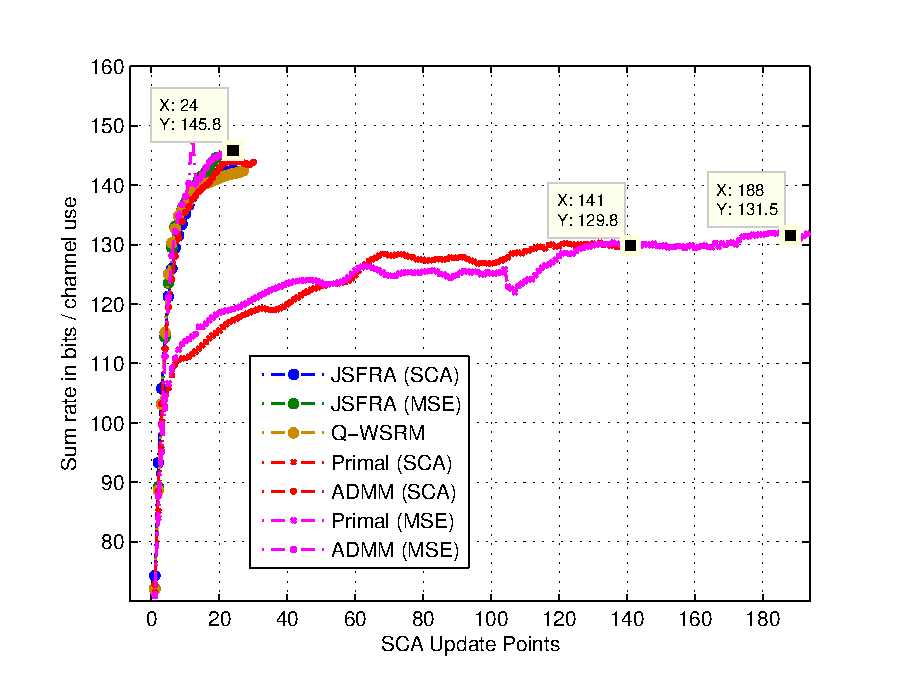
\includegraphics[width=\textwidth]{fig-6}
% \caption{Sum rate performance}
% \end{subfigure}
% \caption{Convergence plot for \me{\lbrace N,N_B,K,N_R \rbrace = \lbrace 6,3,12,2 \rbrace} model}
% \label{fig-d-2}
% \end{figure*}
}{
\begin{figure}[h]
\centering
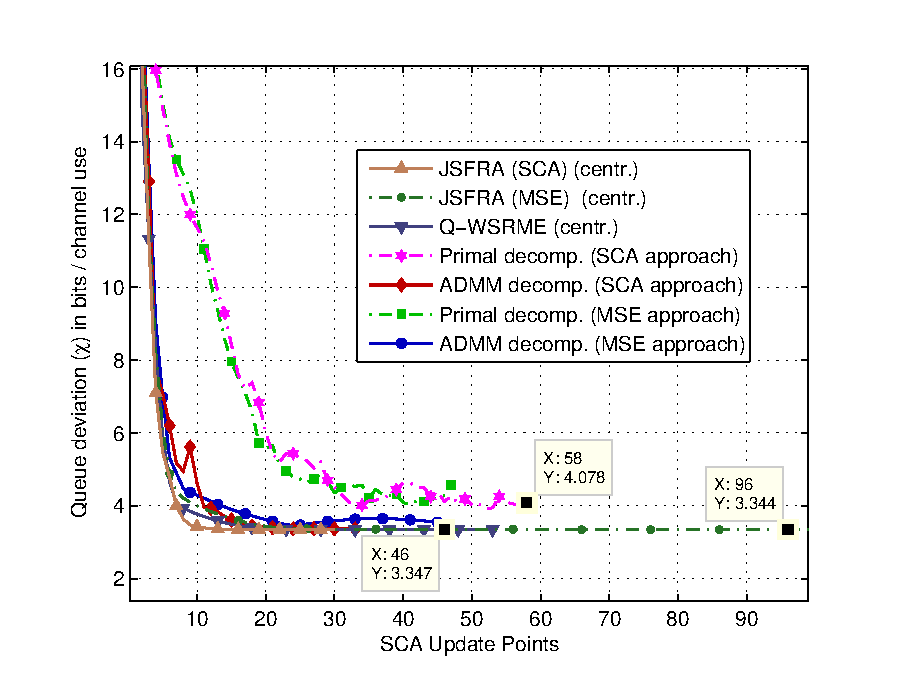
\includegraphics[width=\columnwidth]{fig-3-2}
\caption{Convergence behaviour of the centralized and the distributed algorithms for a system \me{\lbrace N,N_B,K,N_R \rbrace = \lbrace 3,2,8,1 \rbrace}}
\label{fig-d} \vspace{-0.1in}
\end{figure}
}
Fig. \ref{fig-d-3.1} compares the performance of the centralized and the \ac{KKT} algorithm in Section \ref{sec-4.3} for different exponents by plotting the total number of backlogged packets at each \ac{SCA} update point. The \me{\ell_1} norm \ac{JSFRA} scheme provides better performance over other schemes due to the greedy objective. The \ac{KKT} approach for \me{\ell_1} norm is not defined due to the non-differentiability of the objective as discussed in the Section \ref{sec-4.3}. If used for \me{\ell_1} norm, the problem of over-allocation will not affect the dual variables \me{\sigma_{l,k,n}} and \me{\alpha_{l,k,n}} since the queue deviation is raised to the power zero in \eqref{kkt-mse-4.2}, which will always be equal to one. A heuristic method based on subdifferential calculus in \cite{bertsekas1999nonlinear} is proposed in Fig. \ref{fig-d-3.1} by assigning zero for \me{\sigma_{l,k,n}} when the queue deviation is negative, \textit{i.e}, \me{Q_k - t_k < 0}. It is required to address the problem of over-allocation in the \me{\ell_1} norm for dropping the absolute value operator from the objective function. It can be seen that the heuristic method oscillates near the stationary point with the deviation determined by the factor \me{\rho} used in \eqref{kkt-mse-4.1}.
\begin{figure}
	\centering
	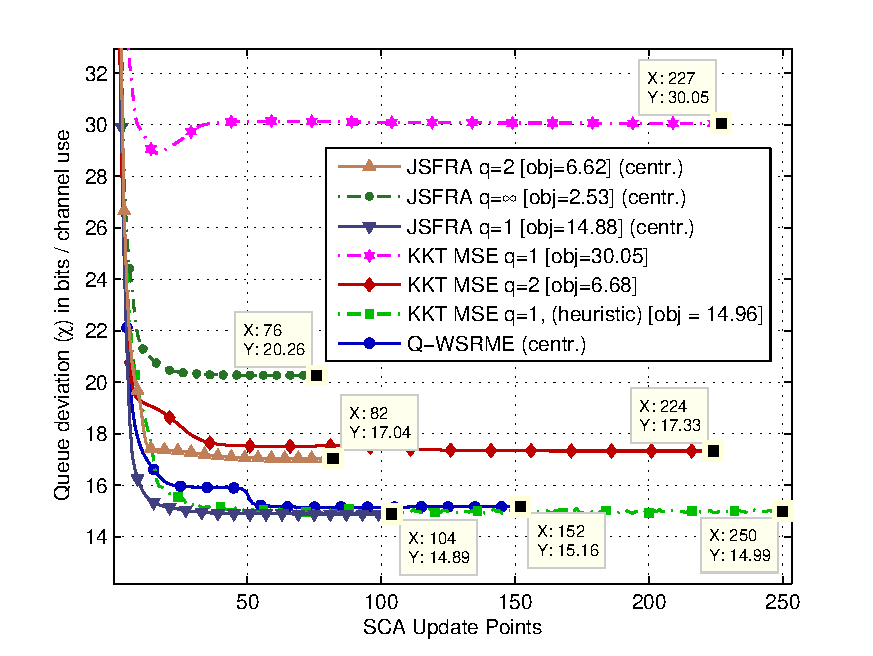
\includegraphics[width=\columnwidth]{fig-9-3}
	\caption{Impact of varying \me{q} in the total number of backlogged packets after each \ac{SCA} update for a system \me{\lbrace N,N_B,K,N_R \rbrace = \lbrace 5,2,8,1 \rbrace}}
	\label{fig-d-3.1} \vspace{-0.1in}
\end{figure}

The objective values are mentioned in the legend for all the schemes and the objective of the \me{\ell_2} norm is not the same as that of the \me{\ell_1} norm used for plotting. For simulations, we update all variables in \eqref{kkt-mse-4} at once at each iteration, \textit{i.e}, \me{J_{\max} = 1}, which is well justified for the practical implementations due to the signaling overheads. The \me{\ell_2} norm for the \ac{JSFRA} and the \ac{KKT} approach achieves nearly the same value of \me{6.62} with different \me{\chi}, due to the limited number of iterations for the dual variable convergence between each \ac{SCA} update. Fig. \ref{fig-d-3.1} also shows the effect of dropping the squared rate variable from the objective in the \ac{Q-WSRME} scheme compared to the \me{\ell_2} norm which includes it. By dropping it, the \ac{Q-WSRME} scheme minimizes the number of queued packets in a prioritized manner based on the respective queues. On contrary, the \me{\ell_2} norm allocate rates to the users with the higher number of queued packets before addressing the users with the smaller number of queued packets.




\subsection{Queuing Analysis over Multiple Transmission Slots} \label{time-correlated}

We discuss the performance of the \ac{JSFRA} algorithm for different \me{\ell_q} over multiple transmission slots. It is compared to the existing \ac{Q-WSRME} scheme by varying the average arrival rate \me{A_k} of all users. Fig. \ref{fig-time-analysis} plots the performances of the centralized algorithms for different \me{\ell_q} values. Even though \me{A_k}'s are constant for all users, the instantaneous arrivals are random and they follow the Poisson process. We considered a \me{4 \times 1} \ac{MIMO} with \me{N = 4} sub-channels and \me{N_B = 2} \acp{BS}. The \ac{PL} is modeled as a uniform random variable \me{[0,-3]} dB.

Fig. \subref*{fig-review} compares various schemes with the average number of backlogged packets present in the system after each transmission slot. The performance of the \ac{JSFRA} scheme using \me{\ell_2} is similar to the \ac{Q-WSRME} approach in the average number of residual packets after each transmission slot. Note that the additional rate constraints in the \ac{Q-WSRME} scheme is the reason for the equivalence. Both \ac{Q-WSRM} and \ac{Q-WSRME} performs similar to \me{\ell_2} \ac{JSFRA} scheme when the arrival rates are larger than those of the actual transmissions. Fig. \ref{fig-time-analysis} shows that the number of backlogged packets are noticeably less for the \me{\ell_1} \ac{JSFRA} scheme due to the greedy allocation of serving users with better channel. Fig. \ref{fig-time-analysis} highlights that the \me{\ell_{\infty}} \ac{JSFRA} scheme performs equally well compared to the other objectives when the system is in the stable region. On contrary, the performance is inferior in the unstable region, since the fair allocation is not effective when the number of backlogged packets is large for all users.


%acresetall
\section{Conclusions} \label{sec-6}
In this paper, we addressed the problem of allocating downlink space-frequency resources to the users in a multi-cell \ac{MIMO} \ac{IBC} system using \ac{OFDM} transmission. The resource allocation is considered as a joint space-frequency precoder design problem since the allocation of a resource to a user is obtained by a non-zero precoding vector. We proposed the \ac{JSFRA} scheme by employing the \ac{SCA} technique to relax the nonconvex constraint by a sequence of convex subsets for designing the precoders to minimize the total number of user queued packets. Additionally, an alternative \ac{MSE} relaxation approach is also proposed by using \ac{SCA} technique to address the nonconvex constraints for a fixed \ac{MMSE} receivers. We then introduced distributed precoder designs for the \ac{JSFRA} problem using primal and \ac{ADMM} methods. Finally, we proposed a practical iterative algorithm to obtain the precoders in a decentralized manner by solving the \ac{KKT} conditions of the \ac{MSE} reformulated \ac{JSFRA} method. The proposed iterative algorithm requires few iterations and limited signaling exchange between the coordinating \acp{BS} to obtain the efficient precoders for a given number of iterations. Numerical results are provided to compare the performance of the proposed algorithms with the existing solutions.

\appendices

%\section{\acl{PD} approach} \label{a-2}
%By fixing the interference values \me{\zeta_{\pr{l},\pr{k},n,{b_k}}} corresponding to the interference from the \ac{BS} \me{b_k}, the constraint involving the coupling variables \eqref{eqn-9.1c} can be relaxed using the equivalent formulation in \eqref{eqn-decent-3}. Now, the subproblem for the \ac{BS} \me{b_k \in \mc{B}} can be obtained by grouping the terms relevant to the \ac{BS} \me{b_k} as
\begin{IEEEeqnarray}{rCl} \label{eqn-primal-1}
\underset{\substack{\gamma_{l,k,n} \\ \mvec{m}{l,k,n}, \beta_{l,k,n}}}{\text{minimize}} &\quad & \| \tilde{\mbf{v}}_{b_k} \|_q \IEEEyessubnumber \label{eqn-primal-1a} \\
\text{subject to}&\quad&\sum_{n = 1}^N \sum_{k \in \mathcal{U}_{b_k}} \text{tr} \, (\mvec{M}{k,n} \mvec{M}{k,n}^\herm) \leq P_{{\max}}, \IEEEyessubnumber \label{eqn-primal-1c} \\
&& \beta_{l,k,n} \geq \sum_{\substack{j = 1\\j \neq l}}^L |\mvec{w}{l,k,n}^\herm \mvec{H}{{b_k},k,n} \mvec{m}{j,k,n} |^2 \nonumber \\
&&\quad + \sum_{i \in \mc{U}_{b_k} \backslash \{k\}} \sum_{j = 1}^L |\mvec{w}{l,k,n}^\herm \mvec{H}{{b_k},k,n} \mvec{m}{j,i,n} |^2 + \sum_{b \in \bar{\mc{B}}_{b_k}} \zeta_{l,k,n,b} \; + \; N_0\|\mvec{w}{l,k,n}\|^2 \IEEEyessubnumber \label{eqn-primal-1d} \\
&& \zeta_{\pr{l},\pr{k},n,{b_k}} \geq \sum_{k \in \mc{U}_b} \sum_{l = 1}^L |\mvec{w}{\pr{l},\pr{k},n}^\herm \mvec{H}{b_k,\pr{k},n} \mvec{m}{l,k,n} |^2, \; \forall \pr{k} \in \bar{\mc{U}}_{b_k}, \; \forall n \in \mc{C} \IEEEyessubnumber \label{eqn-primal-1e} \\
 & \quad & \text{and} \; \eqref{eqn-8} \IEEEyessubnumber,
\end{IEEEeqnarray}

Let \me{\mbfa{\zeta}^{\set{b_k}}} be the vector representing the fixed interference levels relevant to the \ac{BS} \me{b_k} in a fully connected network\footnote{in practice it will be less due to the path loss}, which is given by
\begin{IEEEeqnarray}{RCL} \label{eqn-primal-2}
\mbfa{\zeta}_{k,n,b} &=& \left [ \; \zeta_{1,k,n,b}, \dotsc, \zeta_{L,k,n,b} \; \right ] \IEEEyessubnumber \\
\mbfa{\zeta}^{\set{b_k}}_n &=& \left [ \; \mbfa{\zeta}_{\mc{U}_{b_k}(1),n,\bar{\mc{B}}_{b_k}(1)}, \dotsc, \mbfa{\zeta}_{\mc{U}_{b_k}(1),n,\bar{\mc{B}}_{b_k}(|\bar{\mc{B}}_{b_k}|)}, \right . \nonumber \\
&& \left . \dotsc, \mbfa{\zeta}_{\mc{U}_{b_k}(|\mc{U}_{b_k}|),n,\bar{\mc{B}}_{b_k}(|\bar{\mc{B}}_{b_k}|)}, \dotsc, \mbfa{\zeta}_{\bar{\mc{U}}_{b_k}(1),n,b_k}, \dotsc, \mbfa{\zeta}_{\bar{\mc{U}}_{b_k}(|\bar{\mc{U}}_{b_k}|),n,b_k} \; \right  ] \IEEEyessubnumber \\
\mbfa{\zeta}^{\set{b_k}} &=& \left [ \; \mbfa{\zeta}^{(b_k)}_1, \dotsc, \mbfa{\zeta}^{(b_k)}_N \; \right ], \IEEEyessubnumber
\end{IEEEeqnarray}
where the length of the vector \me{\mbfa{\zeta}^{\set{b_k}}} is
\begin{equation}
n_{b_k} = | \mbfa{\zeta}^{\set{b_k}} | = \left ( |\bar{\mc{B}}_{b_k}| |\mc{U}_{b_k}| + |\bar{\mc{U}}_{b_k}|\right ) L N
\label{primal-vec-len}
\end{equation}

The local subproblem \eqref{eqn-primal-1} solved at each \ac{BS} are coordinated by the master problem, which updates the interference thresholds \me{\mbfa{\zeta}^{\set{b}}, \forall b \in \mc{B}} for the next iteration. The master problem controlling multiple subproblems is given by
\begin{IEEEeqnarray}{rCl} \label{eqn-primal-3}
\underset{\mbfa{\zeta}}{\text{minimize}} & \quad & \sum_{b \in \mc{B}} \alpha^{\star}_b (\mbfa{\zeta}^{\set{b}}) \IEEEyessubnumber \\
\text{subject to} & \quad & \mbfa{\zeta}^{\set{b}} \in \mathbb{R}_+^{n_b}, \forall b \in \mc{B}, \IEEEyessubnumber
\end{IEEEeqnarray}
where \me{\alpha^{\star}_b (\mbfa{\zeta}^{\set{b}})} denotes the optimal solution for \eqref{eqn-primal-1} with the previous value of \me{\mbfa{\zeta}^{(i-1)}}, where \me{\mbfa{\zeta}} is the global interference vector formed by stacking the interference vector associated with each \ac{BS} as \me{\mbfa{\zeta} = \left [ \mbfa{\zeta}^{\set{\mc{B}(0)}}, \mbfa{\zeta}^{\set{\mc{B}(1)}}, \ldots, \mbfa{\zeta}^{\set{\mc{B}(|\mc{B}|)}}\right ]}.

The master problem to find the optimal \me{\mbfa{\zeta}^{\set{b_k}(i)}, \forall b_k \in \mc{B}} is given by the following subgradient method \cite{bertsekas1999nonlinear} as
\begin{equation} \label{primal-sg-update}
\zeta^{\set{b_k}(i)}_{l,k,n,b} = \left [\zeta_{l,k,n,b}^{\set{b_k}(i-1)} - \rho \, s_{l,k,n,b}^{\set{b_k}(i-1)} \right ]^+, \forall b \in \mc{B}, \forall k \in \bar{\mc{U}}_b,
\end{equation}
where \me{i} is the iteration index, \me{\rho} is the positive step size, and \me{s^{\set{b_k}(i-1)}_{l,k,n,b}} is the subgradient of the problem defined in \eqref{eqn-primal-3} evaluated at \me{\zeta^{(i-1)}_{l,k,n,b}}. To find the subgradient \me{s^{\set{b_k}(i-1)}_{l,k,n,b}}, the dual variables corresponding to the interference constraints are required, which can be obtained by forming the dual problem of \eqref{eqn-primal-2} as discussed in \cite{pennanen2011decentralized}. Now the primal and the dual variables \me{\mu^{\set{b_k}}_{l,k,n}} and \me{\mu^{\set{b_k}}_{\pr{l},\pr{k},n}} corresponding to the constraints \eqref{eqn-primal-1d} and \eqref{eqn-primal-1e} can be obtained from the solvers, which solves the dual problem as well.

To obtain the next interference iterate at each \ac{BS}, the locally evaluated dual variables are exchanged among the \acp{BS} in the set \me{\mc{B}} in order to obtain the next interference vector in a distributed manner. Once we obtain the dual variables from all the \acp{BS}, the subgradients relevant to the \ac{BS} \me{b_k} are evaluated by taking the difference between the two \acp{BS} associated with each interference value, \textit{i.e}, \me{s^{\set{b_k}(i)}_{l,k,n,b} = \mu^{\set{b_k}}_{l,k,n} - \mu^{\set{b}}_{l,k,n}}. With the newly estimated subgradient value \me{s^{\set{b_k}(i)}_{l,k,n,b}}, the interference terms corresponding to the \ac{BS} \me{b_k} are updated using \eqref{primal-sg-update}. The algorithmic representation of the \ac{PD} approach is detailed in Algorithm. \ref{algo-2}.
\begin{algorithm}
 \SetAlgoLined
 \DontPrintSemicolon
 \BlankLine
 \SetKwInput{KwInit}{Initialize}
 \KwIn{\me{a_k, \, Q_k, \, \mvec{H}{b,k,n},\; \fall b \in \mathcal{B}, \, \fall k \in \mathcal{U}, \fall n \in \mathcal{C}}}
 \KwOut{\me{\mvec{m}{l,k,n}} and \me{\mvec{w}{l,k,n} \fall l \in \set{1,2,\dotsc,L}}}
 \KwInit{\me{i=0} and the transmit precoders \me{\tilde{\mbf{m}}_{l,k,n}} randomly satisfying the total power constraint \eqref{eqn-4.3}}
 update \me{\mvec{w}{l,k,n}} with \eqref{eqn-10} and \me{\tilde{\mbf{u}}_{l,k,n}} with \eqref{eqn-8} using \me{\tilde{\mbf{m}}_{l,k,n}} \;
 initialize the interference threshold \me{\zeta_{l,k,n,b}^{\set{0}} \forall b \in \mc{B}, \forall k \in \bar{\mc{U}}_{b_k}, \forall l,n} \;
 for each \ac{BS} \me{b \in \mc{B}}, perform the following procedure \;
 \Repeat{convergence or \me{i \geq I_{\max}}}{
    initialize \me{j=0} \;
    \Repeat{convergence or \me{j \geq J_{\max}}}{
        solve for the transmit precoders \me{\mvec{m}{l,k,n}} and dual variables \me{\mu^{\set{b}}_{l,k,n}} using \eqref{eqn-primal-2} \;
        exchange \me{\mu^{\set{b}}_{l,k,n}} across the coordinating \acp{BS} in \me{\mc{B}} \;
        update \me{\zeta^{\set{b}(j+1)}_{l,k,n,b}} using \eqref{primal-sg-update} locally \;
        \me{j = j + 1} \;
    }
    update the receive beamformers \me{\mvec{w}{l,k,n}} using \eqref{eqn-10} with the recent precoders \me{\mvec{m}{l,k,n}} \;
    exchange the receive precoders \me{\mbf{W}_{k,n}} \me{\forall k \in \mc{U}_b} among the \acp{BS} in \me{\mc{B}} \;
    update \me{\tilde{p}_{l,k,n}}, \me{\tilde{q}_{l,k,n}} and \me{\tilde{\beta}_{l,k,n}} with the recent precoders using \eqref{eqn-wsrm-expr} and \eqref{eqn-6.3} for the \ac{SCA} approach (or) \;
    update \me{\tilde{\epsilon}_{l,k,n}} with the recent precoders using \eqref{eqn-mse-2.3} with equality for the \ac{MSE} formulation approach \;
    $i = i + 1$ \;
  }
 \caption{Decentralization via Primal Decomposition for \acs{JSFRA} scheme}
  \label{algo-2}
\end{algorithm}


%\section{Tightness of \ac{SINR} relaxation} \label{a-3}
%\begin{comment}
For the constraints \eqref{eqn-6.2} and \eqref{eqn-6.3} to be active, there should be at least one user in each \ac{BS} with enough backlogged packets that cannot be served with the given power budget. To prove this, let us consider a \ac{BS} \me{b} with \me{N_T \times 1} system serving \me{|U|_b} users each with \me{Q_k} backlogged packets. The \ac{JSFRA} formulation can be written as
\begin{IEEEeqnarray}{rCl} \label{tight}
	\underset{\gamma_{k},\mvec{m}{k},\beta_{k}}{\text{minimize}} &\quad& \sum_{k \in \mc{U}_b} \big | Q_k - \log_2(1 + \gamma_k) \big |^q  \eqsub \\
	\text{subject to} &\quad& \gamma_{k} \leq \frac{ | \mvec{H}{k} \mvec{m}{k}|^2}{\beta_{k}} \IEEEyessubnumber \label{ae-1} \\
	&\quad& \beta_{k} \geq N_0 + \sum_{\mathclap{i \neq k}} |\mvec{H}{k} \mvec{m}{i} |^2 \IEEEyessubnumber \label{ae-2} \\
	&\quad& \sum_{k \in \mc{U}_b} \trace \, (\mvec{m}{k} \mvec{m}{k}^\herm) \leq P_{{\max}}. \IEEEyessubnumber \label{ae-3}
\end{IEEEeqnarray}
Let \me{N_T > |\mc{U}_b|} and the precoders are found by solving \eqref{tight} with a nonzero objective value at the optimal point. Let us consider two users, say \me{i} and \me{j} with precoders \me{\mvec{m}{i}} and \me{\mvec{m}{j}}. In order to show the tightness of \eqref{ae-1} and \eqref{ae-2}, let us assume by contradiction that \eqref{ae-1} and \eqref{ae-2} are not tight for user \me{i} only. Let us also consider that \me{\gamma_k} for all users \me{k \in \mc{U}_b \backslash j} are identified to satisfy the backlogged packets. 

Now, in order to minimize the objective of the \me{\ith{i}} user, \me{\gamma_i} should be \me{2^{Q_i} - 1} to have the minimum objective. Since the constraints \eqref{ae-1} and \eqref{ae-2} are not tight for the \me{\ith{i}} user, the actual \ac{SINR} on the r.h.s of \eqref{ae-1} is greater than \me{\gamma_i}. It is attributed to the excess power in the transmit precoder of user \me{i} as \me{\mvec{m}{i} = \bar{\mbf{m}}_{i} + \mbf{V}_i \mbf{e}}, where \me{\mvec{V}{i} = \mc{N}([\mbf{H}^{\mathrm{T}}_0, \dotsc, \mbf{H}^{\mathrm{T}}_{i-1},\mbf{H}^{\mathrm{T}}_{i+1}, \dotsc,\mbf{H}^{\mathrm{T}}_{|\mc{U}_b| - 1}]^{\mathrm{T}})} denotes the null space corresponding to the other user channel vectors and \me{\mbf{e}} be any random vector with power \me{\Delta P}. Note that the extra power has no impact on the interference constraint \eqref{ae-2} of other users. 

Since the allocated rate of user \me{j} is less than the queued packets, we can find a precoder \me{\mvec{m}{j}} with the additional power of \me{\Delta P} as \me{\mvec{m}{j}^\prime = \bar{\mbf{m}}_{j} + \mvec{V}{j} \mbf{e}^\prime}. Note that the new precoder has no impact on the interference constraint of other users. The newly found precoder \me{\mvec{m}{j}^\prime} minimize the queue of user \me{j} without affecting the rates of other user, there by reduces the objective further. It is in contradiction to our original assumption that the precoders are optimal and the objective is minimum. 

It can be seen that the constraints are tight as long as there is one user with unserviced backlogged packets at each \ac{BS} with the given power budget. Since the objective is not to minimize power, when the power budget is more than sufficient to service the backlogged packets of all users, the \ac{JSFRA} scheme is not guaranteed to find the minimum power precoders to empty the current backlogged packets in the system. The objective of the \ac{JSFRA} problem can be regularized by including the power term to find the minimum power precoders as
\begin{equation*}
\| \tilde{\mbf{v}} \|_q + \varphi \sum_{k \in \mc{U}} \sum_{n = 1}^{N} \sum_{l=1}^{L} \mathrm{tr} \left ( \mvec{m}{l,k,n} \mbf{m}^\herm_{l,k,n} \right ),
\end{equation*}
for a small \me{\varphi} without affecting the optimal solution. Note that the above objective is guaranteed to make the constraints \eqref{eqn-6.2} and \eqref{eqn-6.3} active by relaxing the power constraint \eqref{eqn-6.4}.
\end{comment}

For the constraints \eqref{eqn-6.2} and \eqref{eqn-6.3} to be active, there should be at least one user in each \ac{BS} with enough backlogged packets that cannot be served with the given power budget. In order to make the constraints active for all scenarios, the objective of the \ac{JSFRA} formulation should be regularized with the transmit power without affecting the solution as
\begin{equation*}
\| \tilde{\mbf{v}} \|_q + \varphi \sum_{k \in \mc{U}} \sum_{n = 1}^{N} \sum_{l=1}^{L} \mathrm{tr} \left ( \mvec{m}{l,k,n} \mbf{m}^\herm_{l,k,n} \right ),
\end{equation*}
where \me{\varphi \approx 0}. Note that the modified objective will relax the power constraint by making the constraints \eqref{eqn-6.2} and \eqref{eqn-6.3} active at the stationary point.



\section{Convergence Proof for Centralized Algorithm} \label{sec-3.5}
The following conditions are required to show the convergence of Algorithm \ref{algo-1}, which is used to solve problems \eqref{eqn-6} and \eqref{eqn-mse-1} in an iterative manner.
\begin{itemize}
	\item[(a)] Objective function should be bounded below
	\item[(b)] Feasible set should be compact
	\item[(c)] Sequence of objective values should be strictly decreasing
	\item[(d)] Uniqueness of the minimizer in each step.
\end{itemize}
\review{The conditions (a), (b), and (c) are required to prove the convergence of objective sequence generated by Algorithm \ref{algo-1}. However, to ensure strict monotonicity of the objective sequence, we require condition (d). Therefore, by assuming (a), (b), and (c) are satisfied by Algorithm \ref{algo-1}, the convergence of the objective sequence can be shown by using \cite[Th. 3.14]{rudin1964principles}. Finally, by using the discussions in \cite{marks1978technical,lanckriet2009convergence,scutari_1}, we show that \reviewF{every limit point of the sequence of iterates generated by Algorithm \ref{algo-1} is a stationary point of nonconvex problems \eqref{eqn-6} and \eqref{eqn-mse-1}}. The term iterates denotes the stacked vector of solution variables obtained in each iteration.}

Before discussing the convergence analysis, let us consider a generalized formulation for the problems in \eqref{eqn-6} and \eqref{eqn-mse-1} as
\begin{IEEEeqnarray}{RcL} \label{con} \neqsub
	\underset{\mx,\my,\mz}{\text{minimize}} &\quad& \hat{f}(\mx,\my,\mz) \eqsub \label{con-obj} \\
	\text{subject to} &\quad& h(\mz) - g_0(\mx,\my) \leq 0 \eqsub \label{con-dc} \\
	&\quad& g_1(\mx,\my) \leq 0 \eqsub \label{con-cvx-blk} \\
	&\quad& g_2(\mx) \leq 0 \eqsub \label{con-cvx}
\end{IEEEeqnarray}
where the functions \me{g_2} and \me{\hat{f}} are convex, and the function \me{h} is linear. Let functions \me{g_0} and \me{g_1} be convex w.r.t either \me{\mx} or \me{\my}, but not jointly convex on both variables. The constraint \eqref{con-dc} corresponds to \eqref{eqn-6.2} or \eqref{eqn-mse-1.2} and the constraint \eqref{con-cvx-blk} corresponds to \eqref{eqn-6.3} or \eqref{eqn-mse-1.3} respectively. Other convex constraints are handled by \eqref{con-cvx} and the feasible set of \eqref{con} is given by 
\iftoggle{single_column}{
	\begin{equation}
		\mc{F} = \{ \; \mx,\my,\mz \; \big | h(\mz) - g_0(\mx,\my) \leq 0, g_1(\mx,\my) \leq 0, g_2(\mx) \leq 0 \}.
	\end{equation}
}{\begin{align}
\mc{F} = \{ \; \mx,\my,\mz \; \big | & \quad h(\mz) - g_0(\mx,\my) \leq 0, \nonumber \\
& \quad g_1(\mx,\my) \leq 0, g_2(\mx) \leq 0 \}.
\end{align}}

\review{We use the following notations to discuss the convergence proof. Since Algorithm \ref{algo-1} involves two nested iterations, \textit{i.e.}, one for \ac{SCA} and another one for \ac{AO}, we denote \ac{AO} step by a superscript \me{(i)} and \ac{SCA} iteration by a subscript \me{k}. Let \me{\mx}, \me{\my}, and \me{\mz} be the stacked vector all transmit precoders, receive beamformers, and other optimization variables present in the formulations \eqref{eqn-6} and \eqref{eqn-mse-1} respectively. Since Algorithm \ref{algo-1} includes two \ac{SCA} iterations performed until convergence in each \ac{AO} iteration, let us now consider \ac{AO} step \eqn{i} for fixed \eqn{\my}. The solution obtained at the \eqn{\ith{k}} \ac{SCA} step is represented as \eqn{\mx=\iter{\mx}{k}{i}} and \eqn{\mz=\iter{\mz}{k}{i}}. As \eqn{k \rightarrow \infty}, the objective sequence converges, and the corresponding solution obtained is denoted as \me{\iter{\mx}{\lpointx}{i}} and \me{\iter{\mz}{\lpointx|\my}{i}}. Similarly, for fixed \eqn{\mx} and as \eqn{k \rightarrow \infty}, the corresponding solution obtained is represented as \me{\my = \iter{\my}{\lpointx}{i}} and \me{\mz = \iter{\mz}{\lpointx|\mx}{i}} respectively.}

%We denote \me{\iter{\mx}{\lpointx}{i}} and \me{\iter{\mz}{|\my}{i}} as the solution obtained for \me{\mx} and \me{\mz} when the sequence of objective values converges in \eqn{\ith{i}} \ac{AO} step for fixed \eqn{\my}. Similarly, \me{\iter{\my}{\lpointx}{i}} and \me{\iter{\mz}{|\mx}{i}} correspond to the solutions of \eqn{\my} and \eqn{\mz} in \eqn{\ith{i}} \ac{AO} update for fixed \eqn{\mx}.

\subsection{Bounded Objective Function and Compact Feasible Set} \label{b_obj}
The feasible sets of the problems \eqref{eqn-6} and \eqref{eqn-mse-1} are bounded and closed, which is due to the total power constraint on the transmit precoders \eqref{eqn-6.4}, therefore, the sets are compact. 

The minimum of the norm in the objective is \me{\|x\|_q > -\infty}, therefore, it is bounded below. The objective function is Lipschitz continuous over the feasible set. The objective function is bounded from above as well, since the feasible set is bounded. %The objective function in \eqref{eqn-6} and \eqref{eqn-mse-1} is continuous and approaches \me{\infty} as \me{\mbf{t}_k \rightarrow \infty}, and therefore it is coercive in the feasible set. %Using conditions (a) and (b), we can guarantee the existence of a minimizer to the problem in \eqref{eqn-6} and \eqref{eqn-mse-1}.

\subsection{Uniqueness of the Iterates and Strong Convexity} \label{c-a}
%The uniqueness of the iterates \eqn{\{\iter{\mx}{k}{i},\iter{\my}{\lpointx}{i-1},\iter{\mz}{k|\my}{i}\}} can be ensured for the \ac{MSE} reformulated problem in \eqref{eqn-mse-2} when all the constraints are active. However when \eqn{\hat{f}(\iter{\mx}{k}{i},\iter{\my}{\lpointx}{i-1},\iter{\mz}{k|\my}{i}) = 0} after some iteration, say \me{k} and \me{i}, the uniqueness cannot be guaranteed as there can be multiple solutions with the same objective value in the feasible set. Similarly, when the objective is non-zero for \eqref{eqn-9}, the minimizer is unique only if the receivers are matched to the transmit beamformers. %, \textit{i.e.}, \me{q_{l,k,n} = 0} in \eqref{eqn-wsrm-expr}, while initializing the feasible point \eqn{\iter{\mx}{0}{0}} and \eqn{\iter{\my}{0}{0}}.

To ensure the uniqueness of the transmit and the receive beamformers, the objective function of the convex subproblems in \eqref{eqn-9} and \eqref{eqn-mse-2} are regularized by a strongly convex function in each \ac{SCA} iteration \eqn{k} and \ac{AO} update step \eqn{i} as 
\begin{IEEEeqnarray}{rCl} \neqsub
	\hat{f}(\mbf{z}) &=& \| \tilde{\mbf{v}} \|_q \eqsub \label{orig_obj} \\ 
	f(\mbf{z}) &=& \hat{f}(\mbf{z}) + {\tau}_k^{(i)} \, \| \mbf{z} - \mbf{z}^{(i)}_{k} \|^2_2 \eqsub \label{mod_obj} 
\end{IEEEeqnarray}
where \eqn{\mbf{z}} is a vector stacking all optimization variables, which can be either \eqn{[\mx,\iter{\my}{\lpoint}{i-1},\mz]} or \eqn{[\iter{\mx}{\lpoint}{i},\my,\mz]} depending on the problem and \eqn{\mbf{z}^{(i)}_{k} \triangleq [\mx_{k}^{(i)},\iter{\my}{\lpoint}{i-1},\mz_{k}^{(i)}]} is the solution obtained in the previous \eqn{\ith{(k-1)}} \ac{SCA} step. The positive constant \me{{\tau}_{k}^{(i)} > 0} ensures the strong convexity of \eqn{f} in each step and \eqn{c > 0} be the constant of strong convexity, defined as \eqn{c \triangleq \min_{k} \{{\tau}_{k}^{(i)}\}}, as shown in \cite{scutari-1}. Thus, due to the strong convexity of \eqn{f} in \eqref{mod_obj}, uniqueness of the minimizer is guaranteed in each \ac{SCA} step as discussed in \cite{yang_yang,scutari-1}. 

%in each step and let \eqn{c > 0} be the constant of strong convexity of \eqn{f} with \eqn{c \triangleq \min_{k} \{{\tau}_{k}^{(i)}\}} as in \cite{scutari-1}.
%The uniqueness of the transmit precoders and the receive beamformers for the \ac{MSE} reformulation in \eqref{eqn-mse-2} can be guaranteed in each iteration by the \ac{MSE} constraint in \eqref{eqn-mse-1.3}. The uniqueness of the iterates for the problem in \eqref{eqn-9} can be guaranteed in each convex subproblem if the receivers are matched to the equivalent downlink channel with the initially chosen feasible transmit precoders, \textit{i.e.}, \me{q_{l,k,n} = 0 \: \forall \, l,k,n} in \eqref{eqn-wsrm-expr} while beginning the \ac{SCA} iteration.
%of the objective
%When the objective is zero, the uniqueness of  the transmit and the receive beamformers are not guaranteed in both problem formulations, since they are the under-estimators and need not be active at the minimum. To obtain a unique set of transmit precoders and the receive beamformers in all scenarios, we can regularize the objective with a strongly convex function as
%\begin{equation}
%\| \tilde{\mbf{v}} \|_q + c \, \| \mbf{x} - \mbf{x}^{(i)} \|^2
%\end{equation}
%where \me{\mbf{x}} is the vector containing all the optimization variables and \me{c} is a positive constant. The vector \me{ \mbf{x}^{(i)}} is the value of \me{\mbf{x}} in the \me{\ith{i}} iteration. %Note that the uniqueness of the transmit precoders and the receive beamformers for each convex subproblem can be shown by using the constraint \eqref{eqn-8} for the problem \eqref{eqn-9} and \eqref{eqn-mse-1.3} for the \ac{MSE} reformulation in \eqref{eqn-mse-2}. The receive beamformers \me{\mvec{w}{l,k,n}} in \eqref{eqn-10} are also unique for the given set of transmit precoders, since the convex subproblems in \eqref{eqn-9} and \eqref{eqn-mse-2} are susceptible to the transmit precoder phase rotations, \textit{i.e.}, unitary transformations. When the objective function is zero, the uniqueness of the transmit precoders are not guaranteed by using \eqref{eqn-8} and \eqref{eqn-mse-1.3} constraints, since they are not active at the optimal solution of the subproblems. To obtain unique set of transmit precoders when the objective is zero even for a single \ac{BS}, we can regularize the objective with the transmit power as discussed in Appendix \ref{a-3} without affecting the optimal value.

\subsection{Strict Monotonicity of the Objective Sequence} \label{mcity}
In the following discussions, we consider the modified objective \eqn{f} in \eqref{mod_obj} instead of \eqn{\hat{f}} due to the uniqueness of the minimizer and upon convergence of the objective, \eqn{f} is equal to \eqn{\hat{f}}. Therefore, the discussions are valid for the \ac{JSFRA} problem in \eqref{eqn-6} by regularizing the objective \eqref{eqn-6.1} as \eqref{mod_obj}.

To begin with, let us consider the variable \me{\my} is fixed for the \me{\ith{i}} \ac{AO} with the optimal value found in previous iteration \me{i-1} as \me{\iter{\my}{\lpoint}{i-1}}. In order to solve for \me{\mx} in \ac{SCA} iteration \me{k}, we linearize the nonconvex function \me{g_0} using previous \ac{SCA} iterate \me{\iter{\mx}{k}{i}} of \me{\mx} as
\iftoggle{single_column}{
\begin{equation}\label{con-relax}
\hat{g}_o(\mx,\iter{\my}{\lpoint}{i-1};\iter{\mx}{k}{i}) = {g}_0(\iter{\mx}{k}{i},\iter{\my}{\lpoint}{i-1}) + \nabla g_0(\iter{\mx}{k}{i},\iter{\my}{\lpoint}{i-1})^{\mathrm{T}} (\mx - \iter{\mx}{k}{i}).
\end{equation}}{
\begin{multline} \label{con-relax}
\hat{g}_o(\mx,\iter{\my}{\lpoint}{i-1};\iter{\mx}{k}{i}) = {g}_0(\iter{\mx}{k}{i},\iter{\my}{\lpoint}{i-1}) \\ + \nabla g_0(\iter{\mx}{k}{i},\iter{\my}{\lpoint}{i-1})^{\mathrm{T}} (\mx - \iter{\mx}{k}{i}).
\end{multline}}
Let \me{\iter{\mc{X}}{k}{i}} be the feasible set for the \eqn{\ith{i}} \ac{AO} iteration and the \me{\ith{k}} \ac{SCA} point for a fixed \me{\iter{\my}{\lpoint}{i-1}} and \me{\iter{\mx}{k}{i}}. Similarly, \me{\iter{\mc{Y}}{k}{i}} denotes the feasible set for a fixed \me{\iter{\mx}{\lpoint}{i}} and \me{\iter{\my}{k}{i}}. Using \eqref{con-relax}, the convex subproblem for the \me{\ith{i}} \ac{AO} iteration and the \me{\ith{k}} \ac{SCA} point for variables \me{\mx} and \me{\mz} is given by
\begin{IEEEeqnarray}{rCl} \label{con-m} \neqsub
	\underset{\mx,\mz}{\text{minimize}} &\quad& f(\mx,\iter{\my}{\lpoint}{i-1},\mz) \eqsub \label{con-obj-m} \\
	\text{subject to} &\quad& h(\mz) - \hat{g}_0(\mx,\iter{\my}{\lpoint}{i-1};\iter{\mx}{k}{i}) \leq 0 \eqsub \label{con-dc-m} \\
	&\quad& g_1(\mx,\iter{\my}{\lpoint}{i-1}) \leq 0, \quad g_2(\mx) \leq 0 \eqsub \label{con-cvx-blk-m}
\end{IEEEeqnarray}
The feasible set defined by the problem \eqref{con-m} is denoted by \me{\iter{\mc{X}}{k}{i} \subset \mc{F}}. To prove the convergence of the \ac{SCA} updates in the \me{\ith{i}} \ac{AO} iteration, let us consider that \eqref{con-m} yields 
\me{\iter{\mx}{k+1}{i}} and \me{\iter{\mz}{k+1}{i}} as the solution in the \me{\ith{k}} iteration. The point \me{\iter{\mx}{k+1}{i}} and \me{\iter{\mz}{k+1}{i}}, which minimizes the objective function satisfies
\iftoggle{single_column}{
\begin{equation}\label{con-sub-set}\allowdisplaybreaks
h(\iter{\mz}{k+1}{i}) - {g}_0(\iter{\mx}{k+1}{i},\iter{\my}{\lpoint}{i-1}) \leq h(\iter{\mz}{k+1}{i}) - \hat{g}_0(\iter{\mx}{k+1}{i},\iter{\my}{\lpoint}{i-1};\iter{\mx}{k}{i}) \leq 0. 
\end{equation}}{
\begin{multline}\label{con-sub-set}\allowdisplaybreaks
h(\iter{\mz}{k+1}{i}) - {g}_0(\iter{\mx}{k+1}{i},\iter{\my}{\lpoint}{i-1}) \leq \\
h(\iter{\mz}{k+1}{i}) - \hat{g}_0(\iter{\mx}{k+1}{i},\iter{\my}{\lpoint}{i-1};\iter{\mx}{k}{i}) \leq 0. 
\end{multline}}
Using \eqref{con-sub-set}, we can show that \me{\{\iter{\mx}{k+1}{i},\iter{\my}{\lpoint}{i-1}, \iter{\mz}{k+1}{i}\}} is feasible, since the initial \ac{SCA} operating point \me{\iter{\mx}{\lpoint}{i-1}} was chosen to be feasible from the \me{\ith{(i-1)}} \ac{AO} iteration. In each \ac{SCA} step, the feasible set includes the solution from the previous iteration as \me{\{\iter{\mx}{k+1}{i},\iter{\my}{\lpoint}{i-1},\iter{\mz}{k+1}{i}\} \in \iter{\mc{X}}{k+1}{i} \subset \mc{F}}, therefore, it decreases the objective as \cite{lanckriet2009convergence,scutari_1,amir}
\iftoggle{single_column}{
\begin{equation} \label{con-convergence}
f(\iter{\mx}{0}{i},\iter{\my}{\lpoint}{i-1},\iter{\mz}{0}{i}) \geq f(\iter{\mx}{k}{i},\iter{\my}{\lpoint}{i-1},\iter{\mz}{k}{i}) \geq f(\iter{\mx}{k+1}{i},\iter{\my}{\lpoint}{i-1},\iter{\mz}{k+1}{i}) \geq f(\iter{\mx}{\lpoint}{i},\iter{\my}{\lpoint}{i-1},\iter{\mz}{\lpoint|\my}{i}). 
\end{equation}}{
\begin{multline} \label{con-convergence} \allowdisplaybreaks
f(\iter{\mx}{0}{i},\iter{\my}{\lpoint}{i-1},\iter{\mz}{0}{i}) \geq f(\iter{\mx}{k}{i},\iter{\my}{\lpoint}{i-1},\iter{\mz}{k}{i}) \\ \geq f(\iter{\mx}{k+1}{i},\iter{\my}{\lpoint}{i-1},\iter{\mz}{k+1}{i}) \geq f(\iter{\mx}{\lpoint}{i},\iter{\my}{\lpoint}{i-1},\iter{\mz}{\lpoint|\my}{i}). 
\end{multline}}
Thus, the sequence \me{\{f(\iter{\mx}{k}{i},\iter{\my}{\lpoint}{i-1},\iter{\mz}{k}{i})\}} is nonincreasing. %\review{Since the objective is strongly convex due to the introduced quadratic term in \eqref{mod_obj}, the minimizer \eqn{\{\iter{\mx}{k}{i},\iter{\my}{\lpoint}{i-1},\iter{\mz}{k}{i}\}} in each \ac{SCA} step is unique. Now, by using the fact that the objective sequence is nonincreasing and the uniqueness of the minimizer in each convex subproblem \eqref{con-m}, we can ensure that the sequence of iterates generated by the iterative \ac{SCA} approach converges to a unique limit point in each \ac{AO} step \eqn{{i}}}. 
However, to ensure strict monotonicity of the objective sequence, we rely on the modified objective in \eqref{con-obj-m}, which is strongly convex with some parameter \eqn{c > 0}. Now, to show strict monotonicity, let us consider \eqn{\mbf{z}_{k}^{(i)} \triangleq [\mx_{k}^{(i)},\iter{\my}{\lpoint}{i-1},\mz_{k}^{(i)}]} as the minimizer for \eqref{con-m} in the \eqn{\ith{(k-1)}} \ac{SCA} step and let \eqn{\iter{\mbf{z}}{k+1}{i}} be the minimizer in the \eqn{\ith{k}} step. At the \eqn{\ith{k}} \ac{SCA} iteration, \eqn{\forall \mbf{z} \in \mc{X}_{k}^{(i)}}, it follows
\begin{IEEEeqnarray}{rCl} \neqsub \label{strict_monotonicity}
\nabla f(\iter{\mbf{z}}{k+1}{i})^\tran (\mbf{z} - \iter{\mbf{z}}{k+1}{i}) &\geq& 0 \eqsub \\
f(\mbf{z}) - f(\iter{\mbf{z}}{k+1}{i}) &\geq& c \, \|\mbf{z} - \iter{\mbf{z}}{k+1}{i}\|^2 \eqsub
\end{IEEEeqnarray}
since \eqn{\iter{\mbf{z}}{k+1}{i}} is the solution. Using \eqref{strict_monotonicity} and \eqn{\iter{\mbf{z}}{k}{i} \in \iter{\mc{X}}{k}{i}}, we can show that \eqn{f(\iter{\mbf{z}}{k}{i}) > f(\iter{\mbf{z}}{k+1}{i})} holds in each \ac{SCA} step unless \eqn{\mbf{z}_{k}^{(i)} \rightarrow \mbf{z}_{\lpoint}^{(i)}} as \eqn{k \rightarrow \infty}. Now using the facts that (i) \eqn{\{f(\mbf{z}^{(i)}_k)\}} is monotonic, and (ii) the uniqueness of the minimizer (see \eqref{strict_monotonicity}), strict monotonicity of \eqn{\{f(\mbf{z}^{(i)}_k)\}} is ensured \cite{scutari2010convex}. Now, by using the fact that the objective sequence is strictly nonincreasing and bounded, we can ensure the convergence of objective sequence in each \ac{AO} step \eqn{{i}} and \reviewF{\eqn{\mbf{z}_{\lpoint}^{(i)} \triangleq \{\iter{\mx}{\lpoint}{i},\iter{\my}{\lpoint}{i-1},\iter{\mz}{\lpoint|\my}{i}\}} is the solution obtained upon convergence of the objective sequence \eqn{\{f(\mbf{z}_k^{(i)})\}} in the \eqn{\ith{i}} \ac{AO} iteration.}

Once \me{\iter{\mx}{\lpoint}{i}} is obtained for fixed \me{\my}, then \eqref{con} is solved for \me{\my} with fixed \me{\mx}. However, after fixing \me{\mx} as \me{\iter{\mx}{\lpoint}{i}} in \eqref{con}, the problem is still nonconvex due to \eqref{con-dc}. Following similar approach as above, the minimizer \me{ \{\iter{\mx}{\lpoint}{i},\iter{\my}{k+1}{i},\iter{\mz}{k+1}{i}\}} can be found in each \ac{SCA} step \me{k} by solving \eqref{con-m} iteratively. Note that \me{\iter{\mz}{k+1}{i}} is reused since the variable \me{\mx} is fixed in the \me{\ith{i}} \ac{AO} iteration. The convergence and the nonincreasing behavior of the objective follow similar arguments as above. \footnote{Note that the \ac{MMSE} receiver in \eqref{eqn-10} can also be used instead of performing the \ac{SCA} updates until convergence for the optimal receiver.} The solution obtained by solving \eqref{con-m} iteratively until convergence of the objective value is given as \me{\{\iter{\mx}{\lpoint}{i}, \iter{\my}{\lpoint}{i},\iter{\mz}{\lpoint|\mx}{i}\} \in \iter{\mc{Y}}{\lpoint}{i} \subset \mc{F}}. 

Finally, to prove the global convergence of the \reviewF{objective sequence}, we need to show that the \ac{AO} updates also produce a nonincreasing sequence of objectives, \textit{i.e.}, 
\iftoggle{single_column}{
\begin{equation}
f(\iter{\mx}{\lpoint}{i},\iter{\my}{0}{i},\iter{\mz}{0}{i}) \leq f(\iter{\mx}{\lpoint}{i},\iter{\my}{\lpoint}{i-1},\iter{\mz}{\lpoint|\my}{i}).
\end{equation}}{
\begin{equation}
f(\iter{\mx}{\lpoint}{i},\iter{\my}{0}{i},\iter{\mz}{0}{i}) \leq f(\iter{\mx}{\lpoint}{i},\iter{\my}{\lpoint}{i-1},\iter{\mz}{\lpoint|\my}{i}).
\end{equation}}
Let \me{\iter{\mx}{\lpoint}{i}} and \me{\iter{\mz}{\lpoint|\my}{i}} be the solution obtained by solving \eqref{con-m} iteratively until \ac{SCA} convergence in the \me{\ith{i}} \ac{AO} iteration for \eqn{\mx} and \eqn{\mz} with fixed \eqn{\my = \iter{\my}{\lpoint}{i-1}}. To find \me{\iter{\my}{0}{i}}, we fix \eqn{\mx} as \me{\iter{\mx}{\lpoint}{i}} and optimize for \me{\my}. Since the convex function is linearized in \eqref{con-dc}, the fixed operating point is also included in the feasible set \eqn{\{\iter{\mx}{\lpoint}{i},\iter{\my}{\lpoint}{i-1},\iter{\mz}{\lpoint|\my}{i}\} \in \iter{\mc{Y}}{0}{i}} by the equality in \eqref{con-sub-set}. Using this, we can show the monotonicity of the objective as
\begin{equation} \label{fixed_point}
f(\iter{\mx}{\lpoint}{i},\iter{\my}{0}{i},\iter{\mz}{0}{i}) \leq f(\iter{\mx}{\lpoint}{i},\iter{\my}{\lpoint}{i-1},\iter{\mz}{\lpoint|\mx}{i}).
\end{equation}
The \ac{AO} update follows \eqn{\{\iter{\mx}{\lpoint}{i},\iter{\my}{\lpoint}{i-1},\iter{\mz}{\lpoint|\my}{i}\} \in \{ \iter{\mc{X}}{\lpoint}{i} \cap \iter{\mc{Y}}{0}{i} \}}.

Using \eqref{strict_monotonicity}, strict monotonicity of the objective \eqref{mod_obj} while alternating the optimization variables from \eqn{\mx,\mz} to \eqn{\my,\mz} in the \eqn{\ith{i}} \ac{AO} update can also be ensured. It follows from that fact that \eqn{\iter{\mbf{z}}{\lpoint}{i}} is included in the feasible set \eqn{\mc{Y}_{0}^{i}}, and therefore the objective function follows \eqref{fixed_point} strictly in each \ac{AO} update.


\begin{comment}
\begin{equation} \label{strict_monotonicity}
f(\iter{\mbf{z}}{k}{i}) - f(\iter{\mbf{z}}{k+1}{i}) \geq \nabla f(\iter{\mbf{z}}{k+1}{i})^\tran (\mbf{z}_{k}^{(i)} - \iter{\mbf{z}}{k+1}{i}) + \frac{m}{2} \, \|\mbf{z}_{k+1}^{(i)} - \iter{\mbf{z}}{k}{i}\|^2  \eqspace
\end{equation}

Note that the \ac{AO} and \ac{SCA} procedures generate a nonincreasing sequence of objectives for the original objective in \eqref{orig_obj} using the above discussions. However, by using the regularized objective in \eqref{mod_obj}, we can show that the sequence of objectives provided by \ac{AO} and \ac{SCA} steps is strictly decreasing. Let \eqn{\mbf{z}_{k}^{(i)} \triangleq [\mx_{k}^{(i)},\iter{\my}{\lpoint}{i-1},\mz_{k}^{(i)}]} be the solution of \eqref{con-m} in the \eqn{\ith{(k-1)}} \ac{SCA} step and let \eqn{\iter{\mbf{z}}{k+1}{i}} be the minimizer in the \eqn{\ith{k}} \ac{SCA} step. Note that the objective \eqref{con-obj-m} is strongly convex with some parameter \eqn{m > 0}, and therefore \eqn{\forall \mbf{z} \in \mc{X}_{k}^{(i)}}
\begin{IEEEeqnarray}{l}
f(\mbf{z}) \geq f(\iter{\mbf{z}}{k+1}{i}) + \nabla f(\iter{\mbf{z}}{k+1}{i})^\tran (\mbf{z} - \iter{\mbf{z}}{k+1}{i}) + \tfrac{m}{2} \|\mbf{z} - \iter{\mbf{z}}{k+1}{i}\|^2. \eqspace 
\end{IEEEeqnarray}
Since \eqn{\iter{\mbf{z}}{k+1}{i}} is the minimizer for \eqref{con-m} in the \eqn{\ith{k}} \ac{SCA} step, 
\begin{IEEEeqnarray}{rCl} \neqsub \label{s_ineq_g}
\nabla f(\iter{\mbf{z}}{k+1}{i})^\tran (\mbf{z}_{k}^{(i)} - \iter{\mbf{z}}{k+1}{i}) &\geq& 0, \quad \iter{\mbf{z}}{k}{i} \in \iter{\mc{X}}{k}{i} \eqsub \\
f(\iter{\mbf{z}}{k}{i}) - f(\iter{\mbf{z}}{k+1}{i}) &\geq& \tfrac{m}{2} \, \|\mbf{z}_{k}^{(i)} - \iter{\mbf{z}}{k+1}{i}\|^2. \eqsub \label{s_ineq}
\end{IEEEeqnarray}
Note that \eqref{s_ineq} holds with strict inequality in each update as \eqn{f(\iter{\mbf{z}}{k}{i}) > f(\iter{\mbf{z}}{k+1}{i})}, unless \eqn{\mbf{z}_{k}^{(i)} = \mbf{z}_{k+1}^{(i)}}, which occurs at \eqn{\mbf{z}_{k}^{(i)} \rightarrow \mbf{z}_{\lpoint}^{(i)}} as \eqn{k \rightarrow \infty}. Using the facts that (i) \eqn{\{f(\mbf{z}^{(i)}_k)\}} is monotonic \cite{marks1978technical}, and (ii) the uniqueness of the minimizer (see \eqref{s_ineq_g}), strict monotonicity of \eqn{\{f(\mbf{z}^{(i)}_k)\}} is ensured. However, if \eqn{\hat{f}} is used as the objective in \eqref{con-m}, then strict monotonicity of \eqn{\{\hat{f}(\mbf{z}^{(i)}_k)\}} cannot be guaranteed due to the existence of multiple solutions.

	In order to show the strict monotonicity of the sequence \eqn{\{f(\mbf{z}^{(i)}_k)\}} generated by the \ac{SCA} method, we rely on the strong convexity of \eqref{mod_obj} with parameter \eqn{m > 0} as %We know that the objective decreases in each \ac{SCA} step, since the \eqn{\ith{(k-1)}} solution \eqn{\mbf{z}^{(i)}_{k}} is a feasible point of \eqn{\mc{X}_{k}^{(i)}} in the \eqn{\ith{k}} \ac{SCA} step \cite{marks1978technical}. 
	%It follows by the strong convexity of \eqref{mod_obj} with \eqn{m > 0} in the \eqn{\ith{k}} update
	\begin{equation} \label{strict_monotonicity}
	f(\iter{\mbf{z}}{k}{i}) - f(\iter{\mbf{z}}{k+1}{i}) \geq \underbrace{\nabla f(\iter{\mbf{z}}{k+1}{i})^\tran (\mbf{z}_{k}^{(i)} - \iter{\mbf{z}}{k+1}{i})}_{= 0} + \frac{m}{2} \, \|\mbf{z}_{k+1}^{(i)} - \iter{\mbf{z}}{k}{i}\|^2  \eqspace
	\end{equation}
	since \eqn{\iter{\mbf{z}}{k+1}{i}} is the minimizer of \eqref{con-m}. Note that \eqref{strict_monotonicity} holds with strict inequality in each update as \eqn{f(\iter{\mbf{z}}{k}{i}) > f(\iter{\mbf{z}}{k+1}{i})}, unless \eqn{\mbf{z}_{k}^{(i)} = \mbf{z}_{k+1}^{(i)}}, which occurs at \eqn{\mbf{z}_{k}^{(i)} \rightarrow \mbf{z}_{\lpoint}^{(i)}} as \eqn{k \rightarrow \infty}. Using the facts that (i) the sequence \eqn{\{f(\mbf{z}^{(i)}_k)\}} generated by the \ac{SCA} approach is monotonic \cite{marks1978technical}, and  (ii) the uniqueness of the minimizer in each \ac{SCA} step (see \eqref{strict_monotonicity}), we can ensure the strict monotonicity of \eqn{\{f(\mbf{z}^{(i)}_k)\}}. However, if \eqn{\hat{f}} is used as the objective in \eqref{con-m}, then strict monotonicity of \eqn{\{\hat{f}(\mbf{z}^{(i)}_k)\}} cannot be guaranteed due to the existence of multiple solutions.


%Even though the original convex function \eqn{\hat{f}(\mbf{z})} can have multiple limit points upon the \ac{SCA} convergence, due to the strong convexity of \eqn{f(\mbf{z})} in \eqref{mod_obj}, the limit point is unique, and therefore the objective decreases monotonically in a strict sense. It can be proved, if \eqn{f(\mbf{z}^{(i)}_k)} is the unique minimizer in two consecutive steps even if the other limit points are included in the feasible set \eqn{\iter{\mc{X}}{k+1}{i}}, with the same \eqn{\hat{f}(\mbf{z}^{(i)}_{k})}.
%Let \eqn{\mbf{z}^{i}_{k}} be an unique minimizer and also a limit point of the \eqn{\ith{k}} \ac{SCA} step. Let \eqn{\mbf{z}^{i}_{k+1}} be another limit point with the same objective \eqn{\hat{f}(\mbf{z}^{i}_{k}) = \hat{f}(\mbf{z}^{i}_{k+1})} in the \eqn{\ith{k+1}} feasible set \eqn{\iter{\mc{X}}{k+1}{i}}. Due to the convexity of \eqn{\hat{f}(\mbf{z})}, strict monotonicity cannot be ensured since the selection of \eqn{\mbf{z}^{i}_{k}} and \eqn{\mbf{z}^{i}_{k+1}} are equally likely. However, due to the additional quadratic term \eqn{c \, \| \mbf{z} - \mbf{z}^{(i)}_{k} \|^2_2} in \eqn{f(\mbf{z})} for the \eqn{\ith{k+1}} iteration, the update cannot choose \eqn{\mbf{z}^{i}_{k+1}} due to the positive quadratic residual, therefore, it selects the fixed point \eqn{\mbf{z}^{i}_{k}} in the \eqn{\ith{k+1}} iteration. Similarly, using the above argument, we can also prove the strict monotonicity of the objective in each \ac{AO} update \eqn{i}, and thereby proving strict monotonicity of the overall objective sequence.


{Let \eqn{\mbf{z}_{k}^{(i)} \triangleq [\mx_{k}^{(i)},\iter{\my}{\lpoint}{i-1},\mz_{k}^{(i)}]} be the solution of \eqref{con-m} in the \eqn{\ith{k-1}} \ac{SCA} step. In order to show the strict monotonicity of the sequence \eqn{\{f(\mbf{z}^{(i)}_k)\}} generated by the \ac{SCA} method, we rely on the strong convexity of \eqref{mod_obj}. We know that the objective decreases in each \ac{SCA} step, since the \eqn{\ith{k}} solution \eqn{\mbf{z}^{(i)}_k} is a feasible point in \eqn{\mc{X}_{k+1}^{(i)}} of the \eqn{\ith{k+1}} iteration \cite{marks1978technical}. However, due to the strong convexity of \eqref{mod_obj}, it follows that \eqn{\forall \mbf{z} \in \mc{X}^{(i)}_{k}}
	\begin{equation} \label{strict_monotonicity}
	f(\mbf{z}) \geq f(\mbf{z}_{k}^{(i)}) + \nabla f(\mbf{z}_{k}^{(i)})^\tran (\mbf{z} - \mbf{z}_{k}^{(i)}) + c \, \|\mbf{z} - \mbf{z}_{k}^{(i)}\|^2
	\end{equation}
	where the equality is valid when \eqn{\mbf{z}_{k}^{(i)} = \mbf{z}_{k+1}^{(i)}}, \textit{i.e.}, as \eqn{k\rightarrow\infty}, \eqn{\mbf{z}_{k}^{(i)} \rightarrow \mbf{z}_{\lpoint}^{(i)}}. Using the facts that (i) the sequence \eqn{\{f(\mbf{z}^{(i)}_k)\}} generated by the \ac{SCA} approach is monotonic \cite{marks1978technical}, and  (ii) the uniqueness of the minimizer in each \ac{SCA} step (see \eqref{strict_monotonicity}), we can ensure the strict monotonicity of \eqn{\{f(\mbf{z}^{(i)}_k)\}}. However, if \eqn{\hat{f}} is used in the objective of \eqref{con-m}, then the limit point is not unique, \textit{i.e.}, \eqn{\{\exists \mbf{z} \in \mc{X}_{\lpoint}^{(i)} \vert \hat{f}(\mbf{z}) = \hat{f}(\mbf{z}_{\lpoint}^{(i)})\}}, and therefore the sequence generated by \eqref{con-m} with \eqn{\hat{f}} is not strictly monotonic.
	
	Similarly, we can ensure strict monotonicity of the objective \eqref{mod_obj} while alternating the optimization variables from \eqn{\mx,\mz} to \eqn{\my,\mz} in the \eqn{\ith{i}} \ac{AO} iteration. Since the limit point \eqn{\{\iter{\mx}{\lpoint}{i},\iter{\my}{\lpoint}{i-1},\iter{\mz}{\lpoint|\mx}{i}\}} is also included in the feasible set \eqn{\mc{Y}_{0}^{i}}, the objective function follows \eqref{fixed_point} in strict sense unless the overall sequence \eqn{\{\mbf{z}_{\lpoint}^{i} \}} converges to a limit point as \eqn{i \rightarrow \infty}.}


%Due to the convexity in the original objective \eqn{\hat{f}(\mbf{z})}, it can have multiple limit points for the \ac{SCA} update, and therefore it follows \eqn{f(\mbf{z}^{(i)}_{k+1}) \leq f(\mbf{z}^{(i)}_k), \forall k}. However, due to the strong convexity of \eqn{f(\mbf{z})} in \eqref{mod_obj}, the limit point of the \ac{SCA} updates is also unique, and therefore has strict monotonicity in \eqn{f(\mbf{z}^{(i)}_k)} after each update. It can be justified, if \eqn{f(\mbf{z}^{(i)}_k)} is the unique minimizer in two consecutive steps even by including other limit points in the feasible set \eqn{\iter{\mc{X}}{k+1}{i}} with the same original objective value as \eqn{\hat{f}(\mbf{z}^{(i)}_{k})}.
%In spite of choosing \eqn{\mbf{z}_{k}^{(i)}} in both \eqn{k} and \eqn{k+1} iteration, \eqn{f(\mbf{z})} decreases strictly due to the vanishing quadratic term in the \eqn{\ith{k+1}} step, therefore, it is a fixed point. Similarly, by using the above argument, we can also prove the strict monotonicity of the objective in each \ac{AO} update, and thereby proving strict monotonicity of the overall sequence.
%In spite of the additional quadratic term \eqn{\| \mbf{z} - \mbf{z}^{(i)}_{k} \|^2_2} to ensure unique minimizer, strict monotonicity of the objective in each \ac{SCA} update cannot be ensured. However, strict monotonicity can be guaranteed in each update \eqn{i} of the algorithm \me{\mc{A}} in \eqref{g-algo} for the objective. Using (a),(b),(c) along with the above discussion, we can ensure strict monotonicity and the convergence of the objective.}
%Due to the additional quadratic term \eqn{\| \mbf{z} - \mbf{z}^{(i)}_{k} \|^2_2} from the earlier iteration and the unique minimizer from the previous step is also included, the objective decreases strictly in each \ac{SCA} update for an arbitrary value of \eqn{c} in \eqref{mod_obj}. Therefore, in each update \eqn{i} of the algorithm \me{\mc{A}} in \ref{g-algo}, the objective decreases monotonically in strict sense. Using (a),(b),(c) along with the above discussion, we can ensure strict monotonicity and the convergence of the objective.}
\end{comment}

\subsection{Stationarity of Limit Points} \label{c-b}

In this section, we discuss the convergence of the sequence of iterates generated by the iterative algorithm. In order to do so, let us use single global index \eqn{t} to represent both \ac{SCA} indexing \eqn{k} and \ac{AO} index \eqn{i}. Using this, we can represent \eqn{\ma^{t} \triangleq [\iter{\mx}{k}{i},\iter{\my}{\lpoint}{i-1},\iter{\mz}{k|\my}{i}]} as a stacked vector of solution obtained in the \eqn{\ith{k}} \ac{SCA} step of the \eqn{\ith{i}} \ac{AO} update with fixed \eqn{\my}. The index \eqn{t} is used to represent both \ac{SCA} updates involving transmit and receive beamformers within each \ac{AO} step. 

%Additionally, we can also ensure the convergence of \eqn{\{\hat{f}(\ma^t)\}}, since the regularization term in \eqref{mod_obj} vanishes as \eqn{t \rightarrow \infty}, \eqn{\|\ma - \ma^t\|^2 \rightarrow 0}.
Using the discussions in Appendices \ref{b_obj} and \ref{mcity}, we can show that the sequence of objective values \eqn{\{f(\ma^t)\}} converges.  Note that similar claim cannot be made on the convergence of \eqn{\{\ma^t\}}, since the sequence need not be monotonic. However, due to the compactness of the feasible set, the sequence of iterates \eqn{\{\ma^t\}} is bounded. Therefore, there exists at least one subsequence that converges to a limit point in the feasible set \cite[Th. 3.6]{rudin1964principles}. Since there can be possibly two subsequences of \eqn{\{\ma^t\}} that converges to two different limit points, the sequence of iterates \eqn{\{\ma^t\}} need not be convergent sequence.

Therefore, we can only claim that every limit point of the sequence \eqn{\{\ma^t\}} is a stationary point, \textit{i.e.,} the limit point of every convergent subsequence is a stationary point. To prove that, let us consider a subsequence \eqn{\{\ma^{t_j} \, | \, j = 0,1,\dotsc\}} of \eqn{\{\ma^t\}} that converges to a limit point \eqn{\bar{\ma}}, where \eqn{\bar{\ma} = \lim_{j \rightarrow \infty} \ma^{t_j}}. It follows from \eqref{con-convergence}, \eqref{strict_monotonicity}, and \eqref{fixed_point} that
\begin{equation} \label{seq_mon}
f(\ma^{t_{j+1}}) < f(\ma^{t_{j}}) < f(\ma^{t_{j-1}}).
\end{equation}
Eq. \eqref{seq_mon} holds strictly while alternating the optimization variables as shown in \eqref{fixed_point}. Now, by taking the limit as \eqn{j \rightarrow \infty} and by using the continuity of objective function \eqn{f}, we obtain
\begin{equation} \label{limpoint}
\lim_{j \rightarrow \infty} f(\ma^{t_j}) = f(\lim_{j \rightarrow \infty} \ma^{t_{j}}) = f(\bar{\ma}).
\end{equation}
Using strict monotonicity in \eqn{\{f(\ma^{t_j})\}} and the fact that as \eqn{j \rightarrow \infty}, \eqn{|f(\ma^{t_{j}}) - f(\ma^{t_{j+1}})| \rightarrow 0}, we can show that limit point \eqn{\bar{\ma}} satisfies the optimality condition \cite[Prop. 2.1.2]{bertsekas1999nonlinear} as 
\begin{equation} \label{seq_mon1}
\nabla f (\bar{\ma}) (\ma - \bar{\ma}) \geq 0, \; \fall \ma \in \mc{Q} \subset \mc{F} \eqsub
\end{equation}
where \eqn{\mc{Q}} is a convex subset defined by \eqref{con-dc-m} and \eqref{con-cvx-blk-m} as \eqn{k \rightarrow \infty, i \rightarrow \infty}. Hence, the limit point \eqn{\bar{\ma}} is a stationary point of \eqref{con-m} as \eqn{k \rightarrow \infty, i \rightarrow \infty}.

%The above discussion also considers \ac{AO} step, since in between each \ac{AO} update, the objective sequence is strictly monotonic \eqref{fixed_point} and it follows \cite[Prop. 2.7.1]{bertsekas1999nonlinear}. 

Now to show that \eqn{\bar{\ma}} is a stationary point of original nonconvex problem \eqref{con}, we show the equivalence between the gradient of the subproblem \eqref{con-m} and \eqref{con} at stationary point \eqn{\bar{\ma}}. In order to show that \eqn{\bar{\ma}} is a \ac{KKT} point for \eqref{con}, it must satisfy the gradient condition of \eqref{con}, \textit{i.e.},
\begin{equation} \label{kkt_expr}
	\textstyle	\nabla \hat{f}(\bar{\ma}) + \mu_0 \big [ \nabla h(\bar{\ma}) - \nabla {g}_0(\bar{\ma}) \big ] + \sum_{i=1}^2 \mu_i \nabla g_i(\bar{\ma}) = 0
\end{equation}
for some Lagrange multipliers \eqn{\mu_i \geq 0} and feasible as \eqn{\bar{\ma} \in \mc{F}}.

To prove the feasibility of the limit point \me{\bar{\ma}}, note that in each \ac{SCA} step, the feasible sets \eqn{\mc{X}_{k}^{(i)},\mc{Y}_{k}^{(i)} \subset \mc{F}}. Therefore, the limit point \eqn{\bar{\ma} \in \mc{F}}. Since \eqn{\bar{\ma}} satisfies Slater's constraint qualifications, there exist Lagrange multipliers \eqn{\mu_i} such that
\begin{equation} \label{kkt_mod_expr}
	\textstyle \nabla f(\bar{\ma}) + \mu_0 \big [ \nabla h(\bar{\ma}) - \nabla\hat{g}_0(\bar{\ma};\bar{\ma}) \big ] + \sum_{i=1}^2 \mu_i \nabla g_i(\bar{\ma}) = 0.
\end{equation}
The relation between \eqref{kkt_expr} and \eqref{kkt_mod_expr} is evident by the following facts: (i) The quadratic term \eqn{\|\ma - \ma^{t_j}\|^2} in \eqref{mod_obj} vanishes as \eqn{j \rightarrow \infty, \ma^{t_j} \rightarrow \bar{\ma}}, since we assume that \eqn{\bar{\ma}} is the limit point of convergent subsequence \eqn{\{\ma^{t_j}\}}. Therefore, the gradient evaluated at \eqn{\bar{\ma}} satisfies \eqn{\nabla {f}(\bar{\ma}) = \nabla \hat{f}(\bar{\ma})}. (ii) Additionally, by using the relation in \eqref{con-relax}, the gradient of the constraint \eqref{con-dc} evaluated at \eqn{\bar{\ma}} is given as
\begin{equation} \label{rhs_equiv}
	\nabla h(\bar{\ma}) - \nabla \hat{g}_o(\bar{\ma};\bar{\ma}) = \nabla h(\bar{\ma}) - \nabla g_o(\bar{\ma}).
\end{equation}
Now, by applying the relation \eqref{rhs_equiv} and \eqn{\nabla {f}(\bar{\ma}) = \nabla \hat{f}(\bar{\ma})} in \eqref{kkt_mod_expr}, we can show that the limit point \eqn{\bar{\ma}} satisfies \eqref{kkt_expr}. By using \cite[Thms. 2 and 11]{scutari_1} and \cite[Prop. 3.2]{amir}, we can show that every limit point of the sequence of iterates \eqn{\{\ma^t\}} generated by the algorithm is a stationary point of problem \eqref{con}.}

\begin{comment}
However, it is not the case with the sequence of iterates \eqn{\{\iter{\ma}{k}{i}\}}, since there can be two different convergent subsequences that has the, say, \eqn{\{\iter{\ma}{k}{i}\}_{k,i \in \mc{Q}_1}} and \eqn{\{\iter{\ma}{k}{i}\}_{k,i \in \mc{Q}_2}} such that


Let \me{\ma^{(i)} \triangleq [\iter{\mx}{\lpoint}{i},\iter{\my}{\lpoint}{i},\iter{\mz}{\lpoint|\mx}{i}]} be the stacked vector of the solution point from the \eqn{\ith{i}} \ac{AO} iteration and let \me{\mc{A}} be a point-to-set mapping algorithm defined as
\begin{equation} \label{g-algo}
\iterate{\ma}{i+1} \in \mc{A}(\iterate{\ma}{i}) \triangleq
\begin{cases}
\underset{\mx,\mz}{\mathrm{argmin}} \; f(\mx,\mz;\iter{\my}{\lpoint}{i-1})& \forall \mx,\mz \in \iter{\mc{X}}{\lpoint}{i} \\
\underset{\my,\mz}{\mathrm{argmin}} \; f(\my,\mz;\iter{\mx}{\lpoint}{i})& \forall \my,\mz \in \iter{\mc{Y}}{\lpoint}{i} 
\end{cases} 
\end{equation}
Note that in each iteration \me{i}, the algorithm \eqn{\mc{A}} in \eqref{g-algo} includes two \ac{SCA} updates performed until convergence, \textit{i.e.}, one for variable \me{\mx} and \me{\mz} by keeping \me{\my} fixed and another for \me{\my} and \me{\mz} by fixing \me{\mx} as constant. Since the minimizer is unique, the mapping can be defined as \me{\iterate{\ma}{i+1} = \mc{A}(\iterate{\ma}{i})}. In order to prove the convergence of the beamformer iterates, we define \me{\mc{F}^\lpoint \subset \mc{F}} as the set of fixed points, \textit{i.e.}, \me{\forall {\ma}^{\lpoint} \in \mc{F}^\lpoint, \, {\ma}^{\lpoint} = \mc{A}({\ma}^{\lpoint})}, identified by the algorithm \me{\mc{A}} for different initialization points. 

Using \cite[Th. 3.1]{meyer1976sufficient}, convergence of the iterates to a fixed point can be shown, if the following conditions are satisfied.
\begin{itemize}
\item Objective function \me{f} should be bounded and continuous.
\item Feasible set \me{\iter{\mc{X}}{\lpoint}{i},\iter{\mc{Y}}{\lpoint}{i}} in each step should be compact.
\item The sequence \me{\{\iterate{\ma}{i}\}} generated by \me{\mc{A}} should be strictly monotonic with respect to the objective \me{f}, \textit{i.e.}, \me{\ma^\prime = \mc{A}(\ma)} implies \me{f(\ma^\prime) < f(\ma)} whenever \me{\ma} is not a fixed point.
\end{itemize}
\review{Note that the strict monotonicity of the objective is guaranteed using the strong convexity of \eqn{f} in Section \ref{mcity}. Therefore, all the above requirements are satisfied by algorithm \eqref{g-algo}}. Using \cite{zangwill1969nonlinear} and \cite[Th. 3.1]{meyer1976sufficient}, we can show that (i) all limit points will be a fixed point, (ii) \eqn{f(\iterate{\ma}{i}) \rightarrow f(\ma^\lpoint)}, where \eqn{\ma^\lpoint} is a fixed point, and (iii) \eqn{\ma^\lpoint} is a regular point, \textit{i.e.}, \eqn{\|\iterate{\ma}{i} - \mc{A}(\iterate{\ma}{i}) \| \rightarrow 0}. Even though the fixed points in the set \me{\mc{F}^\lpoint} can be achieved by the algorithm \me{\mc{A}} for different initial points, the algorithm \me{\mc{A}} achieves a unique limit point, \textit{i.e.}, \me{\mc{F}^\lpoint = \{\ma^\lpoint\}}, once a feasible point is chosen to be the operating point while initializing \me{\mc{A}}.

\begin{comment}
	Note that the above conditions are satisfied by the algorithm \me{\mc{A}} in \eqref{g-algo} and the strict monotonicity of the objective sequence is guaranteed in Section \ref{mcity} using strong convexity of \eqn{f}}.
and \me{\mc{A}} be a point-to-set mapping algorithm from \me{\mc{F}} into the nonempty subsets of \me{\mc{F}}, \textit{i.e.}, \eqn{\iterate{\ma}{i+1} \in \mc{A}(\iterate{\ma}{i})}. The set of accumulation or the limit points in the compact set \me{\mc{F}} be denoted by \me{\mc{F}^\lpoint} and the objective function be \me{f} is closed and continuous. Let \me{\{\iterate{\ma}{i}\}} be the sequence of iterates generated by the algorithm \me{\mc{A}} and the objective function \me{f}. If the mapping is strictly monotonic and uniformly compact, then the following conditions hold \cite{zangwill1969nonlinear} and \cite[Theorem 3.1]{meyer1976sufficient}.
\begin{itemize}
\item[(i)] all accumulation points will be a fixed point,
\item[(ii)] \eqn{f(\iterate{\ma}{i}) \rightarrow f(\ma^\lpoint)}, where \eqn{\ma^\lpoint} is a fixed point,
\item[(iii)] \eqn{\ma^\lpoint} is a regular point, \textit{i.e.} \eqn{\|\iterate{\ma}{i} - \iterate{\ma}{i+1} \| \rightarrow 0}.
\end{itemize}

To show that the proposed iterative method satisfies the above conditions,  the mapping \eqn{\mc{A}} for the iterative algorithm is given by
\begin{equation}
\iterate{\ma}{i+1} \in \mc{A}(\iterate{\ma}{i}) : \underset{\ma}{\mathrm{argmin}} \; f(\ma;\iterate{\ma}{i}) \; \forall \ma \in \iterate{\mc{X}}{i} \subset \mc{F}
\end{equation}
where \me{\mc{A}(\iterate{\ma}{i})} denotes the set of iterates in the subset \me{\iterate{\mc{X}}{i}}, which has the same objective value under the mapping \me{f} in the \me{\ith{i}} iteration The monotonicity of the proposed algorithm is guaranteed based on the arguments presented in Appendix \ref{mcity}. The mapping is strictly monotonic on \me{\mc{F}} with respect to the objective function as \me{\ma^\prime \in \mc{A}(\ma)} implies \me{f(\ma^\prime) < f(\ma)} whenever \me{\ma} is not a fixed point, \textit{i.e.}, \me{\ma \notin \mc{F}^\lpoint}, as in \eqref{fixed_point}. Using the above discussions, we can show that the sequence \me{\{\iterate{\ma}{i}\}} converges to a fixed point in the set \me{\mc{F}^\lpoint} for any feasible starting point \me{\iterate{\ma}{0} \in \mc{F}}

The sequence \me{\{\iterate{\ma}{i}\}} converges to the set of fixed points \me{\mc{F}^\lpoint} for any feasible starting point \me{\iterate{\ma}{0} \in \mc{F}}, therefore the mapping is uniformly compact.

To show the set of fixed points \me{\mc{F}^\lpoint} are the minimizers for the objective function \me{f}, we rely on the strict monotonicity of the objective function for each iteration. Since \me{f(\mc{A}(\iterate{\ma}{i})) < f(\iterate{\ma}{i})}, the objective decreases monotonically for each iteration and the equality is achieved when \me{\ma^\lpoint \in \mc{A}(\ma^\lpoint)}, which is a generalized fixed point. Therefore, the fixed points in \me{\mc{F}^\lpoint} are the minimizers for the objective function \me{f} over the set \me{\mc{F}}.

If the uniqueness of the iterates are guaranteed, then the algorithm will find a unique solution at each iteration as \me{\iterate{\ma}{i+1} = \mc{A}(\iterate{\ma}{i})} and the accumulation point is unique. The convergence of the iterates to a single fixed point is guaranteed by the discussions in \cite{zangwill1969nonlinear,meyer1976sufficient}. Even though the algorithm finds a single fixed point, all fixed points in \me{\mc{F}^\lpoint} are equally valid as a minimizer for the function \me{f} in \eqref{con}, since the \ac{SINR} in \eqref{eq:SINR} is invariant to the unitary rotations on the beamformers.
\end{comment}

\begin{comment}
%\subsection{Stationary Points of the Nonconvex Problem}
\review{Upon satisfying the conditions (a)-(d), we have shown that the sequence \eqn{\{\iterate{\ma}{i}\}} generated by \eqn{\mc{A}} converges to a limit point \eqn{\ma^{\lpoint}} as \eqn{i \rightarrow \infty}. Now, to show that \eqn{\ma^{\lpoint}} is a stationary point of \eqref{con}, it must satisfy the \ac{KKT} gradient condition of \eqref{con}, \textit{i.e.},
\begin{equation} \label{kkt_expr}
\textstyle	\nabla \hat{f}(\ma^{\lpoint}) + \mu_0 \big [ \nabla h(\ma^{\lpoint}) - \nabla {g}_0(\ma^{\lpoint}) \big ] + \sum_{i=1}^2 \mu_i \nabla g_i(\ma^{\lpoint}) = 0
\end{equation}
for some Lagrange multipliers \eqn{\mu_i \geq 0} and feasible as \eqn{\ma^{\lpoint} \in \mc{F}}.

To prove the feasibility of the limit point \me{\ma^{\lpoint}}, note that in each \ac{SCA} step, the feasible sets \eqn{\mc{X}_{k}^{(i)},\mc{Y}_{k}^{(i)} \subset \mc{F}}. Therefore, the limit point \eqn{\ma^{\lpoint} \in \mc{F}} and it satisfies the Slater's constraint qualifications. Moreover, as discussed in Appendix \ref{c-b}, \eqn{\ma^{\lpoint}} is a regular point of the algorithm \eqn{\mc{A}} and also the solution for \eqref{con-m}. Therefore, there exist Lagrange multipliers \eqn{\mu_i} such that
\begin{equation} \label{kkt_mod_expr}
\textstyle \nabla f(\ma^{\lpoint}) + \mu_0 \big [ \nabla h(\ma^{\lpoint}) - \nabla\hat{g}_0(\ma^{\lpoint};\ma^{\lpoint}) \big ] + \sum_{i=1}^2 \mu_i \nabla g_i(\ma^{\lpoint}) = 0.
\end{equation}
The relation between \eqref{kkt_mod_expr} and \eqref{kkt_expr} is evident by the following facts: (i) The quadratic term \eqn{\|\ma - \ma^{(i)}\|^2} in \eqref{mod_obj} vanishes as \eqn{i \rightarrow \infty, \ma^{(i)} \rightarrow \ma^{\lpoint}}, since \eqn{\ma^{\lpoint}} is the fixed point of \eqn{\mc{A}}. Therefore, the gradient evaluated at \eqn{\ma^{\lpoint}} satisfy \eqn{\nabla {f}(\ma^{\lpoint}) = \nabla \hat{f}(\ma^{\lpoint})}. (ii) Additionally, by using the relation in \eqref{con-relax}, the gradient of the constraint \eqref{con-dc} evaluated at \eqn{\ma^{\lpoint}} is given as
\begin{equation} \label{rhs_equiv}
\nabla h(\ma^{\lpoint}) - \nabla \hat{g}_o(\mbf{\ma}^{\lpoint};\mbf{\ma}^{\lpoint}) = \nabla h(\ma^{\lpoint}) - \nabla g_o(\mbf{\ma}^{\lpoint}).
\end{equation}
Now, by applying the relation in \eqref{rhs_equiv} and \eqn{\nabla {f}(\ma^{\lpoint}) = \nabla \hat{f}(\ma^{\lpoint})} in \eqref{kkt_mod_expr}, we can show that the limit point \eqn{\ma^{\lpoint}} satisfies \eqref{kkt_expr}. By using \cite[Thms. 2 and 11]{scutari_1} or \cite[Prop. 3.2]{amir}, we can show that the limit point of the sequence of iterates \eqn{\{\iterate{\ma}{i}\}} generated by the algorithm \me{\mc{A}} is a stationary point of the problem in \eqref{con}.}
\end{comment}
\begin{comment}
In this section, we show that the limit point \eqn{\ma^{\lpoint}} of the sequence \eqn{\{\iterate{\ma}{i}\}}, obtained from \eqn{\mc{A}} as \eqn{i \rightarrow \infty} is a stationary point of the original nonconvex problem in \eqref{con}. In order for \eqn{\ma^{\lpoint}} to be a stationary point, it must satisfy the \ac{KKT} conditions of \eqref{con} and the Slater's constraint qualifications. Note that all points satisfies \eqn{\iterate{\ma}{i} \in \mc{Y}_\lpoint^{(i)} \subset \mc{F}}, and therefore the limit point \eqn{\ma^{\lpoint}} satisfies the constraint qualifications of the problem \eqref{con}.

To show that the limit point \eqn{\mbf{\ma}^{\lpoint}} satisfies the \ac{KKT} expression of the nonconvex problem, we utilize the fact that the limit point \eqn{\mbf{\ma}^{\lpoint}} is the solution of the convex subproblem \eqref{con-m} upon convergence. Therefore, it satisfies the \ac{KKT} conditions of the convex subproblem for some Lagrange multipliers \eqn{\mu_i \geq 0} as 
\begin{equation} \label{kkt_expr}
\textstyle	\nabla f(\ma^{\lpoint}) + \mu_0 \big [ \nabla h(\ma^{\lpoint}) - \nabla\hat{g}_0(\ma^{\lpoint};\ma^{\lpoint}) \big ] + \sum_{i=1}^2 \mu_i \nabla g_i(\ma^{\lpoint}) = 0.
\end{equation}
It is evident that the modified objective \eqn{f} and the convex function \eqn{\hat{f}} in \eqref{mod_obj} are equal at the limit point due to the vanishing quadratic penalty term. Now, by utilizing the relation \eqn{\nabla \hat{g}_o(\mbf{\ma}^{\lpoint};\mbf{\ma}^{\lpoint}) = \nabla g_o(\mbf{\ma}^{\lpoint})} between the \ac{DC} constraint \eqref{con-dc} and the corresponding convex approximation in \eqref{con-relax}, we can ensure that the limit point \eqn{\mbf{\ma}^{\lpoint}} indeed satisfies the \ac{KKT} condition of the nonconvex problem \eqref{con}. Now, by using \cite[Th. 2 and 11]{scutari_1} or \cite[Prop. 3.2]{amir}, we can show that all the limit points of the sequence \eqn{\{\iterate{\ma}{i}\}} generated by the algorithm \me{\mc{A}} are the \ac{KKT} points of \eqref{con}.

\review{Let \eqn{\ma^{\lpoint}} be the limit point of the sequence of iterates \eqn{\{\iterate{\ma}{i}\}} generated by the algorithm \eqn{\mc{A}} as \eqn{i \rightarrow \infty}. The limit point \eqn{\ma^\lpoint} is a stationary point of \eqref{con} if it satisfies the \ac{KKT} conditions. 
%and there exists no descent direction in the feasible set as
%\begin{equation}
%\nabla {f}(\ma^{\lpoint})^\tran \, (\ma - \ma^{\lpoint}) \geq 0, \: \forall \, \ma \in \mc{Y}^{\lpoint}
%\end{equation}
%where \eqn{\mc{Y}^{\lpoint}} is the feasible set of \eqref{con-m} upon convergence, \textit{i.e.}, \eqn{\mc{Y}_{\lpoint}^{i}} as \eqn{i \rightarrow \infty}. 
Let us consider the problem in \eqref{con-m}. Using \eqref{con-relax}, we can show that the feasible set \eqn{\mc{Y}_{\lpoint}^{i}} in each \ac{AO} iteration \eqn{i} is a subset of \eqn{\mc{F}}. Therefore, all iterates \eqn{\{\iterate{\ma}{i}\}} of the algorithm \eqn{\mc{A}} are feasible. Additionally, by the strong convexity of \eqn{f(\ma)}, following conditions are satisfied.
\begin{IEEEeqnarray}{rCl}  \neqsub \label{strong_cvxty}
\nabla {f}(\ma^{(i)})^\tran \, (\ma^{(i-1)} - \ma^{(i)}) &\geq& 0 \eqsub \\
f(\ma^{(i-1)}) - f(\ma^{(i)}) &\geq& c \: \|\ma^{(i-1)} - \ma^{(i)}\|^2. \eqsub
\end{IEEEeqnarray}
Using (a),(b),(c) and (d), we can show that \eqn{\|\ma^{(i)} - \mc{A}(\ma^{(i)})\| \rightarrow 0} as \eqn{i \rightarrow \infty}, which is the limit point of the algorithm \eqn{\mc{A}}.

Now, it remains to show that the \eqn{\ma^{\lpoint}} is a stationary point of the nonconvex problem \eqref{con}. To see this, we note that \eqn{\ma^{\lpoint}} must satisfy the \ac{KKT} conditions of \eqref{con}. Since \eqn{\ma^{\lpoint}} is the fixed point of the algorithm \eqn{\mc{A}}, it satisfies the \ac{KKT} conditions of the convex subproblem \eqref{con-m} given by
\begin{equation} \label{kkt_expr}
\textstyle	\nabla f(\ma^{\lpoint}) + \mu_0 \big [ \nabla h(\ma^{\lpoint}) - \nabla\hat{g}_0(\ma^{\lpoint}) \big ] + \sum_{i=1}^2 \mu_i \nabla g_i(\ma^{\lpoint}) = 0
\end{equation}
for some Lagrange multipliers \eqn{\mu_i \geq 0}. Using the equivalence between \eqn{\hat{f}(\ma^{\lpoint}) = f(\ma^{\lpoint})} and the relation in \eqref{con-relax} in \eqref{kkt_expr}, we can see that \eqref{kkt_expr} is indeed the \ac{KKT} condition for the nonconvex problem \eqref{con}. Since the gradient is zero in \eqref{kkt_expr}, the objective cannot be decreased any further. Now, by using \cite[Th. 2 and 11]{scutari_1} or \cite[Prop. 3.2]{amir}, we can show that the limit points \eqn{\ma^\lpoint} of \me{\mc{A}} are the \ac{KKT} points of \eqref{con}.}

%In order for \eqn{\ma^{\lpoint}} to be stationary point, it must satisfy the \ac{KKT} conditions of \eqref{con}. In each iteration, the algorithm \eqn{\mc{A}} in \eqref{g-algo} finds a point \eqn{\iterate{\ma}{i} \in \mc{F}} with \eqn{f(\iterate{\ma}{i}) < f(\iterate{\ma}{i-1})}, therefore, it satisfies all the constraints of \eqref{con}. Since the feasible set is compact and strict monotonicity is ensured, as \eqn{i \rightarrow \infty}, the objective no longer decreases as the algorithm \eqn{\mc{A}(\ma^{\lpoint}) = \ma^{\lpoint}} finds a unique \eqn{\ma^{\lpoint} \in \mc{F}^{\lpoint}} due to the strong convexity of \eqn{f}.

%To show the equivalence in the gradients of \eqref{con} and \eqref{con-m} at \eqn{\ma^{\lpoint}}, let us consider the limit point of the \ac{SCA} update in \eqn{\mc{A}} as it converges to a fixed point \eqn{\ma^{\lpoint} \in \mc{F}^{\lpoint}}. The \ac{KKT} expression for the convex subproblem \eqref{con-cvx} is given by
%\begin{equation} \label{kkt_expr}
%\nabla f(\ma^{\lpoint}) + \mu_1 \big [ \nabla h(\ma^{\lpoint}) - \nabla\hat{g}_0(\ma^{\lpoint}) \big ] + \sum_{i=1}^2 \mu_i \nabla g_i(\ma^{\lpoint}) = 0
%\end{equation}
%for some Lagrange multipliers \eqn{\mu_i \geq 0}. Using \eqref{con-relax} in \eqref{kkt_expr}, we can ensure the equivalence of the gradient between \eqref{con} and \eqref{con-m}. Moreover, \eqn{\ma^{\lpoint}} is a regular point \textit{i.e.} \eqn{\|\iterate{\ma}{i} - \iterate{\ma}{i+1} \| \rightarrow 0} as \eqn{i \rightarrow 0}. Now, with the above conditions and by using \cite[Th. 2 and 11]{scutari_1} and \cite[Prop. 3.2]{amir}, we can show that the fixed points obtained by \me{\mc{A}} under the mapping \me{f} is a stationary point of the nonconvex problem \eqref{con}.

\begin{comment}
To show the limit point of the sequence of iterates \me{\{\iterate{\ma}{i}\}} is a stationary point, it must satisfy the \ac{KKT} conditions of the problem in \eqref{con}. As \me{i \rightarrow \infty}, the objective converges as
\iftoggle{single_column}{
\begin{equation} \label{con-opt}\allowdisplaybreaks
f(\iter{\mx}{\lpoint}{i},\iter{\my}{\lpoint}{i},\iter{\mz}{\lpoint|x}{i}) = f(\iter{\mx}{\lpoint}{i+1},\iter{\my}{\lpoint}{i},\iter{\mz}{\lpoint|y}{i+1}) = 
f(\iter{\mx}{\lpoint}{i+1},\iter{\my}{\lpoint}{i+1},\iter{\mz}{\lpoint|x}{i+1})
\end{equation}}{
\begin{multline} \label{con-opt}\allowdisplaybreaks
f(\iter{\mx}{\lpoint}{i},\iter{\my}{\lpoint}{i},\iter{\mz}{\lpoint|x}{i}) = f(\iter{\mx}{\lpoint}{i+1},\iter{\my}{\lpoint}{i},\iter{\mz}{\lpoint|y}{i+1}) \\ = 
f(\iter{\mx}{\lpoint}{i+1},\iter{\my}{\lpoint}{i+1},\iter{\mz}{\lpoint|x}{i+1})
\end{multline}}
where \me{\{\iter{\mx}{\lpoint}{i+1},\iter{\my}{\lpoint}{i+1},\iter{\mz}{\lpoint|x}{i+1}\} \in \mc{F}^\lpoint} is a limit point of \me{\mc{A}} for a given initial point. Since the function \eqn{f} is strongly convex, the limit point is unique. As discussed in Appendix \ref{c-b}, the unique limit point of the sequence of iterates \me{\{\iterate{\ma}{i}\}} is a fixed point of \me{\mc{A}}. 



Using \cite[Th. 10]{lanckriet2009convergence} and \cite[Th. 2 and 11]{scutari_1}, we can show that the fixed points obtained by the algorithm \me{\mc{A}} under the mapping \me{f} is a stationary point of the nonconvex problem \eqref{con}. 


 In this section, we show that the limit point \eqn{\ma^{\lpoint}} of the sequence \eqn{\{\iterate{\ma}{i}\}}, obtained from \eqn{\mc{A}} as \eqn{i \rightarrow \infty} is a stationary point of the original nonconvex problem in \eqref{con}. In order for \eqn{\ma^{\lpoint}} to be a stationary point, it must satisfy the \ac{KKT} conditions of \eqref{con} and the Slater's constraint qualifications. Note that all points satisfies \eqn{\iterate{\ma}{i} \in \mc{Y}_\lpoint^{(i)} \subset \mc{F}}, and therefore the limit point \eqn{\ma^{\lpoint}} satisfies the constraint qualifications of the problem \eqref{con}.
 
 To show that the limit point \eqn{\mbf{\ma}^{\lpoint}} satisfies the \ac{KKT} expression of the nonconvex problem, we utilize the fact that the limit point \eqn{\mbf{\ma}^{\lpoint}} is the solution of the convex subproblem \eqref{con-m} upon convergence. Therefore, it satisfies the \ac{KKT} conditions of the convex subproblem for some Lagrange multipliers \eqn{\mu_i \geq 0} as 
 \begin{equation} \label{kkt_expr}
 \textstyle	\nabla f(\ma^{\lpoint}) + \mu_0 \big [ \nabla h(\ma^{\lpoint}) - \nabla\hat{g}_0(\ma^{\lpoint};\ma^{\lpoint}) \big ] + \sum_{i=1}^2 \mu_i \nabla g_i(\ma^{\lpoint}) = 0.
 \end{equation}
 It is evident that the modified objective \eqn{f} and the convex function \eqn{\hat{f}} in \eqref{mod_obj} are equal at the limit point due to the vanishing quadratic penalty term. Now, by utilizing the relation \eqn{\nabla \hat{g}_o(\mbf{\ma}^{\lpoint};\iterate{\ma}{\lpoint}) = \nabla g_o(\mbf{\ma}^{\lpoint})} between the \ac{DC} constraint \eqref{con-dc} and the corresponding convex approximation in \eqref{con-relax}, we can ensure that the limit point \eqn{\mbf{\ma}^{\lpoint}} indeed satisfies the \ac{KKT} condition of the nonconvex problem \eqref{con}. Now, by using \cite[Th. 2 and 11]{scutari_1} or \cite[Prop. 3.2]{amir}, we can show that all the limit points of the sequence \eqn{\{\iterate{\ma}{i}\}} generated by the algorithm \me{\mc{A}} are the \ac{KKT} points of \eqref{con}.
\end{comment}

\section{Convergence Proof for Distributed Algorithms} \label{sec-dist-conv}
The convergence of the distributed algorithm outlined in Algorithm \ref{algo-3} follows the same discussion in Appendix \ref{sec-3.5} if the subproblem \eqref{eqn-decent-1} converge to the centralized solution. Since the subproblem \eqref{eqn-decent-1} is convex, each \ac{BS} specific slave subproblem is also convex for a fixed interference vector \me{\mbfa{\zeta}_{b_k}^{(i)}} \cite{palomar2006tutorial}. The master subproblem in the \acl{PD} uses subgradient to update the coupling interference vectors in consensus with the objective function, it is guaranteed to converge to the centralized solution as the iteration \me{i \rightarrow \infty} \cite{bertsekas1999nonlinear} for a diminishing step size. It can be seen that the subproblem \eqref{eqn-decent-1} satisfies Slater's constraint qualification by having non empty interior and bounded due to the total power constraint for the transmit precoders.

To prove the convergence of the \ac{ADMM} approach, we use the argument presented in \cite{bertsekas1989parallel} Proposition 4.2. 
If the problem is written as 
\begin{IEEEeqnarray}{rCl}
	\underset{\mbf{x},\mbf{z}}{\text{minimize}} &\quad& G(\mbf{x}) + H(\mbf{y}) \eqsub \\
	\text{subject to} &\quad& \mbf{A} \mbf{x} = \mbf{z} \eqsub \label{const-admm} \\
&\quad&	\mbf{x} \in \mc{C}_1, \mbf{z} \in \mc{C}_2, \eqsub
\end{IEEEeqnarray}
following conditions are required for the convergence if \ac{ADMM} is used.
\begin{itemize}
	\item \me{G,H} should be convex
	\item \me{\mc{C}_1,\mc{C}_2} should be a convex set and bounded
	\item \me{\mbf{A}^\herm \mbf{A}} should be invertible.
\end{itemize}
Note that the equality constraint \eqref{const-admm} is identical to \eqref{const-admm1} used in the \ac{ADMM} subproblem \eqref{eqn-dual-3}. It is evident from the equality constraint \eqref{const-admm1} that \me{\mbf{A} = \mbf{I}}, which is an identity matrix and is invertible. The objective function \me{G,H} are \me{\ell_q} norm in \eqref{eqn-decent-1} are convex and the set defined by the constraints of the problem \eqref{eqn-decent-1} are all convex sets and has a nonempty interior. The feasibility of the interior point is verified by having a non zero precoder for only one user. Therefore, by following \cite[Prop. 4.2]{bertsekas1989parallel}, it can be seen that the \ac{ADMM} approach converges to the centralized solution as \me{i \rightarrow \infty}.






\section{\ac{KKT} conditions for \ac{MSE} approach} \label{a-1}

In order to solve for an iterative precoder design algorithm, the \ac{KKT} expressions for the problem in \eqref{kkt-mse-1} are obtained by differentiating the Lagrangian by assuming the equality constraint for \eqref{kkt-mse-1.2} and \eqref{kkt-mse-1.3}. At the stationary point, the following conditions are to be satisfied.
\iftoggle{single_column}{
\begin{IEEEeqnarray}{RCL} \label{kkt-mse-2}
\nabla_{t_{l,k,n}} : &-q \left [ a_k \, \left (Q_k - \sum_{n = 1}^N \sum_{l=1}^L t_{l,k,n} \right )^{(q-1)} \right ] + \sigma_{l,k,n}\,\log(2) &= 0 \IEEEyessubnumber \label{kkt-mse-2.1} \\
\nabla_{\epsilon_{l,k,n}} : &-\alpha_{l,k,n} + \dfrac{\sigma_{l,k,n}}{\tilde{\epsilon}_{l,k,n}} &= 0 \IEEEyessubnumber \label{kkt-mse-2.2} \\
\nabla_{\mvec{m}{l,k,n}} : &\sum_{y \in \mc{U}} \sum_{x=1}^L \alpha_{x,y,n} \mvec{H}{b_k,y,n}^\herm \mvec{w}{x,y,n} \mvec{w}{x,y,n}^\herm \mvec{H}{b_k,y,n} \mvec{m}{l,k,n} + \delta_b \mvec{m}{l,k,n} &= \alpha_{l,k,n} \mvec{H}{b_k,k,n}^\herm \mvec{w}{l,k,n}, \IEEEyessubnumber \label{kkt-mse-2.3} \\
\nabla_{\mvec{w}{l,k,n}} : & \sum_{(x,y) \neq (l,k)} \mvec{H}{b_y,k,n} \mvec{m}{x,y,n} \mvec{m}{x,y,n}^\herm \mvec{H}{b_y,k,n}^\herm \mvec{w}{l,k,n}  + \mathbf{I}_{N_R} \mvec{w}{l,k,n} &= \mvec{H}{b_k,k,n} \; \mvec{m}{l,k,n} \IEEEyessubnumber \label{kkt-mse-2.4}
\end{IEEEeqnarray}
}{
{\allowdisplaybreaks
\begin{IEEEeqnarray}{ll} \label{kkt-mse-2}
	\nabla_{\epsilon_{l,k,n}} : &-\alpha_{l,k,n} + \dfrac{\sigma_{l,k,n}}{\tilde{\epsilon}_{l,k,n}} = 0 \IEEEyessubnumber \label{kkt-mse-2.2} \\
	\nabla_{t_{l,k,n}} : &-q \, a_k \Big (Q_k - \sum_{n = 1}^N \sum_{l=1}^L t_{l,k,n} \Big )^{(q-1)} \hspace{-0.1in} + \frac{\sigma_{l,k,n}}{\log_2(e)} = 0 \IEEEyessubnumber \eqspace \label{kkt-mse-2.1} \\
	\nabla_{\mvec{m}{l,k,n}} : &\sum_{y \in \mc{U}} \sum_{x=1}^L \alpha_{x,y,n} \mvec{H}{b_k,y,n}^\herm \mvec{w}{x,y,n} \mvec{w}{x,y,n}^\herm \mvec{H}{b_k,y,n} \mvec{m}{l,k,n} \nonumber\\
	& \qquad {} + \delta_b \mvec{m}{l,k,n} = \alpha_{l,k,n} \mvec{H}{b_k,k,n}^\herm \mvec{w}{l,k,n}, \IEEEyessubnumber \label{kkt-mse-2.3} \\
	\nabla_{\mvec{w}{l,k,n}} : & \sum_{\mathclap{(x,y) \neq (l,k)}} \mvec{H}{b_y,k,n} \mvec{m}{x,y,n} \mvec{m}{x,y,n}^\herm \mvec{H}{b_y,k,n}^\herm \mvec{w}{l,k,n} \nonumber \\
	& \qquad {}  + \mathbf{I}_{N_R} \mvec{w}{l,k,n} = \mvec{H}{b_k,k,n} \; \mvec{m}{l,k,n} \IEEEyessubnumber \label{kkt-mse-2.4}
\end{IEEEeqnarray}}
}
In addition to the primal constraints given in \eqref{kkt-mse-1.2}, \eqref{kkt-mse-1.3} and \eqref{kkt-mse-1.4}, the complementary slackness criterion must also be satisfied at the stationary point. Upon solving the above expression in \eqref{kkt-mse-2} with the complementary slackness conditions, we obtain the iterative algorithm to determine the transmit and the receive beamformers as shown in \eqref{kkt-mse-4}.
%The total power constraint in \eqref{kkt-mse-3.4} need not be tight to make the dual variable \me{\delta_b} to be greater than zero. In cases where the total power required to obtain the desired transmission rate is strictly less than \me{P_{\max}}, \me{\delta_b} must be zero to satisfy the complementary slackness criterion defined in \eqref{kkt-mse-3.4}. Upon solving the \ac{KKT} expressions in \eqref{kkt-mse-2} and \eqref{kkt-mse-3}, we obtain the iterative algorithm defined in the Section \ref{sec-4.3}.
%\iftoggle{single_column}{
%\begin{IEEEeqnarray}{RCL}\label{kkt-mse-3}
%\alpha_{l,k,n} \Big (\epsilon_{l,k,n} - \left | 1 - \mvec{w}{l,k,n}^\herm \mvec{H}{b_k,k,n} \mvec{m}{l,k,n} \right |^2 - \sum_{\mathclap{(x,y) \neq (l,k)}} \left | \mvec{w}{l,k,n}^\herm \mvec{H}{b_y,y,n} \mvec{m}{x,y,n} \right |^2 - N_0 \, \|\mvec{w}{l,k,n}\|^2\Big ) &=& 0 \IEEEyessubnumber \label{kkt-mse-3.2} \\
%\sigma_{l,k,n} \Big ( \log(\tilde{\epsilon}_{l,k,n}) + \frac{\left ( {\epsilon}_{l,k,n} - \tilde{\epsilon}_{l,k,n} \right ) }{\tilde{\epsilon}_{l,k,n}} + t_{l,k,n} \, \log(2) \Big ) &=& 0 \IEEEyessubnumber \label{kkt-mse-3.3} \\
%\delta_b \Big ( \sum_{n = 1}^N \sum_{k \in \mathcal{U}_b} \text{tr} \, (\mvec{M}{k,n} \mvec{M}{k,n}^\herm) - P_{{\max}}\Big ) &=& 0 \IEEEyessubnumber \label{kkt-mse-3.4}
%\end{IEEEeqnarray}
%}{
%\begin{IEEEeqnarray}{RCL}\label{kkt-mse-3}
%	\alpha_{l,k,n} \Big (\epsilon_{l,k,n} - \left | 1 - \mvec{w}{l,k,n}^\herm \mvec{H}{b_k,k,n} \mvec{m}{l,k,n} \right |^2 - \sum_{\mathclap{(x,y) \neq (l,k)}} \left | \mvec{w}{l,k,n}^\herm \mvec{H}{b_y,y,n} \mvec{m}{x,y,n} \right |^2 - N_0 \, \|\mvec{w}{l,k,n}\|^2\Big ) &=& 0 \IEEEyessubnumber \label{kkt-mse-3.2} \\
%	\sigma_{l,k,n} \Big ( \log(\tilde{\epsilon}_{l,k,n}) + \frac{\left ( {\epsilon}_{l,k,n} - \tilde{\epsilon}_{l,k,n} \right ) }{\tilde{\epsilon}_{l,k,n}} + t_{l,k,n} \, \log(2) \Big ) &=& 0 \IEEEyessubnumber \label{kkt-mse-3.3} \\
%	\delta_b \Big ( \sum_{n = 1}^N \sum_{k \in \mathcal{U}_b} \text{tr} \, (\mvec{M}{k,n} \mvec{M}{k,n}^\herm) - P_{{\max}}\Big ) &=& 0 \IEEEyessubnumber \label{kkt-mse-3.4}
%\end{IEEEeqnarray}
%}


\bibliographystyle{./../Styles/IEEEtran}
\bibliography{./../Library/IEEEabrv,./../Library/kirja_survey}

\end{document}
